\section{Geometrija v ravnini}

\begin{frame}
    \sectionpage
\end{frame}

\begin{frame}
    \tableofcontents[currentsection, hideothersubsections]
\end{frame}

%%%%%%%%%%%%%%%%%%%%%%%%%%%%%%%%%%%%%%
    \subsection{Osnovni geometrijski pojmi}

        \begin{frame}
            \frametitle{Osnovni geometrijski pojmi}

            \begin{block}{}
                Evklid je v prvi knjigi \textit{Elementov} postavil $23$ 'opredelitev' temeljnih geometrijskih pojmov.
                Med njimi so:
                \begin{itemize}
                    \item \textbf{Točka} je tisto, kar nima delov -- nima razsežnosti.
                    \item \textbf{Črta} je dolžina brez širine -- ena razsežnost.
                    \item \textbf{Ploskev} je tisto, kar ima samo dolžino in širino -- dve razsežnosti.
                \end{itemize}
            \end{block}

            \begin{block}{}
                Tem trditvam sledijo \textbf{aksiomi} (temeljne resnice) -- privzamemo jih kot veljavne hipoteze,
                 \textbf{izreki}~-- dokazujemo jih z aksiomi in prej dokazanimi izreki, 
                 in \textbf{definicije} -- opisi novih pojmov in lastnosti.
            \end{block}
        \end{frame}

        \begin{frame}
            \frametitle{Incidenčni aksiomi}

            \vskip-1em
            \begin{alertblock}{Definicija}
                \textit{Incidenca} je relacija, ki povezuje točko in premico -- premica in točka sta v relaciji,
                 če točka leži na premici; $A~R~p$, če $A\in p$.
            \end{alertblock}

            \begin{alertblock}{Aksiom 1}
                Za dve različni točki $A$ in $B$ obstaja natanko določena premica $p$, tako da točki $A$ in $B$ ležita na njej.
            \end{alertblock}

            \begin{alertblock}{Aksiom 2}
                Za vsako premico $p$ obstajata vsaj dve različni točki $P$ in $Q$, ki ležita na njej.
            \end{alertblock}

            \begin{alertblock}{Aksiom 3}
                Obstajajo tri različne točke, ki ne ležijo hkrati na isti premici.
            \end{alertblock}
        \end{frame}


        \begin{frame}
            \begin{alertblock}{Definicija}
                Točke $A_1, A_2, A_3, \dots$, ki ležijo na isti premici, so \textbf{kolinearne}, 
                če ne ležijo na isti premici, pa so \textbf{nekolinearne}.
            \end{alertblock}

            \begin{block}{Izrek}
                Dve različni premici imata lahko največ eno skupno točko.
            \end{block}

            \begin{alertblock}{Definicija}
                Premici, ki imata natanko eno skupno točko, se \textbf{sekata}, imenujemo ju \textbf{sečnici},
                njuno skupno točko pa \textbf{presečišče} premic.
            \end{alertblock}

            \begin{alertblock}{Definicija}
                Premici, ki ležita na isti ravnini in nimata nobene skupne točke ali imata vse točke skupne -- sovpadata, sta \textbf{vzporedni}, imenujemo ju \textbf{vzporednici}.
            \end{alertblock}
        \end{frame}


        \begin{frame}
            \begin{alertblock}{Aksiom}
                Če so tri različne točke kolinearne, ena vedno leži med drugima dvema.

                \begin{figure}[H]
                    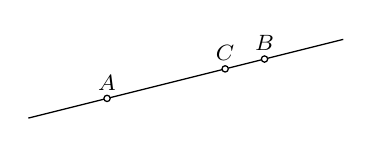
\begin{tikzpicture}
                        % \clip (0,0) rectangle (14.000000,10.000000);
                        {\footnotesize

                        % Drawing line A B
                        \draw [line width=0.016cm] (1.000000,1.250000) -- (1.961194,1.490299);%
                        \draw [line width=0.016cm] (2.038806,1.509701) -- (3.461194,1.865299);%
                        \draw [line width=0.016cm] (3.538806,1.884701) -- (3.961194,1.990299);%
                        \draw [line width=0.016cm] (4.038806,2.009701) -- (5.000000,2.250000);%

                        % Marking point A by circle
                        \draw [line width=0.016cm] (2.000000,1.500000) circle (0.040000);%
                        \draw (2.000000,1.500000) node [anchor=south] { $A$ };%

                        % Marking point C by circle
                        \draw [line width=0.016cm] (3.500000,1.875000) circle (0.040000);%
                        \draw (3.500000,1.875000) node [anchor=south] { $C$ };%

                        % Marking point B by circle
                        \draw [line width=0.016cm] (4.000000,2.000000) circle (0.040000);%
                        \draw (4.000000,2.000000) node [anchor=south] { $B$ };%
                        }
                    \end{tikzpicture}
                \end{figure}
            \end{alertblock}

            \begin{alertblock}{Aksiom}
                Če sta $A$ in $B$ različni točki premice $p$, potem na premici $p$ ležita vsaj še točki $C$ in $D$,
                in sicer $C$ leži med $A$ in $B$, $D$ pa tako, da je $C$ med $A$ in $D$.

                \begin{figure}[H]
                    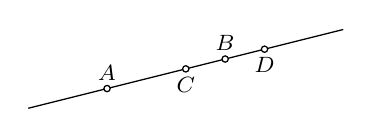
\begin{tikzpicture}
                        % \clip (0,0) rectangle (14.000000,10.000000);
                        {\footnotesize

                        % Drawing line A B
                        \draw [line width=0.016cm] (1.000000,1.250000) -- (1.961194,1.490299);%
                        \draw [line width=0.016cm] (2.038806,1.509701) -- (2.961194,1.740299);%
                        \draw [line width=0.016cm] (3.038806,1.759701) -- (3.461194,1.865299);%
                        \draw [line width=0.016cm] (3.538806,1.884701) -- (3.961194,1.990299);%
                        \draw [line width=0.016cm] (4.038806,2.009701) -- (5.000000,2.250000);%

                        % Marking point A by circle
                        \draw [line width=0.016cm] (2.000000,1.500000) circle (0.040000);%
                        \draw (2.000000,1.500000) node [anchor=south] { $A$ };%

                        % Marking point C by circle
                        \draw [line width=0.016cm] (3.000000,1.750000) circle (0.040000);%
                        \draw (3.000000,1.750000) node [anchor=north] { $C$ };%

                        % Marking point B by circle
                        \draw [line width=0.016cm] (3.500000,1.875000) circle (0.040000);%
                        \draw (3.500000,1.875000) node [anchor=south] { $B$ };%

                        % Marking point D by circle
                        \draw [line width=0.016cm] (4.000000,2.000000) circle (0.040000);%
                        \draw (4.000000,2.000000) node [anchor=north] { $D$ };%
                        }
                    \end{tikzpicture}
                \end{figure}
            \end{alertblock}

            \begin{block}{Izrek}
                Med dvema različnima točkama premice je neskončno mnogo točk.
            \end{block}

        \end{frame}
        

        \begin{frame}
            \begin{alertblock}{Definicija}
                Množica točk premice, ki ležijo med različnima točkama $A$ in $B$, vključno z $A$ in $B$,
                je \textbf{daljica~$AB$}. Točki $A$ in $B$ sta njeni \textbf{krajišči}.

                \begin{figure}[H]
                    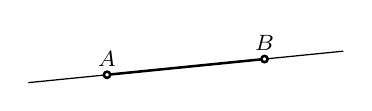
\begin{tikzpicture}
                        % \clip (0,0) rectangle (14.000000,10.000000);
                        {\footnotesize

                        % Drawing line A B
                        \draw [line width=0.016cm] (1.000000,1.400000) -- (1.960199,1.496020);%
                        \draw [line width=0.016cm] (2.039801,1.503980) -- (3.960199,1.696020);%
                        \draw [line width=0.016cm] (4.039801,1.703980) -- (5.000000,1.800000);%

                        % Drawing segment A B
                        \draw [line width=0.032cm] (2.039801,1.503980) -- (3.960199,1.696020);%

                        % Marking point A by circle
                        \draw [line width=0.032cm] (2.000000,1.500000) circle (0.040000);%
                        \draw (2.000000,1.500000) node [anchor=south] { $A$ };%

                        % Marking point B by circle
                        \draw [line width=0.032cm] (4.000000,1.700000) circle (0.040000);%
                        \draw (4.000000,1.700000) node [anchor=south] { $B$ };%
                        }
                    \end{tikzpicture}
                \end{figure}
            \end{alertblock}

            \begin{alertblock}{Definicija}
                Poljubna točka premice razdeli premico na dva \textbf{poltraka}. To točko imenujemo \textbf{izhodišče}, ponavadi jo označimo z $O$.

                \begin{figure}[H]
                    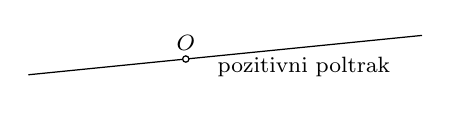
\begin{tikzpicture}
                        % \clip (0,0) rectangle (14.000000,10.000000);
                        {\footnotesize

                        % Drawing line O B
                        \draw [line width=0.016cm] (1.000000,1.300000) -- (2.960199,1.496020);%
                        \draw [line width=0.016cm] (3.039801,1.503980) -- (6.000000,1.800000);%

                        % Marking point O by circle
                        \draw [line width=0.016cm] (3.000000,1.500000) circle (0.040000);%
                        \draw (3.000000,1.500000) node [anchor=south] { $O$ };%

                        % Marking point poz
                        \draw (4.500000,1.400000) node  {pozitivni poltrak };%
                        }
                    \end{tikzpicture}
                \end{figure}
            \end{alertblock}

            \begin{alertblock}{Definicija}
                Premica, na kateri leži daljica oziroma poltrak, je \textbf{nosilka} daljice oziroma poltraka.
            \end{alertblock}
        \end{frame}


        \begin{frame}
            \begin{alertblock}{Definicija}
                \textbf{Enostavni lik} je množica točk v ravnini, ki jo omejuje sklenjena krivulja, ki sama sebe ne seka.
            \end{alertblock}

            \begin{alertblock}{Definicija}
                \begin{columns}
                    \column{0.75\textwidth}

                Množica točk v ravnini je \textbf{konveksna}, če za poljubni točki $A$ in $B$ iz te množice velja, da je daljica $AB$ njena podmnožica.
                $$ \mathcal{M}\text{~konveksna} \Leftrightarrow \forall A, B\in\mathcal{M}\Rightarrow AB\subseteq\mathcal{M} $$
                Množica točk, ki ni konveksna, je \textbf{nekonveksna} oziroma \textbf{konkavna}.
                $$ \mathcal{M}\text{~nekonveksna} \Leftrightarrow \exists A, B\in\mathcal{M}\Rightarrow AB\not\subset\mathcal{M} $$
            
                \column{0.22\textwidth}
                \begin{figure}[H]
                    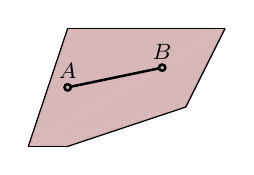
\begin{tikzpicture}
                        % \clip (0,0) rectangle (14.000000,10.000000);
                        {\footnotesize

                        % Changing color 215 183 183
                        \definecolor{r215g183b183}{rgb}{0.843137,0.717647,0.717647}%
                        \color{r215g183b183}% 

                        % Filling triangle C D E
                        \fill (1.500000,1.500000) -- (2.000000,1.500000) -- (3.500000,2.000000);%

                        % Filling triangle C E F
                        \fill (1.500000,1.500000) -- (3.500000,2.000000) -- (4.000000,3.000000);%

                        % Filling triangle C F G
                        \fill (1.500000,1.500000) -- (4.000000,3.000000) -- (2.000000,3.000000);%

                        % Changing color 0 0 0
                        \definecolor{r0g0b0}{rgb}{0.000000,0.000000,0.000000}%
                        \color{r0g0b0}% 

                        % Drawing segment C D
                        \draw [line width=0.016cm] (1.500000,1.500000) -- (2.000000,1.500000);%

                        % Drawing segment D E
                        \draw [line width=0.016cm] (2.000000,1.500000) -- (3.500000,2.000000);%

                        % Drawing segment E F
                        \draw [line width=0.016cm] (3.500000,2.000000) -- (4.000000,3.000000);%

                        % Drawing segment F G
                        \draw [line width=0.016cm] (4.000000,3.000000) -- (2.000000,3.000000);%

                        % Drawing segment G C
                        \draw [line width=0.016cm] (2.000000,3.000000) -- (1.500000,1.500000);%

                        % Marking point A by circle
                        \draw [line width=0.032cm] (2.000000,2.250000) circle (0.040000);%
                        \draw (2.000000,2.250000) node [anchor=south] { $A$ };%

                        % Marking point B by circle
                        \draw [line width=0.032cm] (3.200000,2.500000) circle (0.040000);%
                        \draw (3.200000,2.500000) node [anchor=south] { $B$ };%

                        % Drawing segment A B
                        \draw [line width=0.032cm] (2.039159,2.258158) -- (3.160841,2.491842);%
                        \color{black}
                        }
                    \end{tikzpicture}
                \end{figure}

                \begin{figure}[H]
                    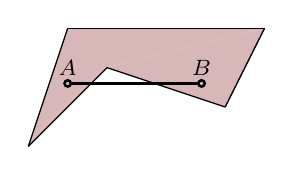
\begin{tikzpicture}
                        % \clip (0,0) rectangle (14.000000,10.000000);
                        {\footnotesize

                        % Changing color 215 183 183
                        \definecolor{r215g183b183}{rgb}{0.843137,0.717647,0.717647}%
                        \color{r215g183b183}% 

                        % Filling triangle C D G
                        \fill (1.500000,1.500000) -- (2.500000,2.500000) -- (2.000000,3.000000);%

                        % Filling triangle D E F
                        \fill (2.500000,2.500000) -- (4.000000,2.000000) -- (4.500000,3.000000);%

                        % Filling triangle D F G
                        \fill (2.500000,2.500000) -- (4.500000,3.000000) -- (2.000000,3.000000);%

                        % Changing color 0 0 0
                        \definecolor{r0g0b0}{rgb}{0.000000,0.000000,0.000000}%
                        \color{r0g0b0}% 

                        % Drawing segment C D
                        \draw [line width=0.016cm] (1.500000,1.500000) -- (2.500000,2.500000);%

                        % Drawing segment D E
                        \draw [line width=0.016cm] (2.500000,2.500000) -- (4.000000,2.000000);%

                        % Drawing segment E F
                        \draw [line width=0.016cm] (4.000000,2.000000) -- (4.500000,3.000000);%

                        % Drawing segment F G
                        \draw [line width=0.016cm] (4.500000,3.000000) -- (2.000000,3.000000);%

                        % Drawing segment G C
                        \draw [line width=0.016cm] (2.000000,3.000000) -- (1.500000,1.500000);%

                        % Marking point A by circle
                        \draw [line width=0.032cm] (2.000000,2.300000) circle (0.040000);%
                        \draw (2.000000,2.300000) node [anchor=south] { $A$ };%

                        % Marking point B by circle
                        \draw [line width=0.032cm] (3.700000,2.300000) circle (0.040000);%
                        \draw (3.700000,2.300000) node [anchor=south] { $B$ };%

                        % Drawing segment A B
                        \draw [line width=0.032cm] (2.040000,2.300000) -- (3.660000,2.300000);%
                        \color{black}
                        }
                    \end{tikzpicture}
                \end{figure}
                \end{columns}

            \end{alertblock}
        \end{frame}


        \begin{frame}
            \begin{alertblock}{Definicija}
                \begin{columns}
                    \column{0.6\textwidth}
                Dva poltraka s skupnim izhodiščem določata dva \textbf{kota}.
                Izhodišče poltrakov imenujemo \textbf{vrh} kota, poltraka pa imenujemo \textbf{kraka} kota.
                
                \column{0.38\textwidth}
                \vskip-2em
                \begin{figure}[H]
                    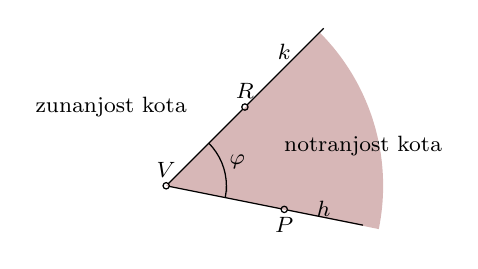
\begin{tikzpicture}
                        % \clip (0,0) rectangle (14.000000,10.000000);
                        {\footnotesize

                        % Changing color 215 183 183
                        \definecolor{r215g183b183}{rgb}{0.843137,0.717647,0.717647}%
                        \color{r215g183b183}% 

                        % Filling circle arc V B 56.31
                        \fill (2.500000,2.500000) -- (5.200000,1.949999) -- (5.204824,1.974235) arc (349:360:2.755449 and 2.755449) --(5.255449,2.500000) arc (0:44:2.755449 and 2.755449) -- (4.455318,4.441451) -- cycle;%

                        % Changing color 0 0 0
                        \definecolor{r0g0b0}{rgb}{0.000000,0.000000,0.000000}%
                        \color{r0g0b0}% 

                        % Drawing line V P
                        % \draw [line width=0.016cm] (1.000000,2.800000) -- (2.460777,2.507845);%
                        \draw [line width=0.016cm] (2.539223,2.492155) -- (3.960777,2.207845);%
                        \draw [line width=0.016cm] (4.039223,2.192155) -- (5.000000,2.000000);%

                        % Drawing line V R
                        % \draw [line width=0.016cm] (1.000000,1.000000) -- (2.471716,2.471716);%
                        \draw [line width=0.016cm] (2.528284,2.528284) -- (3.471716,3.471716);%
                        \draw [line width=0.016cm] (3.528284,3.528284) -- (4.500000,4.500000);%

                        % Marking point V by circle
                        \draw [line width=0.016cm] (2.500000,2.500000) circle (0.040000);%
                        \draw (2.500000,2.500000) node [anchor=south] { $V$ };%

                        % Marking point P by circle
                        \draw [line width=0.016cm] (4.000000,2.200000) circle (0.040000);%
                        \draw (4.000000,2.200000) node [anchor=north] { $P$ };%

                        % Marking point R by circle
                        \draw [line width=0.016cm] (3.500000,3.500000) circle (0.040000);%
                        \draw (3.500000,3.500000) node [anchor=south] { $R$ };%

                        % Marking point h
                        \draw (4.500000,2.000000) node [anchor=south] { $h$ };%

                        % Marking point k
                        \draw (4.000000,4.000000) node [anchor=south] { $k$ };%

                        % Drawing arc V A 56.31
                        \draw [line width=0.016cm] (3.250000,2.350000) -- (3.250800,2.354059) arc (349:360:0.764853 and 0.764853) --(3.264853,2.500000) arc (0:45:0.764853 and 0.764853);%

                        % Marking point \varphi
                        \draw (3.200000,2.800000) node [anchor=west] { $\varphi$ };%

                        % Marking point zun
                        \draw (1.800000,3.500000) node  { zunanjost kota };%

                        % Marking point not
                        \draw (5.000000,3.000000) node  { notranjost kota };%
                        \color{black}
                        }
                    \end{tikzpicture}
                \end{figure}
            \end{columns}
            \end{alertblock}

            \begin{block}{}
                Če poltraka ne ležita na isti premici, je eden od kotov konveksen, drugi pa je nekonveksen.
            \end{block}

            \begin{block}{}
                Kot lahko označimo na več načinov:
                \begin{itemize}
                    \item $\angle(h,k)$, kjer sta $h$ in $k$ poltraka, ki kot določata;
                    \item $\angle PVR$, kjer je $P$ točka na enem poltraku, $V$ vrh kota in $R$ točka na drugem poltraku;
                    \item $\alpha, \beta, \gamma, \dots$ -- z grškimi črkami.
                \end{itemize}
            \end{block}
        \end{frame}


        \begin{frame}
            \begin{alertblock}{Definicija}
                Če poltraka s skupnim izhodiščem ležita na isti premici, vendar na različnih straneh izhodišča,
                določata dva enaka konveksna kota -- \textbf{iztegnjena kota}.

                \begin{figure}[H]
                    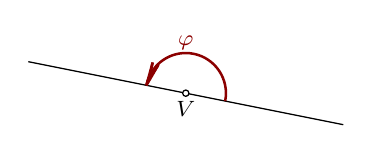
\begin{tikzpicture}
                        % \clip (0,0) rectangle (14.000000,10.000000);
                        {\footnotesize

                        % Drawing line V h
                        \draw [line width=0.016cm] (1.000000,2.000000) -- (2.960777,1.607845);%
                        \draw [line width=0.016cm] (3.039223,1.592155) -- (5.000000,1.200000);%

                        % Marking point V by circle
                        \draw [line width=0.016cm] (3.000000,1.600000) circle (0.040000);%
                        \draw (3.000000,1.600000) node [anchor=north] { $V$ };%

                        % Changing color 139 0 0
                        \definecolor{r139g0b0}{rgb}{0.545098,0.000000,0.000000}%
                        \color{r139g0b0}% 

                        % Drawing arc V h 180.00
                        \draw [line width=0.032cm] (3.500000,1.500000) -- (3.500534,1.502706) arc (349:360:0.509902 and 0.509902) --(3.509902,1.600000) arc (0:168:0.509902 and 0.509902) -- (2.500000,1.700000);%

                        % Marking point \varphi
                        \draw (3.000000,2.050000) node [anchor=south] { $\varphi$ };%

                        % Drawing arrow C A 1.00
                        \draw [line width=0.032cm] (2.651137,1.959148) -- (2.500000,1.700000);%
                        \draw [line width=0.032cm] (2.651137,1.959148) -- (2.538342,1.791430);%
                        \draw [line width=0.032cm] (2.578914,1.989435) -- (2.500000,1.700000);%
                        \draw [line width=0.032cm] (2.578914,1.989435) -- (2.538342,1.791430);%
                        \color{black}
                        }
                    \end{tikzpicture}
                \end{figure}
            \end{alertblock}

            \begin{alertblock}{Definicija}
                Če se poltraka na isti premici prekrivata, določata \textbf{polni kot} ali \textbf{ničelni kot}.

                \begin{figure}[H]
                    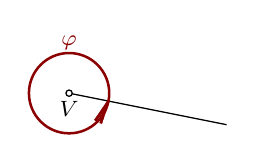
\begin{tikzpicture}
                        % \clip (0,0) rectangle (14.000000,10.000000);
                        {\footnotesize

                        % Drawing line V h
                        % \draw [line width=0.016cm] (1.000000,2.000000) -- (2.960777,1.607845);%
                        \draw [line width=0.016cm] (3.039223,1.592155) -- (5.000000,1.200000);%

                        % Marking point V by circle
                        \draw [line width=0.016cm] (3.000000,1.600000) circle (0.040000);%
                        \draw (3.000000,1.600000) node [anchor=north] { $V$ };%

                        % Changing color 139 0 0
                        \definecolor{r139g0b0}{rgb}{0.545098,0.000000,0.000000}%
                        \color{r139g0b0}% 

                        % Drawing arc V h 360.00
                        \draw [line width=0.032cm] (3.000000,1.600000) circle (0.509902);%

                        % Marking point \varphi
                        \draw (3.000000,2.050000) node [anchor=south] { $\varphi$ };%

                        % Drawing arrow k h 1.00
                        \draw [line width=0.032cm] (3.331960,1.251479) -- (3.500000,1.500000);%
                        \draw [line width=0.032cm] (3.331960,1.251479) -- (3.455661,1.411322);%
                        \draw [line width=0.032cm] (3.402008,1.216456) -- (3.500000,1.500000);%
                        \draw [line width=0.032cm] (3.402008,1.216456) -- (3.455661,1.411322);%
                        \color{black}
                        }
                    \end{tikzpicture} ~~~~~
                    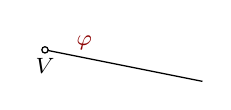
\begin{tikzpicture}
                        % \clip (0,0) rectangle (14.000000,10.000000);
                        {\footnotesize

                        % Drawing line V h
                        % \draw [line width=0.016cm] (1.000000,2.000000) -- (2.960777,1.607845);%
                        \draw [line width=0.016cm] (3.039223,1.592155) -- (5.000000,1.200000);%

                        % Marking point V by circle
                        \draw [line width=0.016cm] (3.000000,1.600000) circle (0.040000);%
                        \draw (3.000000,1.600000) node [anchor=north] { $V$ };%

                        % Changing color 139 0 0
                        \definecolor{r139g0b0}{rgb}{0.545098,0.000000,0.000000}%
                        \color{r139g0b0}% 

                        % Marking point \varphi
                        \draw (3.500000,1.500000) node [anchor=south] { $\varphi$ };%
                        \color{black}
                        }
                    \end{tikzpicture}
                \end{figure}

            \end{alertblock}
        \end{frame}


        \begin{frame}
            \begin{alertblock}{Definicija}
                Kota s skupnim vrhom, ki imata en skupen krak, presek njunih notranjosti pa je prazen, sta \textbf{sosedna kota}.

                \begin{figure}[H]
                    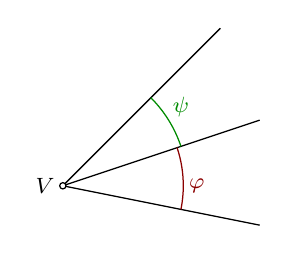
\begin{tikzpicture}
                        % \clip (0,0) rectangle (14.000000,10.000000);
                        {\footnotesize

                        % Drawing line V P
                        \draw [line width=0.016cm] (4.000000,1.000000) -- (1.539223,1.492155);%
                        % \draw [line width=0.016cm] (1.460777,1.507845) -- (1.000000,1.600000);%

                        % Drawing line V Q
                        % \draw [line width=0.016cm] (1.000000,1.333333) -- (1.462053,1.487351);%
                        \draw [line width=0.016cm] (1.537947,1.512649) -- (4.000000,2.333333);%

                        % Drawing line V R
                        % \draw [line width=0.016cm] (1.000000,1.000000) -- (1.471716,1.471716);%
                        \draw [line width=0.016cm] (1.528284,1.528284) -- (3.500000,3.500000);%

                        % Marking point V by circle
                        \draw [line width=0.016cm] (1.500000,1.500000) circle (0.040000);%
                        \draw (1.500000,1.500000) node [anchor=east] { $V$ };%

                        % Changing color 139 0 0
                        \definecolor{r139g0b0}{rgb}{0.545098,0.000000,0.000000}%
                        \color{r139g0b0}% 

                        % Drawing arc V P 29.74
                        \draw [line width=0.016cm] (3.000000,1.200000) -- (3.001601,1.208118) arc (349:360:1.529706 and 1.529706) --(3.029706,1.500000) arc (0:18:1.529706 and 1.529706) -- (2.951206,1.983735);%

                        % Marking point \varphi
                        \draw (3.200000,1.500000) node  { $\varphi$ };%

                        % Changing color 0 139 0
                        \definecolor{r0g139b0}{rgb}{0.000000,0.545098,0.000000}%
                        \color{r0g139b0}% 

                        % Drawing arc V Q 26.57
                        \draw [line width=0.016cm] (3.000000,2.000000) -- (2.994996,2.014768) arc (19:45:1.581139 and 1.581139);%

                        % Marking point \psi
                        \draw (3.000000,2.500000) node  { $\psi$ };%
                        \color{black}
                        }
                    \end{tikzpicture}
                \end{figure}
            % \end{alertblock}

            % \begin{alertblock}{Definicija}
                Sosedna kota, katerih kraka, ki  nista skupna, ležita na isti premici, sta \textbf{sokota}.
                
                \begin{figure}[H]
                    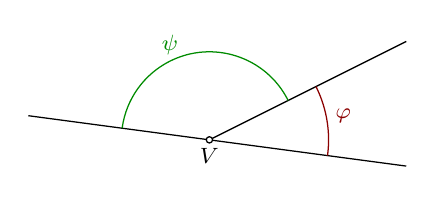
\begin{tikzpicture}
                        % \clip (0,0) rectangle (14.000000,10.000000);
                        {\footnotesize

                        % Drawing line V P
                        \draw [line width=0.016cm] (1.200000,1.806667) -- (3.460351,1.505287);%
                        \draw [line width=0.016cm] (3.539649,1.494713) -- (6.000000,1.166667);%

                        % Drawing line V Q
                        % \draw [line width=0.016cm] (2.700000,1.100000) -- (3.464223,1.482111);%
                        \draw [line width=0.016cm] (3.535777,1.517889) -- (6.000000,2.750000);%

                        % Marking point V by circle
                        \draw [line width=0.016cm] (3.500000,1.500000) circle (0.040000);%
                        \draw (3.500000,1.500000) node [anchor=north] { $V$ };%

                        % Changing color 139 0 0
                        \definecolor{r139g0b0}{rgb}{0.545098,0.000000,0.000000}%
                        \color{r139g0b0}% 

                        % Drawing arc V P 34.16
                        \draw [line width=0.016cm] (5.000000,1.300000) -- (5.001995,1.315578) arc (353:360:1.513275 and 1.513275) --(5.013275,1.500000) arc (0:26:1.513275 and 1.513275) -- (4.853514,2.176757);%

                        % Marking point \varphi
                        \draw (5.200000,1.800000) node  { $\varphi$ };%

                        % Changing color 0 139 0
                        \definecolor{r0g139b0}{rgb}{0.000000,0.545098,0.000000}%
                        \color{r0g139b0}% 

                        % Drawing arc V Q 145.84
                        \draw [line width=0.016cm] (4.500000,2.000000) -- (4.496176,2.007577) arc (27:172:1.118034 and 1.118034) -- (2.391774,1.647764);%

                        % Marking point \psi
                        \draw (3.000000,2.700000) node  { $\psi$ };%
                        \color{black}
                        }
                    \end{tikzpicture}
                \end{figure}
            \end{alertblock}

        \end{frame}


        \begin{frame}
            \begin{alertblock}{Definicija}
                Tri nekolinearne točke $A$, $B$ in $C$ določajo \textbf{trikotnik} $\triangle ABC$.
                Točke $A$, $B$ in $C$ so \textbf{oglišča} trikotnika, daljice $AB$, $BC$ in $AC$ so njegove \textbf{stranice}.

            \begin{figure}
                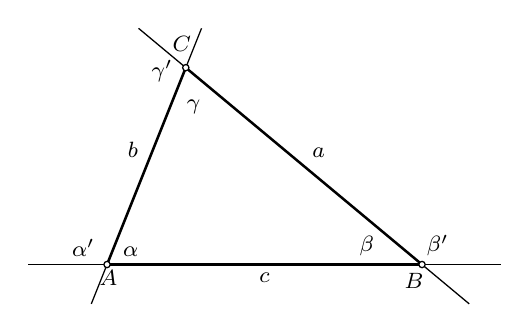
\begin{tikzpicture}
                    % \clip (0,0) rectangle (14.000000,10.000000);
                    {\footnotesize
                    
                    % Marking point A by circle
                    \draw<2-> [line width=0.016cm] (2.000000,1.500000) circle (0.040000);%
                    \draw<2-> (1.800000,1.530000) node [anchor=north west] { $A$ };%
                    
                    % Marking point B by circle
                    \draw<2-> [line width=0.016cm] (6.000000,1.500000) circle (0.040000);%
                    \draw<2-> (5.900000,1.500000) node [anchor=north] { $B$ };%
                    
                    % Marking point C by circle
                    \draw<2-> [line width=0.016cm] (3.000000,4.000000) circle (0.040000);%
                    \draw<2-> (2.950000,4.100000) node [anchor=south] { $C$ };%
                    
                    % Drawing line A B
                    \draw<4-> [line width=0.016cm] (1.000000,1.500000) -- (1.960000,1.500000);%
                    \draw<4-> [line width=0.016cm] (2.040000,1.500000) -- (5.960000,1.500000);%
                    \draw<4-> [line width=0.016cm] (6.040000,1.500000) -- (7.000000,1.500000);%
                    
                    % Drawing line B C
                    \draw<4-> [line width=0.016cm] (6.600000,1.000000) -- (6.030729,1.474393);%
                    \draw<4-> [line width=0.016cm] (5.969271,1.525607) -- (3.030729,3.974393);%
                    \draw<4-> [line width=0.016cm] (2.969271,4.025607) -- (2.400000,4.500000);%
                    
                    % Drawing line A C
                    \draw<4-> [line width=0.016cm] (1.800000,1.000000) -- (1.985144,1.462861);%
                    \draw<4-> [line width=0.016cm] (2.014856,1.537139) -- (2.985144,3.962861);%
                    \draw<4-> [line width=0.016cm] (3.014856,4.037139) -- (3.200000,4.500000);%
                    
                    % Marking point c
                    \draw<2-> (4.000000,1.500000) node [anchor=north] { $c$ };%
                    
                    % Marking point a
                    \draw<2-> (4.500000,2.750000) node [anchor=south west] { $a$ };%
                    
                    % Marking point b
                    \draw<2-> (2.500000,2.750000) node [anchor=south east] { $b$ };%
                    
                    % Marking point \gamma
                    \draw<3-> (3.100000,3.700000) node [anchor=north] { $\gamma$ };%
                    
                    % Marking point \gamma'
                    \draw<4-> (2.700000,4.200000) node [anchor=north] { $\gamma'$ };%
                    
                    % Marking point \beta
                    \draw<3-> (5.300000,1.500000) node [anchor=south] { $\beta$ };%
                    
                    % Marking point \beta'
                    \draw<4-> (6.200000,1.500000) node [anchor=south] { $\beta'$ };%
                    
                    % Marking point \alpha
                    \draw<3-> (2.300000,1.500000) node [anchor=south] { $\alpha$ };%
                    
                    % Marking point \alpha'
                    \draw<4-> (1.700000,1.500000) node [anchor=south] { $\alpha'$ };%
                    
                    % Drawing segment A B
                    \draw<2-> [line width=0.032cm] (2.040000,1.500000) -- (5.960000,1.500000);%
                    
                    % Drawing segment B C
                    \draw<2-> [line width=0.032cm] (5.969271,1.525607) -- (3.030729,3.974393);%
                    
                    % Drawing segment A C
                    \draw<2-> [line width=0.032cm] (2.014856,1.537139) -- (2.985144,3.962861);%
                    }
                \end{tikzpicture}
            \end{figure}

                Koti $\alpha$, $\beta$ in $\gamma$ so \textbf{notranji koti}, 
                njihovi sokoti $\alpha'$, $\beta'$ in $\gamma'$ pa so \textbf{zunanji koti} trikotnika.

            \end{alertblock}

            \begin{block}{}
                Trikotnik je \textbf{pozitivno orientiran}, če si njegova oglišča sledijo v nasprotni smeri vrtenja urnega kazalca; 
                če si sledijo v smeri vrtenja urnega kazalca, pa je \textbf{negativno orientiran}.
            \end{block}
        \end{frame}


        \begin{frame}
            \begin{alertblock}{Definicija}
                Točke $A_1, A_2, A_3, \dots, A_n$ v ravnini, od katerih nobene zaporedne tri niso kolinearne, določajo \textbf{$n$-kotnik}.

                Točke $A_1, A_2, A_3, \dots, A_n$ so \textbf{oglišča} $n$-kotnika;
                daljice, ki povezujejo sosedni oglišči, $A_1A_2, A_2A_3, \dots, A_nA_1$ so \textbf{stranice} $n$-kotnika;
                daljice, ki povezujejo po dve nesosedni oglišči, pa so \textbf{diagonale} $n$-kotnika.
            \end{alertblock}

            \begin{block}{}
                Poljuben $n$-kotnika ima $$\dfrac{n(n-3)}{2}$$ diagonal -- iz vsakega od $n$ oglišč gre $n-3$ diagonal, vsaka pa je šteta dvakrat.
            \end{block}

            \begin{block}{}
                Če za vsako nosilko stranice $n$-kotnika velja, da preostala oglišča ležijo na isti strani te nosilke, je $n$-kotnik \textbf{konveksen}.
            \end{block}
        \end{frame}




        %%%%% naloge

        \begin{frame}

            \only<2->{\begin{exampleblock}{Naloga}
                Izračunajte število diagonal: $17$-kotnika, $31$-kotnika in $28$-kotnika.                
            \end{exampleblock}}

            \only<3->{\begin{exampleblock}{Naloga}
                Ugotovite, ali obstaja $n$-kotnik, ki ima desetino toliko diagonal kot $28$-kotnik.
                Če obstaja, izračunajte, koliko stranic ima.
            \end{exampleblock}}   
            
            \only<4->{\begin{exampleblock}{Naloga}
                Kateri $n$-kotnik ima štirikrat toliko diagonal kot stranic?
            \end{exampleblock}}
        
            \only<5->{\begin{exampleblock}{Naloga}
                Izračunajte, kateri $n$-kotnik ima: $104$ diagonale, $230$ diagonal, $2n-5$ diagonal.
            \end{exampleblock}}

            \only<6->{\begin{exampleblock}{Naloga}
                Pokažite, da ne obstaja $n$-kotnik, ki ima $13$ diagonal.  
            \end{exampleblock}}
            
        \end{frame}


        \begin{frame}

            \only<2->{\begin{exampleblock}{Naloga}
                Za vsako od spodnjih izjav ugotovite, ali je pravilna ali nepravilna.
                \begin{itemize}
                    \item Tri različne točke, so vedno nekolinearne.
                    \item Petkotnik ima enako število diagonal in stranic.
                    \item Štiri različne premice se sekajo v največ $4$ različnih točkah.
                    \item Skozi štiri kolinearne točke gredo tri različne premice.
                    \item Vzporedni premici imata lahko neskončno mnogo skupnih točk.
                \end{itemize}
            \end{exampleblock}}

            \only<3->{\begin{exampleblock}{Naloga}
                Pokažite, da je število diagonal $25$-kotnika večkratnik števila njegovih stranic.
            \end{exampleblock}}

            \only<4->{\begin{exampleblock}{Naloga}
                Vsota števila stranic in diagonal $n$-kotnika je $105$? Kateri $n$-kotnik je to?
            \end{exampleblock}}

        \end{frame}


        \begin{frame}

            \only<2->{\begin{exampleblock}{Naloga}
                Izračunajte, kateri $n$-kotnik ima toliko diagonal kot stranic.
            \end{exampleblock}}

            \only<3->{\begin{exampleblock}{Naloga}
                Člani filatelističnega društva so se domenili, da si bodo za praznike spet pošiljali voščilnice po klasični pošti.
                Ko so se dobili po novem letu, so prinesli vse voščilnice in jih našteli $132$.
                Izračunajte, koliko članov društva, si je medseboj poslalo voščilnice.                
            \end{exampleblock}}


        \end{frame}





%%%%%%%%%%%%%%%%%%%%%%%%%%%%%%%%%%%%%
    \subsection{Skladnost in merjenje}

        \begin{frame}
            \frametitle{Skladnost}

            \begin{alertblock}{Definicija}
                Dva lika $L$ in $L'$ sta \textbf{skladna}, če lahko lik $L$ prenesemo na lik $L'$ tako,
                da se popolnoma prekrijeta.

                Znak za skladnost je $\cong$.
            \end{alertblock}

            \begin{block}{}
                \textbf{Skladnost} je v množici ravninskih likov \textit{ekvivalenčna relacija}, saj je:
                \begin{itemize}
                    \item \textit{refleksivna}: $L\cong L$ -- vsaka množica je skladna sama s seboj;
                    \item \textit{simetrična}: $L\cong L' \Rightarrow L'\cong L$ -- če je prva množica skladna z drugo, je tudi druga skladna s prvo;
                    \item \textit{tranzitivna}: $L\cong L' \land L'\cong L'' \rightarrow L\cong L''$ -- če je prva množica skladna z drugo in druga skladna s tretjo, 
                            je tudi prva množica skladna s tretjo množico.
                \end{itemize}
            \end{block}
        \end{frame}


        \begin{frame}
            \begin{alertblock}{Definicija}
                Kot, ki je skladen s svojim sokotom, je \textbf{pravi kot}.

                \begin{figure}[H]
                    \begin{tikzpicture}
                    % \clip (0,0) rectangle (14.000000,10.000000);
                    {\footnotesize

                    % Drawing line V A
                    \draw [line width=0.016cm] (1.000000,1.500000) -- (2.960000,1.500000);%
                    \draw [line width=0.016cm] (3.040000,1.500000) -- (5.000000,1.500000);%

                    % Drawing line V B
                    % \draw [line width=0.016cm] (3.000000,1.000000) -- (3.000000,1.460000);%
                    \draw [line width=0.016cm] (3.000000,1.540000) -- (3.000000,3.500000);%

                    % Marking point V by circle
                    \draw [line width=0.016cm] (3.000000,1.500000) circle (0.040000);%

                    % Changing color 139 0 0
                    \definecolor{r139g0b0}{rgb}{0.545098,0.000000,0.000000}%
                    \color{r139g0b0}% 

                    % Drawing arc V A 90.00
                    \draw [line width=0.032cm] (3.800000,1.500000) arc (360:360:0.800000 and 0.800000) --(3.800000,1.500000) arc (0:90:0.800000 and 0.800000);%

                    % Changing color 0 139 0
                    \definecolor{r0g139b0}{rgb}{0.000000,0.545098,0.000000}%
                    \color{r0g139b0}% 

                    % Drawing arc V B 90.00
                    \draw [line width=0.032cm] (3.000000,2.200000) arc (90:180:0.700000 and 0.700000);%
                    \color{black}
                    }
                    \end{tikzpicture}

                \end{figure}
                
            \end{alertblock}

            \begin{block}{}
                Če si kraka sledita v nasprotni smeri vrtenja urnega kazalca, je \textbf{orientacija kota pozitivna}, 
                če pa si sledita v smeri vrtenja urnega kazalca, pa je \textbf{orientacija kota negativna}.

                \begin{figure}[H]
                    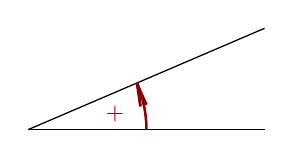
\begin{tikzpicture}
                    % \clip (0,0) rectangle (14.000000,10.000000);
                    {\footnotesize

                    % Drawing segment A b
                    \draw [line width=0.016cm] (1.500000,1.500000) -- (4.500000,1.500000);%

                    % Drawing segment A C
                    \draw [line width=0.016cm] (1.500000,1.500000) -- (4.500000,2.785714);%

                    % Changing color 139 0 0
                    \definecolor{r139g0b0}{rgb}{0.545098,0.000000,0.000000}%
                    \color{r139g0b0}% 

                    % Drawing arc A B 23.20
                    \draw [line width=0.032cm] (3.000000,1.500000) arc (360:360:1.500000 and 1.500000) --(3.000000,1.500000) arc (0:23:1.500000 and 1.500000) -- (2.878718,2.090879);%

                    % Drawing arrow Bb U 1.00
                    \draw [line width=0.032cm] (2.923918,1.794304) -- (2.878718,2.090879);%
                    \draw [line width=0.032cm] (2.923918,1.794304) -- (2.906321,1.995655);%
                    \draw [line width=0.032cm] (2.999137,1.816108) -- (2.878718,2.090879);%
                    \draw [line width=0.032cm] (2.999137,1.816108) -- (2.906321,1.995655);%

                    % Marking point +
                    \draw (2.600000,1.700000) node  { $+$ };%
                    \color{black}
                    }
                    \end{tikzpicture} ~~~~~
                    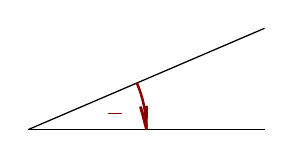
\begin{tikzpicture}
                    % \clip (0,0) rectangle (14.000000,10.000000);
                    {\footnotesize

                    % Drawing segment A b
                    \draw [line width=0.016cm] (1.500000,1.500000) -- (4.500000,1.500000);%

                    % Drawing segment A C
                    \draw [line width=0.016cm] (1.500000,1.500000) -- (4.500000,2.785714);%

                    % Changing color 139 0 0
                    \definecolor{r139g0b0}{rgb}{0.545098,0.000000,0.000000}%
                    \color{r139g0b0}% 

                    % Drawing arc A B 23.20
                    \draw [line width=0.032cm] (3.000000,1.500000) arc (360:360:1.500000 and 1.500000) --(3.000000,1.500000) arc (0:23:1.500000 and 1.500000) -- (2.878718,2.090879);%

                    % Drawing arrow Bb B 1.00
                    \draw [line width=0.032cm] (3.001963,1.799994) -- (3.000000,1.500000);%
                    \draw [line width=0.032cm] (3.001963,1.799994) -- (2.987703,1.598379);%
                    \draw [line width=0.032cm] (2.924252,1.790280) -- (3.000000,1.500000);%
                    \draw [line width=0.032cm] (2.924252,1.790280) -- (2.987703,1.598379);%

                    % Marking point -
                    \draw (2.600000,1.700000) node  { $-$ };%
                    \color{black}
                    }
                    \end{tikzpicture}
                \end{figure}
            \end{block}
        \end{frame}

        \begin{frame}
            \frametitle{Merjenje}

            \vskip-1.5em
            \begin{block}{}
                Daljici $AB$ in $CD$, ki nista skladni, lahko premaknemo na poljubni premici tako,
                da levi krajišči sovpadata in da eno od desnih krajišč, npr. $D$ leži med $A$ in $B$.
                V tem primeru je daljica $AB$ \textbf{daljša} od daljice $CD$ oziroma je daljica $CD$ \textbf{krajša} od daljice $AB$.
            \end{block}

            \begin{alertblock}{Arhimedov aksiom}
                Obstaja tako naravno število $n$, pri katerem je vsota $n$ krajših daljic $CD$ daljša od daljice $AB$,
                vsota $n-1$ krajših daljic $CD$ pa je kvečjemu skladna z daljico $AB$.
                % $$n\cdot |CD|>|AB| \quad \quad (n-1)\cdot |CD|\leq |AB|$$

                \begin{figure}[H]
                    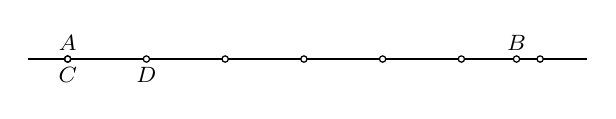
\begin{tikzpicture}
                    % \clip (0,0) rectangle (14.000000,10.000000);
                    {\footnotesize

                    % Drawing line A B
                    \draw [line width=0.016cm] (1.000000,1.500000) -- (1.460000,1.500000);%
                    \draw [line width=0.016cm] (1.540000,1.500000) -- (2.460000,1.500000);%
                    \draw [line width=0.016cm] (2.540000,1.500000) -- (3.460000,1.500000);%
                    \draw [line width=0.016cm] (3.540000,1.500000) -- (4.460000,1.500000);%
                    \draw [line width=0.016cm] (4.540000,1.500000) -- (5.460000,1.500000);%
                    \draw [line width=0.016cm] (5.540000,1.500000) -- (6.460000,1.500000);%
                    \draw [line width=0.016cm] (6.540000,1.500000) -- (7.160000,1.500000);%
                    \draw [line width=0.016cm] (7.240000,1.500000) -- (7.460000,1.500000);%
                    \draw [line width=0.016cm] (7.540000,1.500000) -- (8.100000,1.500000);%

                    % Marking point A by circle
                    \draw [line width=0.016cm] (1.500000,1.500000) circle (0.040000);%
                    \draw (1.500000,1.500000) node [anchor=south] { $A$ };%

                    % Marking point B by circle
                    \draw [line width=0.016cm] (7.200000,1.500000) circle (0.040000);%
                    \draw (7.200000,1.500000) node [anchor=south] { $B$ };%

                    % Marking point C by circle
                    \draw [line width=0.016cm] (1.500000,1.500000) circle (0.040000);%
                    \draw (1.500000,1.500000) node [anchor=north] { $C$ };%

                    % Marking point D by circle
                    \draw [line width=0.016cm] (2.500000,1.500000) circle (0.040000);%
                    \draw (2.500000,1.500000) node [anchor=north] { $D$ };%

                    % Marking point E by circle
                    \draw [line width=0.016cm] (3.500000,1.500000) circle (0.040000);%

                    % Marking point F by circle
                    \draw [line width=0.016cm] (4.500000,1.500000) circle (0.040000);%

                    % Marking point G by circle
                    \draw [line width=0.016cm] (5.500000,1.500000) circle (0.040000);%

                    % Marking point H by circle
                    \draw [line width=0.016cm] (6.500000,1.500000) circle (0.040000);%

                    % Marking point I by circle
                    \draw [line width=0.016cm] (7.500000,1.500000) circle (0.040000);%
                    }
                    \end{tikzpicture}
                \end{figure}
            \end{alertblock}

            % \begin{block}{}
            %     Daljico $CD$, s katero smo izmerili daljico $AB$, imenujemo \textbf{enotska daljica}.
            %     Tako smo daljici $AB$ priredili natančno določeno število -- \textbf{dolžino} daljice $AB$ oziroma \textbf{razdaljo} točk $A$ in $B$.
            %     $$ |AB|=d(A,B)$$
            % \end{block}
            \begin{block}{}
                Daljico $CD$ imenujemo \textbf{enotska daljica}.
                Daljici $AB$ smo priredili natančno določeno število -- \textbf{dolžino} daljice $AB$ oziroma \textbf{razdaljo} točk $A$ in $B$.
                \vskip-1em
                $$ |AB|=d(A,B)$$
            \end{block}

        \end{frame}


        \begin{frame}
            \begin{alertblock}{Aksiom}
                Če je $AB$ poljubna daljica, $A'$ pa točka na poljubnem poltraku, obstaja na tem poltraku natančno določena točka $B'$,
                da je daljica $A'B'$ skladna z daljico $AB$.
                \vskip-1em
                $$A'B'\cong AB$$
            \end{alertblock}

            \begin{block}{Izrek}
                Skladni daljici imata enako dolžino.
                % $$|A'B'|=|AB|$$
            \end{block}

            \begin{alertblock}{Aksiom}
                Naj daljici $AB$ in $BC$ ležita na isti premici in naj imata skupno le točko $B$.
                Daljici $A'B'$ in $B'C'$ naj ležita na tej ali neki drugi premici in naj imata skupno točko $B'$.
                Če velja $AB\cong A'B'$ in $BC\cong B'C'$, potem velja tudi $AC\cong A'C'$.
            \end{alertblock}

            \begin{block}{Izrek}
                Dolžina vsote daljic je enaka vsoti dolžin posameznih daljic.
            \end{block}
        \end{frame}


        \begin{frame}
            \frametitle{Enote}

            \vskip-1em
            \begin{block}{}
                Osnovna enota za merjenje dolžine je \textbf{meter}.

                Iz nje izpeljane enote pa so \textit{decimeter}, \textit{centimeter}, \textit{milimeter}, \textit{kilometer} itd.
                $$ 1~m=10~dm=100~cm=1000~mm$$  $$1~km=1000~m$$ 
            \end{block}

            \begin{block}{}
                Enota za merjenje kotov je \textbf{kotna stopinja} -- velikost $\dfrac{1}{360}$ polnega kota.
                
                Izpeljani enoti sta \textit{(kotna) minuta} in \textit{(kotna) sekunda}.
                $$1^\circ=60'=3600''$$ 
            \end{block}

            \begin{block}{}
                Velikost kota nič je $0^\circ$, pravega kota je $90^\circ$, iztegnjenega kota je $180^\circ$, polnega kota pa je $360^\circ$.
            \end{block}
        \end{frame}


        \begin{frame}
            \begin{alertblock}{Definicija}
                Kota $\varphi$ in $\psi$, katerih vsota meri $180^\circ$, sta \textbf{suplementarna kota}.

                \begin{figure}[H]
                    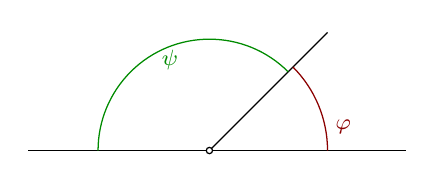
\begin{tikzpicture}
                    % \clip (0,0) rectangle (14.000000,10.000000);
                    {\footnotesize

                    % Drawing line V P
                    \draw [line width=0.016cm] (1.200000,1.500000) -- (3.460000,1.500000);%
                    \draw [line width=0.016cm] (3.540000,1.500000) -- (6.000000,1.500000);%

                    % Drawing line V Q
                    % \draw [line width=0.016cm] (3.100000,1.100000) -- (3.471716,1.471716);%
                    \draw [line width=0.016cm] (3.528284,1.528284) -- (5.000000,3.000000);%

                    % Marking point V by circle
                    \draw [line width=0.016cm] (3.500000,1.500000) circle (0.040000);%

                    % Changing color 139 0 0
                    \definecolor{r139g0b0}{rgb}{0.545098,0.000000,0.000000}%
                    \color{r139g0b0}% 

                    % Drawing arc V P 45.00
                    \draw [line width=0.016cm] (5.000000,1.500000) arc (360:360:1.500000 and 1.500000) --(5.000000,1.500000) arc (0:45:1.500000 and 1.500000);%

                    % Marking point \varphi
                    \draw (5.200000,1.80000) node  { $\varphi$ };%

                    % Changing color 0 139 0
                    \definecolor{r0g139b0}{rgb}{0.000000,0.545098,0.000000}%
                    \color{r0g139b0}% 

                    % Drawing arc V Q 135.00
                    \draw [line width=0.016cm] (4.500000,2.500000) arc (45:180:1.414214 and 1.414214);%

                    % Marking point \psi
                    \draw (3.000000,2.650000) node  { $\psi$ };%
                    \color{black}
                    }
                    \end{tikzpicture}
                \end{figure}
            \end{alertblock}

                        
            \begin{alertblock}{Definicija}
                Kota $\varphi$ in $\psi$, katerih vsota meri $90^\circ$, sta \textbf{komplementarna kota}.

                \begin{figure}[H]
                    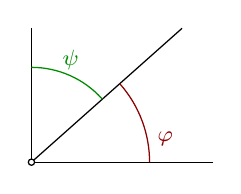
\begin{tikzpicture}
                    % \clip (0,0) rectangle (14.000000,10.000000);
                    {\footnotesize

                    % Drawing line V P
                    % \draw [line width=0.016cm] (2.800000,1.500000) -- (3.460000,1.500000);%
                    \draw [line width=0.016cm] (3.540000,1.500000) -- (5.800000,1.500000);%

                    % Drawing line V Q
                    % \draw [line width=0.016cm] (3.050000,1.100000) -- (3.470104,1.473425);%
                    \draw [line width=0.016cm] (3.529896,1.526575) -- (5.412500,3.200000);%

                    % Drawing line V R
                    % \draw [line width=0.016cm] (3.500000,1.100000) -- (3.500000,1.460000);%
                    \draw [line width=0.016cm] (3.500000,1.540000) -- (3.500000,3.200000);%

                    % Marking point V by circle
                    \draw [line width=0.016cm] (3.500000,1.500000) circle (0.040000);%

                    % Changing color 139 0 0
                    \definecolor{r139g0b0}{rgb}{0.545098,0.000000,0.000000}%
                    \color{r139g0b0}% 

                    % Drawing arc V P 41.63
                    \draw [line width=0.016cm] (5.000000,1.500000) arc (360:360:1.500000 and 1.500000) --(5.000000,1.500000) arc (0:41:1.500000 and 1.500000) -- (4.621114,2.496546);%

                    % Marking point \varphi
                    \draw (5.200000,1.800000) node  { $\varphi$ };%

                    % Changing color 0 139 0
                    \definecolor{r0g139b0}{rgb}{0.000000,0.545098,0.000000}%
                    \color{r0g139b0}% 

                    % Drawing arc V Q 48.37
                    \draw [line width=0.016cm] (4.400000,2.300000) -- (4.394865,2.305740) arc (42:90:1.204159 and 1.204159);%

                    % Marking point \psi
                    \draw (4.000000,2.800000) node  { $\psi$ };%
                    \color{black}
                    }
                    \end{tikzpicture}
                \end{figure}
            \end{alertblock}

            \begin{block}{}
                Sokota sta vedno suplementarna kota.
            \end{block}
        \end{frame}


        \begin{frame}
            \frametitle{Skladnost trikotnikov}

            \vskip-1em
            \begin{alertblock}{Definicija}
                Dva trikotnika sta \textbf{skladna}, če imata paroma skladne vse stranice in tem stranicam nasprotne kote.
            \end{alertblock}

            \begin{alertblock}{Aksiom}
                Dva trikotnika sta skladna, če se ujemata v dveh stranicah in v vmesnem kotu.
            \end{alertblock}

            \begin{block}{Izrek}
                Trikotnika $\triangle ABC$ in $\triangle A'B'C'$ sta skladna, če se ujemata:
                \begin{enumerate}
                    \item v vseh treh stranicah;
                    \item v eni stranici in obeh priležnih kotih;
                    \item v dveh stranicah in kotu, ki leži nasproti daljši od obeh stranic.
                \end{enumerate}
            \end{block}
        \end{frame}



%%%% naloge



        \begin{frame}

            \only<2->{\begin{exampleblock}{Naloga}
                Izračunajte dolžino daljice, če ena polovica meri $2x-7$ enot, druga polovica pa $x+8$ enot.
            \end{exampleblock}}

            \only<3->{\begin{exampleblock}{Naloga}
                Izračunaj dolžino $x$ daljice $AB$, če je točka $S$ njeno razpolovišče, točka $R$ pa razpolovišče daljice $SB$ in je $\lvert SR \rvert = \dfrac{x}{3}-1$.
            \end{exampleblock}}

            \only<4->{\begin{exampleblock}{Naloga}
                Izračunajte velikosti kotov $\alpha$ in $\beta$, če je $\alpha=\beta$.
                Podatke razberite s skice.

                \begin{figure}
                    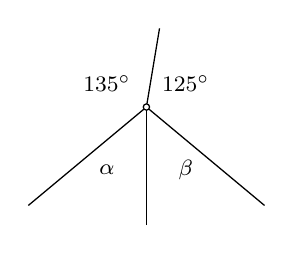
\begin{tikzpicture}
                        % \clip (0,0) rectangle (14.000000,10.000000);
                        {\footnotesize

                        % Marking point A by circle
                        \draw [line width=0.016cm] (3.000000,3.000000) circle (0.040000);%

                        % Drawing segment A B
                        \draw [line width=0.016cm] (3.000000,1.500000) -- (3.000000,2.960000);%

                        % Drawing segment A C
                        \draw [line width=0.016cm] (3.030729,2.974393) -- (4.500000,1.750000);%

                        % Drawing segment A D
                        \draw [line width=0.016cm] (2.969271,2.974393) -- (1.500000,1.750000);%

                        % Drawing segment A E
                        \draw [line width=0.016cm] (3.006576,3.039456) -- (3.166667,4.000000);%

                        % Marking point \beta
                        \draw (3.500000,2.200000) node  { $\beta$ };%

                        % Marking point \alpha
                        \draw (2.500000,2.200000) node  { $\alpha$ };%

                        % Marking point {125^\circ}
                        \draw (3.500000,3.300000) node  { ${125^\circ}$ };%

                        % Marking point {135^\circ}
                        \draw (2.500000,3.300000) node  { ${135^\circ}$ };%
                        }
                    \end{tikzpicture}

                \end{figure}
            \end{exampleblock}}


        \end{frame}


        \begin{frame}
            % \vskip-0.5em
            % \begin{columns}
            % \column{0.33\textwidth}   
            \only<2->{\begin{exampleblock}{Naloga}
                Iz podatkov na skici izračunajte neznano velikost kota $x$.

                \begin{figure}
                    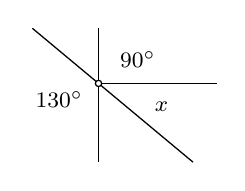
\begin{tikzpicture}
                        % \clip (0,0) rectangle (14.000000,10.000000);
                        {\footnotesize

                        % Marking point A by circle
                        \draw [line width=0.016cm] (3.000000,3.000000) circle (0.040000);%

                        % Drawing line A B
                        \draw [line width=0.016cm] (3.000000,2.000000) -- (3.000000,2.960000);%
                        \draw [line width=0.016cm] (3.000000,3.040000) -- (3.000000,3.700000);%

                        % Drawing line A C
                        \draw [line width=0.016cm] (4.200000,2.000000) -- (3.030729,2.974393);%
                        \draw [line width=0.016cm] (2.969271,3.025607) -- (2.160000,3.700000);%

                        % Drawing segment A E
                        \draw [line width=0.016cm] (3.040000,3.000000) -- (4.500000,3.000000);%

                        % Marking point x
                        \draw (3.800000,2.700000) node  { $x$ };%

                        % Marking point {90^\circ}
                        \draw (3.500000,3.300000) node  { ${90^\circ}$ };%

                        % Marking point {130^\circ}
                        \draw (2.500000,2.800000) node  { ${130^\circ}$ };%
                        }
                    \end{tikzpicture}

                \end{figure}
            \end{exampleblock}}

            % \column{0.63\textwidth}   
            \only<3->{\begin{exampleblock}{Naloga}
                Izračunajte velikosti kotov $\angle AVM$ in $\angle FVE$, če poltrak $VM$ obakrat razpolavlja kot.

                \begin{figure}
                    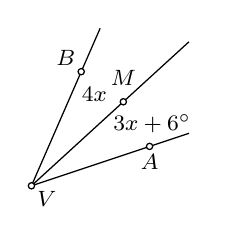
\begin{tikzpicture}
                        % \clip (0,0) rectangle (14.000000,10.000000);
                        {\footnotesize

                        % Marking point V by circle
                        \draw [line width=0.016cm] (1.500000,1.500000) circle (0.040000);%
                        \draw (1.470000,1.530000) node [anchor=north west] { $V$ };%

                        % Marking point A by circle
                        \draw [line width=0.016cm] (3.000000,2.000000) circle (0.040000);%
                        \draw (3.000000,2.000000) node [anchor=north] { $A$ };%

                        % Drawing line V A
                        % \draw [line width=0.016cm] (1.200000,1.400000) -- (1.462053,1.487351);%
                        \draw [line width=0.016cm] (1.537947,1.512649) -- (2.962053,1.987351);%
                        \draw [line width=0.016cm] (3.037947,2.012649) -- (3.500000,2.166667);%

                        % Marking point M by circle
                        \draw [line width=0.016cm] (2.666950,2.566878) circle (0.040000);%
                        \draw (2.666950,2.666878) node [anchor=south] { $M$ };%

                        % Marking point B by circle
                        \draw [line width=0.016cm] (2.132124,2.949283) circle (0.040000);%
                        \draw (2.162124,2.919283) node [anchor=south east] { $B$ };%

                        % Drawing line V B
                        % \draw [line width=0.016cm] (1.369151,1.200000) -- (1.484008,1.463336);%
                        \draw [line width=0.016cm] (1.515992,1.536664) -- (2.116132,2.912618);%
                        \draw [line width=0.016cm] (2.148115,2.985947) -- (2.372326,3.500000);%

                        % Drawing line V M
                        % \draw [line width=0.016cm] (1.200000,1.225727) -- (1.470478,1.473010);%
                        \draw [line width=0.016cm] (1.529522,1.526990) -- (2.637428,2.539888);%
                        \draw [line width=0.016cm] (2.696472,2.593868) -- (3.500000,3.328489);%

                        % Marking point {3x+6^\circ}
                        \draw (3.033475,2.283439) node  { ${3x+6^\circ}$ };%

                        % Marking point {4x}
                        \draw (2.299537,2.658080) node  { ${4x}$ };%
                        }
                    \end{tikzpicture} ~
                    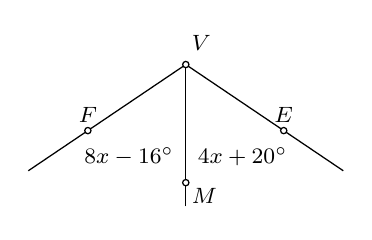
\begin{tikzpicture}
                        % \clip (0,0) rectangle (14.000000,10.000000);
                        {\footnotesize

                        % Marking point V by circle
                        \draw [line width=0.016cm] (4.000000,4.000000) circle (0.040000);%
                        \draw (3.970000,4.070000) node [anchor=south west] { $V$ };%

                        % Marking point M by circle
                        \draw [line width=0.016cm] (4.000000,2.500000) circle (0.040000);%
                        \draw (3.970000,2.530000) node [anchor=north west] { $M$ };%

                        % Drawing line V M
                        \draw [line width=0.016cm] (4.000000,2.200000) -- (4.000000,2.460000);%
                        \draw [line width=0.016cm] (4.000000,2.540000) -- (4.000000,3.960000);%
                        % \draw [line width=0.016cm] (4.000000,4.040000) -- (4.000000,4.200000);%

                        % Marking point F by circle
                        \draw [line width=0.016cm] (2.756444,3.161211) circle (0.040000);%
                        \draw (2.756444,3.161211) node [anchor=south] { $F$ };%

                        % Marking point E by circle
                        \draw [line width=0.016cm] (5.243556,3.161211) circle (0.040000);%
                        \draw (5.243556,3.161211) node [anchor=south] { $E$ };%

                        % Drawing line V E
                        % \draw [line width=0.016cm] (3.703488,4.200000) -- (3.966838,4.022368);%
                        \draw [line width=0.016cm] (4.033162,3.977632) -- (5.210395,3.183578);%
                        \draw [line width=0.016cm] (5.276718,3.138843) -- (6.000000,2.650983);%

                        % Drawing line V F
                        % \draw [line width=0.016cm] (4.296512,4.200000) -- (4.033162,4.022368);%
                        \draw [line width=0.016cm] (3.966838,3.977632) -- (2.789605,3.183578);%
                        \draw [line width=0.016cm] (2.723282,3.138843) -- (2.000000,2.650983);%

                        % Marking point {8x-16^\circ}
                        \draw (3.278222,2.830605) node  { ${8x-16^\circ}$ };%

                        % Marking point {4x+20^\circ}
                        \draw (4.721778,2.830605) node  { ${4x+20^\circ}$ };%
                        }
                    \end{tikzpicture}


                \end{figure}
            \end{exampleblock}}
            % \end{columns}
        \end{frame}


        \begin{frame}

            \only<2->{\begin{exampleblock}{Naloga}
                Izračunajte velikost kota $\angle PVQ$, če je $\angle PVR=94^\circ$.

                \begin{figure}
                    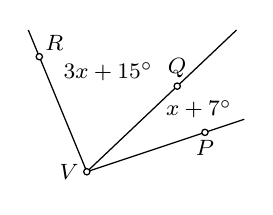
\begin{tikzpicture}
                        % \clip (0,0) rectangle (14.000000,10.000000);
                        {\footnotesize

                        % Marking point V by circle
                        \draw [line width=0.016cm] (3.500000,1.500000) circle (0.040000);%
                        \draw (3.500000,1.500000) node [anchor=east] { $V$ };%

                        % Marking point P by circle
                        \draw [line width=0.016cm] (5.000000,2.000000) circle (0.040000);%
                        \draw (5.000000,2.000000) node [anchor=north] { $P$ };%

                        % Drawing line V P
                        % \draw [line width=0.016cm] (2.600000,1.200000) -- (3.462053,1.487351);%
                        \draw [line width=0.016cm] (3.537947,1.512649) -- (4.962053,1.987351);%
                        \draw [line width=0.016cm] (5.037947,2.012649) -- (5.500000,2.166667);%

                        % Marking point Q by circle
                        \draw [line width=0.016cm] (4.648153,2.587081) circle (0.040000);%
                        \draw (4.648153,2.587081) node [anchor=south] { $Q$ };%

                        % Marking point R by circle
                        \draw [line width=0.016cm] (2.896583,2.961468) circle (0.040000);%
                        \draw (2.866583,2.931468) node [anchor=south west] { $R$ };%

                        % Drawing line V R
                        % \draw [line width=0.016cm] (3.623865,1.200000) -- (3.515265,1.463027);%
                        \draw [line width=0.016cm] (3.484735,1.536973) -- (2.911849,2.924495);%
                        \draw [line width=0.016cm] (2.881318,2.998440) -- (2.756809,3.300000);%

                        % Drawing line V Q
                        % \draw [line width=0.016cm] (3.183146,1.200000) -- (3.470954,1.472499);%
                        \draw [line width=0.016cm] (3.529046,1.527501) -- (4.619106,2.559580);%
                        \draw [line width=0.016cm] (4.677199,2.614582) -- (5.401122,3.300000);%

                        % Marking point {x+7^\circ}
                        \draw (4.924076,2.293541) node  { ${x+7^\circ}$ };%

                        % Marking point {3x+15^\circ}
                        \draw (3.772368,2.774275) node  { ${3x+15^\circ}$ };%
                        }
                    \end{tikzpicture}

                \end{figure}
            \end{exampleblock}}


            \only<3->{\begin{exampleblock}{Naloga}
                Izračunajte velikost kota $\angle SVR$, če je $\angle QVS=50^\circ$.

                \begin{figure}
                    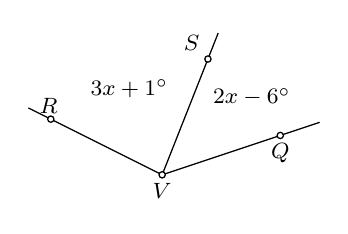
\begin{tikzpicture}
                        % \clip (0,0) rectangle (14.000000,10.000000);
                        {\footnotesize

                        % Marking point V by circle
                        \draw [line width=0.016cm] (3.500000,1.500000) circle (0.040000);%
                        \draw (3.500000,1.500000) node [anchor=north] { $V$ };%

                        % Marking point P by circle
                        \draw [line width=0.016cm] (5.000000,2.000000) circle (0.040000);%
                        \draw (5.000000,2.000000) node [anchor=north] { $Q$ };%

                        % Drawing line V P
                        % \draw [line width=0.016cm] (2.600000,1.200000) -- (3.462053,1.487351);%
                        \draw [line width=0.016cm] (3.537947,1.512649) -- (4.962053,1.987351);%
                        \draw [line width=0.016cm] (5.037947,2.012649) -- (5.500000,2.166667);%

                        % Marking point S by circle
                        \draw [line width=0.016cm] (4.081159,2.970460) circle (0.040000);%
                        \draw (4.081159,2.970460) node [anchor=south east] { $S$ };%

                        % Marking point R by circle
                        \draw [line width=0.016cm] (2.085787,2.207107) circle (0.040000);%
                        \draw (2.055787,2.177107) node [anchor=south] { $R$ };%

                        % Drawing line V R
                        % \draw [line width=0.016cm] (4.100000,1.200000) -- (3.535777,1.482111);%
                        \draw [line width=0.016cm] (3.464223,1.517889) -- (2.121564,2.189218);%
                        \draw [line width=0.016cm] (2.050009,2.224995) -- (1.800000,2.350000);%

                        % Drawing line V S
                        % \draw [line width=0.016cm] (3.381433,1.200000) -- (3.485298,1.462800);%
                        \draw [line width=0.016cm] (3.514702,1.537200) -- (4.066457,2.933260);%
                        \draw [line width=0.016cm] (4.095862,3.007660) -- (4.211401,3.300000);%

                        % Marking point {2x-6^\circ}
                        \draw (4.640580,2.485230) node  { ${2x-6^\circ}$ };%

                        % Marking point {3x+1^\circ}
                        \draw (3.083473,2.588784) node  { ${3x+1^\circ}$ };%
                        }
                    \end{tikzpicture}

                \end{figure}
            \end{exampleblock}}

        \end{frame}

                
        \begin{frame}

            \only<2->{\begin{exampleblock}{Naloga}
                Kot $\varphi=76^\circ 36'53''$ zapišite v stopinjah na štiri mesta natančno, 
                kot $\psi=34.78^\circ$ pa zapišite v stopinjah, minutah in sekundah.
            \end{exampleblock}}

            \only<3->{\begin{exampleblock}{Naloga}
                Kotu $\varphi=37^\circ 16'43''$ izračunajte suplementarni in komplementarni kot.
            \end{exampleblock}}

            \only<4->{\begin{exampleblock}{Naloga}
                Razika dveh komplementarnih kotov je $37^\circ 16'$. Izračunajte velikosti kotov.
            \end{exampleblock}}

            \only<5->{\begin{exampleblock}{Naloga}
                Kot $\varphi$ je petkratnik svojega komplementarnega kota. Izračunajte njegovo velikost.
            \end{exampleblock}}

        \end{frame}


        \begin{frame}
            \only<2->{\begin{exampleblock}{Naloga}
                Za vsako od spodnjih izjav ugotovite, ali je pravilna ali nepravilna.
                \begin{itemize}
                    \item Sokota sta suplementarna.
                    % \item Kota z vzporednimi kraki sta skladna.
                    \item Kot z velikostjo $45^\circ$ je komplementaren samemu sebi.
                    \item Dve premici, ki se sekata, lahko določata kota z velikostjo $43^\circ$ in $137^\circ$.
                    \item Vsota velikosti dveh komplementarnih kotov je pravi kot.
                    \item Suplementarna kota sta  vedno tudi sokota.
                \end{itemize}
            \end{exampleblock}}

            \only<3->{\begin{exampleblock}{Naloga}
                Poltrak $VD$ razpolavlja $\angle CVE$, $\angle BVC$ je pravi kot.
                Določite velikosti kotov $\angle AVD$ in $\angle BVE$.

                \begin{figure}
                    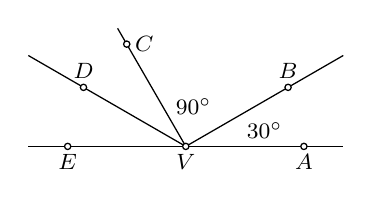
\begin{tikzpicture}
                        % \clip (0,0) rectangle (14.000000,10.000000);
                        {\footnotesize

                        % Marking point V by circle
                        \draw [line width=0.016cm] (4.000000,1.500000) circle (0.040000);%
                        \draw (4.000000,1.500000) node [anchor=north] { $V$ };%

                        % Marking point A by circle
                        \draw [line width=0.016cm] (5.500000,1.500000) circle (0.040000);%
                        \draw (5.500000,1.500000) node [anchor=north] { $A$ };%

                        % Marking point E by circle
                        \draw [line width=0.016cm] (2.500000,1.500000) circle (0.040000);%
                        \draw (2.500000,1.500000) node [anchor=north] { $E$ };%

                        % Drawing line A E
                        \draw [line width=0.016cm] (2.000000,1.500000) -- (2.460000,1.500000);%
                        \draw [line width=0.016cm] (2.540000,1.500000) -- (3.960000,1.500000);%
                        \draw [line width=0.016cm] (4.040000,1.500000) -- (5.460000,1.500000);%
                        \draw [line width=0.016cm] (5.540000,1.500000) -- (6.000000,1.500000);%

                        % Marking point B by circle
                        \draw [line width=0.016cm] (5.299038,2.250000) circle (0.040000);%
                        \draw (5.299038,2.250000) node [anchor=south] { $B$ };%

                        % Marking point C by circle
                        \draw [line width=0.016cm] (3.250000,2.799038) circle (0.040000);%
                        \draw (3.250000,2.799038) node [anchor=west] { $C$ };%

                        % Marking point D by circle
                        \draw [line width=0.016cm] (2.700962,2.250000) circle (0.040000);%
                        \draw (2.700962,2.250000) node [anchor=south] { $D$ };%

                        % Drawing line V D
                        % \draw [line width=0.016cm] (4.519615,1.200000) -- (4.034641,1.480000);%
                        \draw [line width=0.016cm] (3.965359,1.520000) -- (2.735603,2.230000);%
                        \draw [line width=0.016cm] (2.666321,2.270000) -- (2.000000,2.654701);%

                        % Drawing line V C
                        % \draw [line width=0.016cm] (4.173205,1.200000) -- (4.020000,1.465359);%
                        \draw [line width=0.016cm] (3.980000,1.534641) -- (3.270000,2.764397);%
                        \draw [line width=0.016cm] (3.230000,2.833679) -- (3.133975,3.000000);%

                        % Drawing line V B
                        % \draw [line width=0.016cm] (3.480385,1.200000) -- (3.965359,1.480000);%
                        \draw [line width=0.016cm] (4.034641,1.520000) -- (5.264397,2.230000);%
                        \draw [line width=0.016cm] (5.333679,2.270000) -- (6.000000,2.654700);%

                        % Marking point {30^\circ}
                        \draw (5.000000,1.500000) node [anchor=south] { ${30^\circ}$ };%

                        % Marking point {90^\circ}
                        \draw (4.100000,1.800000) node [anchor=south] { ${90^\circ}$ };%
                        }
                    \end{tikzpicture}

                \end{figure}
            \end{exampleblock}}
        \end{frame}





%%%%%%%%%%%%%%%%%%%%%%%%%%%%%%%%%%

    \subsection{Vzporednost in pravokotnost}

        \begin{frame}
            \frametitle{Vzporednost}
            
            \begin{alertblock}{Aksiom o vzporednici}
                Skozi izbrano točko, ki ne leži na premici, lahko tej premici načrtamo natanko eno vzporednico.

                \begin{figure}[H]
                    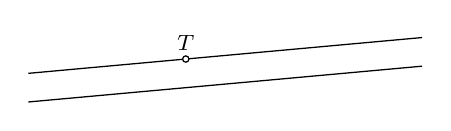
\begin{tikzpicture}
                    % \clip (0,0) rectangle (14.000000,10.000000);
                    {\footnotesize

                    % Drawing line p
                    \draw [line width=0.016cm] (1.000000,1.454545) -- (6.000000,1.909091);%

                    % Drawing line q
                    \draw [line width=0.016cm] (1.000000,1.818182) -- (2.960164,1.996379);%
                    \draw [line width=0.016cm] (3.039836,2.003621) -- (6.000000,2.272727);%

                    % Marking point T by circle
                    \draw [line width=0.016cm] (3.000000,2.000000) circle (0.040000);%
                    \draw (3.000000,2.000000) node [anchor=south] { $T$ };%
                    }
                    \end{tikzpicture}

                \end{figure}

            \end{alertblock}

            \begin{block}{}
                \textbf{Vzporednost} je v množici premic na ravnini \textit{ekvivalenčna relacija}, saj je:
                \begin{itemize}
                    \item \textit{refleksivna}: $p\parallel p$ -- vsaka premica je vzporedna sama sebi;
                    \item \textit{simetrična}: $p\parallel q \Rightarrow q\parallel p$ -- če je premica $p$ vzporedna premici $q$, je tudi premica $q$ vzporedna premici $p$;
                    \item \textit{tranzitivna}: $p\parallel q \land q \parallel r \rightarrow p \parallel r$ -- če je premica $p$ vzporedna premici $q$, premica $q$ pa vzporedna premici $r$, 
                        je tudi premica $p$ vzporedna premici $r$.
                \end{itemize}
            \end{block}

        \end{frame}

        
        \begin{frame}
            \begin{block}{}
                Če vzporednici sekamo s premico, dobimo dve presečišči, ob njiju pa pare \textbf{kotov z vzporednimi kraki}:
                
                \begin{figure}[H]
                    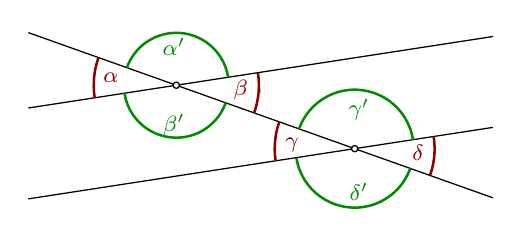
\begin{tikzpicture}
                    % \clip (0,0) rectangle (14.000000,10.000000);
                    {\footnotesize

                    % Drawing line p
                    \draw [line width=0.016cm] (1.300000,1.315385) -- (5.405096,1.946938);%
                    \draw [line width=0.016cm] (5.484166,1.959102) -- (7.200000,2.223077);%

                    % Drawing line q
                    \draw [line width=0.016cm] (1.300000,2.469231) -- (3.139995,2.752307);%
                    \draw [line width=0.016cm] (3.219065,2.764472) -- (7.200000,3.376923);%

                    % Drawing line r
                    \draw [line width=0.016cm] (1.300000,3.426667) -- (3.141842,2.771790);%
                    \draw [line width=0.016cm] (3.217219,2.744989) -- (5.406942,1.966421);%
                    \draw [line width=0.016cm] (5.482319,1.939620) -- (7.200000,1.328889);%

                    % Marking point U by circle
                    \draw [line width=0.016cm] (5.444631,1.953020) circle (0.040000);%

                    % Marking point V by circle
                    \draw [line width=0.016cm] (3.179530,2.758389) circle (0.040000);%

                    % Changing color 139 0 0
                    \definecolor{r139g0b0}{rgb}{0.545098,0.000000,0.000000}%
                    \color{r139g0b0}% 

                    % Drawing arc V L 28.32
                    \draw [line width=0.032cm] (2.191446,3.109708) -- (2.187982,3.099807) arc (161:188:1.048682 and 1.048682) -- (2.143042,2.598930);%

                    % Drawing arc V M 28.32
                    \draw [line width=0.032cm] (4.167614,2.407070) -- (4.171079,2.416971) arc (341:360:1.048682 and 1.048682) --(4.228212,2.758389) arc (0:8:1.048682 and 1.048682) -- (4.216018,2.917849);%

                    % Drawing arc U N 28.32
                    \draw [line width=0.032cm] (4.487996,2.293157) -- (4.484642,2.283571) arc (161:188:1.015305 and 1.015305) -- (4.441133,1.798636);%

                    % Drawing arc U O 28.32
                    \draw [line width=0.032cm] (6.401266,1.612883) -- (6.404620,1.622469) arc (341:360:1.015305 and 1.015305) --(6.459935,1.953020) arc (0:8:1.015305 and 1.015305) -- (6.448129,2.107404);%

                    % Marking point \alpha
                    \draw (2.350000,2.850000) node  { $\alpha$ };%

                    % Marking point \beta
                    \draw (4.000000,2.700000) node  { $\beta$ };%

                    % Marking point \gamma
                    \draw (4.650000,2.000000) node  { $\gamma$ };%

                    % Marking point \delta
                    \draw (6.250000,1.900000) node  { $\delta$ };%

                    % Changing color 0 139 0
                    \definecolor{r0g139b0}{rgb}{0.000000,0.545098,0.000000}%
                    \color{r0g139b0}% 

                    % Drawing arc V J 151.68
                    \draw [line width=0.032cm] (3.837639,2.859637) -- (3.837184,2.862551) arc (9:160:0.665852 and 0.665852) -- (2.552155,2.981456);%

                    % Drawing arc V K 151.68
                    \draw [line width=0.032cm] (2.521421,2.657142) -- (2.521876,2.654227) arc (189:340:0.665852 and 0.665852) -- (3.806905,2.535322);%

                    % Drawing arc U P 151.68
                    \draw [line width=0.032cm] (6.184950,2.066915) -- (6.184438,2.070194) arc (9:160:0.749029 and 0.749029) -- (4.738885,2.203952);%

                    % Drawing arc U R 151.68
                    \draw [line width=0.032cm] (4.704312,1.839125) -- (4.704824,1.835846) arc (189:340:0.749029 and 0.749029) -- (6.150377,1.702088);%

                    % Marking point \alpha'
                    \draw (3.150000,3.250000) node  { $\alpha'$ };%

                    % Marking point \beta'
                    \draw (3.150000,2.250000) node  { $\beta'$ };%

                    % Marking point \gamma'
                    \draw (5.500000,2.450000) node  { $\gamma'$ };%

                    % Marking point \delta'
                    \draw (5.500000,1.400000) node  { $\delta'$ };%
                    \color{black}
                    }
                    \end{tikzpicture}
                    
                \end{figure}

                \begin{itemize}
                    \item pari kotov $(\alpha, \gamma)$, $(\beta, \delta)$, $(\alpha', \gamma')$, $(\beta', \delta')$ imajo oba kraka vzporedna v isto smer;
                    \item pari kotov z istim vrhom $(\alpha, \beta)$; $(\gamma, \delta)$, $(\alpha', \beta')$; $(\gamma', \delta')$ imajo oba kraka vzporedna v nasprotno smer -- \textbf{sovršni koti};
                    \item pari kotov $(\alpha, \alpha')$, $(\beta, \beta')$, $(\gamma,\gamma')$, $(\delta,\delta')$ imajo en krak vzporeden v isto smer, drugi krak pa vzporeden v nasprotno smer.
                \end{itemize}
            \end{block}
        \end{frame}


        \begin{frame}
            \begin{block}{Izrek}
                Para konveksnih kotov z vzporednimi kraki sta bodisi skladna bodisi suplementarna.

                \begin{figure}[H]
                    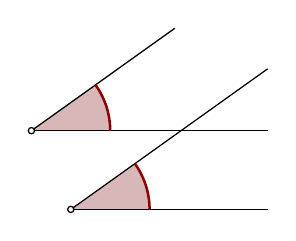
\begin{tikzpicture}
                    % \clip (0,0) rectangle (14.000000,10.000000);
                    {\footnotesize

                    % Changing color 215 183 183
                    \definecolor{r215g183b183}{rgb}{0.843137,0.717647,0.717647}%
                    \color{r215g183b183}% 

                    % Filling circle arc V D 35.54
                    \fill (1.500000,2.500000) -- (2.500000,2.500000) arc (0:35:1.000000 and 1.000000) -- (2.313733,3.081238) -- cycle;%

                    % Filling circle arc U E 35.54
                    \fill (2.000000,1.500000) -- (3.000000,1.500000) arc (0:35:1.000000 and 1.000000) -- (2.813733,2.081238) -- cycle;%

                    % Changing color 0 0 0
                    \definecolor{r0g0b0}{rgb}{0.000000,0.000000,0.000000}%
                    \color{r0g0b0}% 

                    % Marking point V by circle
                    \draw [line width=0.016cm] (1.500000,2.500000) circle (0.040000);%

                    % Drawing line V A
                    % \draw [line width=0.016cm] (1.000000,2.500000) -- (1.460000,2.500000);%
                    \draw [line width=0.016cm] (1.540000,2.500000) -- (4.500000,2.500000);%

                    % Drawing line V B
                    \draw [line width=0.016cm] (3.320000,3.800000) -- (1.532549,2.523250);%
                    % \draw [line width=0.016cm] (1.467451,2.476750) -- (1.000000,2.142857);%

                    % Marking point U by circle
                    \draw [line width=0.016cm] (2.000000,1.500000) circle (0.040000);%

                    % Drawing line r
                    % \draw [line width=0.016cm] (1.300000,1.000000) -- (1.967451,1.476750);%
                    \draw [line width=0.016cm] (2.032549,1.523250) -- (4.500000,3.285714);%

                    % Drawing line s
                    % \draw [line width=0.016cm] (1.000000,1.500000) -- (1.960000,1.500000);%
                    \draw [line width=0.016cm] (2.040000,1.500000) -- (4.500000,1.500000);%

                    % Changing color 139 0 0
                    \definecolor{r139g0b0}{rgb}{0.545098,0.000000,0.000000}%
                    \color{r139g0b0}% 

                    % Drawing arc V D 35.54
                    \draw [line width=0.032cm] (2.500000,2.500000) arc (360:360:1.000000 and 1.000000) --(2.500000,2.500000) arc (0:35:1.000000 and 1.000000) -- (2.313733,3.081238);%

                    % Drawing arc U E 35.54
                    \draw [line width=0.032cm] (3.000000,1.500000) arc (360:360:1.000000 and 1.000000) --(3.000000,1.500000) arc (0:35:1.000000 and 1.000000) -- (2.813733,2.081238);%
                    \color{black}
                    }
                    \end{tikzpicture} ~~~~
                    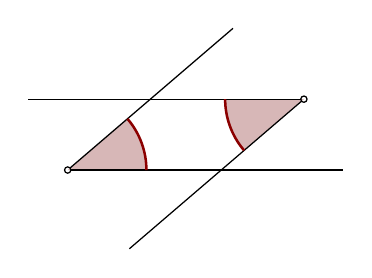
\begin{tikzpicture}
                    % \clip (0,0) rectangle (14.000000,10.000000);
                    {\footnotesize

                    % Changing color 215 183 183
                    \definecolor{r215g183b183}{rgb}{0.843137,0.717647,0.717647}%
                    \color{r215g183b183}% 

                    % Filling circle arc V D 40.60
                    \fill (1.500000,2.000000) -- (2.500000,2.000000) arc (0:40:1.000000 and 1.000000) -- (2.259257,2.650791) -- cycle;%

                    % Filling circle arc U E 40.60
                    \fill (4.500000,2.900000) -- (3.500000,2.900000) arc (180:220:1.000000 and 1.000000) -- (3.740743,2.249209) -- cycle;%

                    % Changing color 0 0 0
                    \definecolor{r0g0b0}{rgb}{0.000000,0.000000,0.000000}%
                    \color{r0g0b0}% 

                    % Marking point V by circle
                    \draw [line width=0.016cm] (1.500000,2.000000) circle (0.040000);%

                    % Drawing line V A
                    % \draw [line width=0.016cm] (1.000000,2.000000) -- (1.460000,2.000000);%
                    \draw [line width=0.016cm] (1.540000,2.000000) -- (5.000000,2.000000);%

                    % Drawing line V B
                    \draw [line width=0.016cm] (3.600000,3.800000) -- (1.530370,2.026032);%
                    % \draw [line width=0.016cm] (1.469630,1.973968) -- (1.000000,1.571429);%

                    % Marking point U by circle
                    \draw [line width=0.016cm] (4.500000,2.900000) circle (0.040000);%

                    % Drawing line r
                    \draw [line width=0.016cm] (2.283333,1.000000) -- (4.469630,2.873968);%
                    % \draw [line width=0.016cm] (4.530370,2.926032) -- (5.000000,3.328571);%

                    % Drawing line s
                    \draw [line width=0.016cm] (1.000000,2.900000) -- (4.460000,2.900000);%
                    % \draw [line width=0.016cm] (4.540000,2.900000) -- (5.000000,2.900000);%

                    % Changing color 139 0 0
                    \definecolor{r139g0b0}{rgb}{0.545098,0.000000,0.000000}%
                    \color{r139g0b0}% 

                    % Drawing arc V D 40.60
                    \draw [line width=0.032cm] (2.500000,2.000000) arc (360:360:1.000000 and 1.000000) --(2.500000,2.000000) arc (0:40:1.000000 and 1.000000) -- (2.259257,2.650791);%

                    % Drawing arc U E 40.60
                    \draw [line width=0.032cm] (3.500000,2.900000) arc (180:220:1.000000 and 1.000000) -- (3.740743,2.249209);%
                    \color{black}
                    }
                    \end{tikzpicture} ~~~~
                    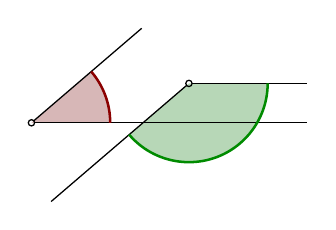
\begin{tikzpicture}
                    % \clip (0,0) rectangle (14.000000,10.000000);
                    {\footnotesize

                    % Changing color 215 183 183
                    \definecolor{r215g183b183}{rgb}{0.843137,0.717647,0.717647}%
                    \color{r215g183b183}% 

                    % Filling circle arc V D 40.60
                    \fill (1.500000,2.000000) -- (2.500000,2.000000) arc (0:40:1.000000 and 1.000000) -- (2.259257,2.650791) -- cycle;%

                    % Changing color 183 215 183
                    \definecolor{r183g215b183}{rgb}{0.717647,0.843137,0.717647}%
                    \color{r183g215b183}% 

                    % Filling circle arc U G 139.40
                    \fill (3.500000,2.500000) -- (2.740743,1.849209) -- (2.745290,1.843941) arc (221:360:1.000000 and 1.000000) --(4.500000,2.500000) arc (0:0:1.000000 and 1.000000) -- cycle;%

                    % Changing color 0 0 0
                    \definecolor{r0g0b0}{rgb}{0.000000,0.000000,0.000000}%
                    \color{r0g0b0}% 

                    % Marking point V by circle
                    \draw [line width=0.016cm] (1.500000,2.000000) circle (0.040000);%

                    % Drawing line V A
                    % \draw [line width=0.016cm] (1.000000,2.000000) -- (1.460000,2.000000);%
                    \draw [line width=0.016cm] (1.540000,2.000000) -- (5.000000,2.000000);%

                    % Drawing line V B
                    \draw [line width=0.016cm] (2.900000,3.200000) -- (1.530370,2.026032);%
                    % \draw [line width=0.016cm] (1.469630,1.973968) -- (1.000000,1.571429);%

                    % Marking point U by circle
                    \draw [line width=0.016cm] (3.500000,2.500000) circle (0.040000);%

                    % Drawing line r
                    \draw [line width=0.016cm] (1.750000,1.000000) -- (3.469630,2.473968);%
                    % \draw [line width=0.016cm] (3.530370,2.526032) -- (4.316667,3.200000);%

                    % Drawing line s
                    % \draw [line width=0.016cm] (1.000000,2.500000) -- (3.460000,2.500000);%
                    \draw [line width=0.016cm] (3.540000,2.500000) -- (5.000000,2.500000);%

                    % Changing color 139 0 0
                    \definecolor{r139g0b0}{rgb}{0.545098,0.000000,0.000000}%
                    \color{r139g0b0}% 

                    % Drawing arc V D 40.60
                    \draw [line width=0.032cm] (2.500000,2.000000) arc (360:360:1.000000 and 1.000000) --(2.500000,2.000000) arc (0:40:1.000000 and 1.000000) -- (2.259257,2.650791);%

                    % Changing color 0 139 0
                    \definecolor{r0g139b0}{rgb}{0.000000,0.545098,0.000000}%
                    \color{r0g139b0}% 

                    % Drawing arc U G 139.40
                    \draw [line width=0.032cm] (2.740743,1.849209) -- (2.745290,1.843941) arc (221:360:1.000000 and 1.000000);%
                    \color{black}
                    }
                    \end{tikzpicture}

                \end{figure}
            \end{block}

            \begin{block}{}
                Sovršna kota sta skladna -- imata isti sokot.

                \begin{figure}[H]
                    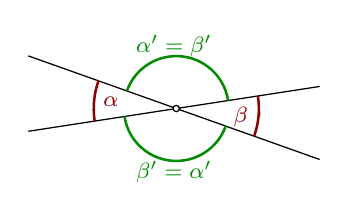
\begin{tikzpicture}
                    % \clip (0,0) rectangle (14.000000,10.000000);
                    {\footnotesize

                    % Drawing line p

                    % Drawing line q
                    \draw [line width=0.016cm] (1.300000,2.469231) -- (3.139995,2.752307);%
                    \draw [line width=0.016cm] (3.219065,2.764472) -- (5.000000,3.038462);%

                    % Drawing line r
                    \draw [line width=0.016cm] (1.300000,3.426667) -- (3.141842,2.771790);%
                    \draw [line width=0.016cm] (3.217219,2.744989) -- (5.000000,2.111111);%

                    % Marking point U by circle

                    % Marking point V by circle
                    \draw [line width=0.016cm] (3.179530,2.758389) circle (0.040000);%

                    % Changing color 139 0 0
                    \definecolor{r139g0b0}{rgb}{0.545098,0.000000,0.000000}%
                    \color{r139g0b0}% 

                    % Drawing arc V L 28.32
                    \draw [line width=0.032cm] (2.191446,3.109708) -- (2.187982,3.099807) arc (161:188:1.048682 and 1.048682) -- (2.143042,2.598930);%

                    % Drawing arc V M 28.32
                    \draw [line width=0.032cm] (4.167614,2.407070) -- (4.171079,2.416971) arc (341:360:1.048682 and 1.048682) --(4.228212,2.758389) arc (0:8:1.048682 and 1.048682) -- (4.216018,2.917849);%

                    % Marking point \alpha
                    \draw (2.350000,2.850000) node  { $\alpha$ };%

                    % Marking point \beta
                    \draw (4.000000,2.650000) node  { $\beta$ };%

                    % Changing color 0 139 0
                    \definecolor{r0g139b0}{rgb}{0.000000,0.545098,0.000000}%
                    \color{r0g139b0}% 

                    % Drawing arc V J 151.68
                    \draw [line width=0.032cm] (3.837639,2.859637) -- (3.837184,2.862551) arc (9:160:0.665852 and 0.665852) -- (2.552155,2.981456);%

                    % Drawing arc V K 151.68
                    \draw [line width=0.032cm] (2.521421,2.657142) -- (2.521876,2.654227) arc (189:340:0.665852 and 0.665852) -- (3.806905,2.535322);%

                    % Marking point \alpha'
                    \draw (3.150000,3.55000) node  { $\alpha'=\beta'$ };%

                    % Marking point \beta'
                    \draw (3.150000,1.95000) node  { $\beta'=\alpha'$ };%
                    \color{black}
                    }
                    \end{tikzpicture}
                \end{figure}
            \end{block}
        \end{frame}


        \begin{frame}
            \frametitle{Pravokotnost}

            \begin{alertblock}{Definicija}
                \textbf{Pravokotnica} je premica, ki dano premico seka pod pravim kotom.
            \end{alertblock}

            \begin{block}{Izrek}
                Skozi izbrano točko lahko na dano premico načrtamo natanko eno pravokotnico.
            
                \begin{figure}[H]
                    \begin{tikzpicture}
                        % \clip (0,0) rectangle (14.000000,10.000000);
                        {\footnotesize

                        % Drawing line a
                        \draw [line width=0.016cm] (1.000000,1.428571) -- (5.500000,2.071429);%

                        % Drawing line b
                        \draw [line width=0.016cm] (3.357143,1.000000) -- (3.005657,3.460402);%
                        \draw [line width=0.016cm] (2.994343,3.539598) -- (2.928571,4.000000);%

                        % Marking point T by circle
                        \draw [line width=0.016cm] (3.000000,3.500000) circle (0.040000);%
                        \draw (3.000000,3.500000) node [anchor=west] { $T$ };%
                        }
                    \end{tikzpicture}

                \end{figure}
            \end{block}
        \end{frame}


        \begin{frame}
            \begin{block}{}
                \textbf{Kota s pravokotnimi kraki} sta konveksna kota, katerih nosilki krakov enega kota sta pravokotni na nosilki krakov drugega kota.
            \end{block}

            \begin{block}{Izrek}
                Para konveksnih kotov s pravokotnimi kraki sta bodisi skladna bodisi suplementarna.

                \begin{figure}[H]
                    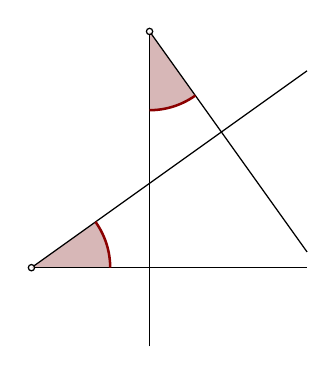
\begin{tikzpicture}
                        % \clip (0,0) rectangle (14.000000,10.000000);
                        {\footnotesize

                        % Changing color 215 183 183
                        \definecolor{r215g183b183}{rgb}{0.843137,0.717647,0.717647}%
                        \color{r215g183b183}% 

                        % Filling circle arc V D 35.54
                        \fill (1.500000,2.000000) -- (2.500000,2.000000) arc (0:35:1.000000 and 1.000000) -- (2.313733,2.581238) -- cycle;%

                        % Filling circle arc U E 35.54
                        \fill (3.000000,5.000000) -- (3.000000,4.000000) -- (3.000000,4.000000) arc (270:305:1.000000 and 1.000000) -- (3.581238,4.186266) -- cycle;%

                        % Changing color 0 0 0
                        \definecolor{r0g0b0}{rgb}{0.000000,0.000000,0.000000}%
                        \color{r0g0b0}% 

                        % Marking point V by circle
                        \draw [line width=0.016cm] (1.500000,2.000000) circle (0.040000);%

                        % Drawing line V A
                        % \draw [line width=0.016cm] (1.000000,2.000000) -- (1.460000,2.000000);%
                        \draw [line width=0.016cm] (1.540000,2.000000) -- (5.000000,2.000000);%

                        % Drawing line V B
                        % \draw [line width=0.016cm] (1.000000,1.642857) -- (1.467451,1.976750);%
                        \draw [line width=0.016cm] (1.532549,2.023250) -- (5.000000,4.500000);%

                        % Marking point U by circle
                        \draw [line width=0.016cm] (3.000000,5.000000) circle (0.040000);%

                        % Drawing line r
                        % \draw [line width=0.016cm] (2.642857,5.500000) -- (2.976750,5.032549);%
                        \draw [line width=0.016cm] (3.023250,4.967451) -- (5.000000,2.200000);%

                        % Drawing line s
                        \draw [line width=0.016cm] (3.000000,1.000000) -- (3.000000,4.960000);%
                        % \draw [line width=0.016cm] (3.000000,5.040000) -- (3.000000,5.500000);%

                        % Changing color 139 0 0
                        \definecolor{r139g0b0}{rgb}{0.545098,0.000000,0.000000}%
                        \color{r139g0b0}% 

                        % Drawing arc V D 35.54
                        \draw [line width=0.032cm] (2.500000,2.000000) arc (360:360:1.000000 and 1.000000) --(2.500000,2.000000) arc (0:35:1.000000 and 1.000000) -- (2.313733,2.581238);%

                        % Drawing arc U E 35.54
                        \draw [line width=0.032cm] (3.000000,4.000000) -- (3.000000,4.000000) arc (270:305:1.000000 and 1.000000) -- (3.581238,4.186266);%
                        \color{black}
                        }
                    \end{tikzpicture} ~~~~~~~~~~
                    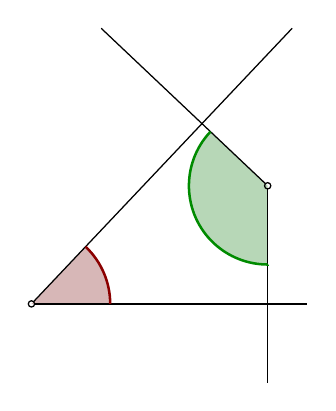
\begin{tikzpicture}
                        % \clip (0,0) rectangle (14.000000,10.000000);
                        {\footnotesize

                        % Changing color 215 183 183
                        \definecolor{r215g183b183}{rgb}{0.843137,0.717647,0.717647}%
                        \color{r215g183b183}% 

                        % Filling circle arc V D 46.59
                        \fill (1.500000,2.000000) -- (2.500000,2.000000) arc (0:46:1.000000 and 1.000000) -- (2.187200,2.726468) -- cycle;%

                        % Changing color 183 215 183
                        \definecolor{r183g215b183}{rgb}{0.717647,0.843137,0.717647}%
                        \color{r183g215b183}% 

                        % Filling circle arc U F 133.41
                        \fill (4.500000,3.500000) -- (3.773532,4.187200) -- (3.768646,4.181998) arc (137:270:1.000000 and 1.000000) -- (4.500000,2.500000) -- cycle;%

                        % Changing color 0 0 0
                        \definecolor{r0g0b0}{rgb}{0.000000,0.000000,0.000000}%
                        \color{r0g0b0}% 

                        % Marking point V by circle
                        \draw [line width=0.016cm] (1.500000,2.000000) circle (0.040000);%

                        % Drawing line V A
                        % \draw [line width=0.016cm] (1.000000,2.000000) -- (1.460000,2.000000);%
                        \draw [line width=0.016cm] (1.540000,2.000000) -- (5.000000,2.000000);%

                        % Drawing line V B
                        \draw [line width=0.016cm] (4.810811,5.500000) -- (1.527488,2.029059);%
                        % \draw [line width=0.016cm] (1.472512,1.970941) -- (1.000000,1.471429);%

                        % Marking point U by circle
                        \draw [line width=0.016cm] (4.500000,3.500000) circle (0.040000);%

                        % Drawing line r
                        \draw [line width=0.016cm] (2.385714,5.500000) -- (4.470941,3.527488);%
                        % \draw [line width=0.016cm] (4.529059,3.472512) -- (5.000000,3.027027);%

                        % Drawing line s
                        \draw [line width=0.016cm] (4.500000,1.000000) -- (4.500000,3.460000);%
                        % \draw [line width=0.016cm] (4.500000,3.540000) -- (4.500000,5.500000);%

                        % Changing color 139 0 0
                        \definecolor{r139g0b0}{rgb}{0.545098,0.000000,0.000000}%
                        \color{r139g0b0}% 

                        % Drawing arc V D 46.59
                        \draw [line width=0.032cm] (2.500000,2.000000) arc (360:360:1.000000 and 1.000000) --(2.500000,2.000000) arc (0:46:1.000000 and 1.000000) -- (2.187200,2.726468);%

                        % Changing color 0 139 0
                        \definecolor{r0g139b0}{rgb}{0.000000,0.545098,0.000000}%
                        \color{r0g139b0}% 

                        % Drawing arc U F 133.41
                        \draw [line width=0.032cm] (3.773532,4.187200) -- (3.768646,4.181998) arc (137:270:1.000000 and 1.000000) -- (4.500000,2.500000);%
                        \color{black}
                        }
                    \end{tikzpicture}

                \end{figure}
            \end{block}
        \end{frame}


        \begin{frame}


            \begin{columns}
                \column{0.63\textwidth}
                    \begin{alertblock}{Definicija}
                        \textbf{Pravokotna projekcija} točke $T$ na premico $p$ je točka $T'$, 
                        ki leži na presečišču premice $p$ in pravokotnice $q$ skozi točko $T$ na premico $p$. \\
                        Točka $T'$ je točki $T$ najbližja točka premice $p$. 
                    \end{alertblock}
                    
                    \begin{block}{}
                        \textbf{Razdalja} točke $T$ od premice $p$ je: $$d(T,p)=d(T,T')=\left\lvert TT'\right\rvert.$$
                    \end{block} 

                \column{0.35\textwidth}            
                    % \begin{figure}
                    % 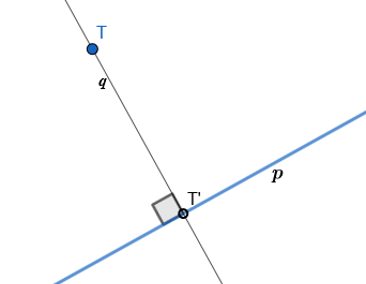
\includegraphics[scale=0.5]{Slike in skice/Pravokotna_projekcija.png}
                    % \end{figure}
                \begin{block}{}
                    \begin{figure}[H]
                        \begin{tikzpicture}
                            % \clip (0,0) rectangle (14.000000,10.000000);
                            {\footnotesize
                            
                            % Drawing line Q
                            \draw [line width=0.016cm] (3.000000,1.000000) -- (2.932918,1.134164);%
                            \draw [line width=0.016cm] (2.899377,1.201246) -- (2.832295,1.335410);%
                            \draw [line width=0.016cm] (2.798754,1.402492) -- (2.731672,1.536656);%
                            \draw [line width=0.016cm] (2.698131,1.603738) -- (2.631049,1.737902);%
                            \draw [line width=0.016cm] (2.582111,1.835777) -- (2.530426,1.939149);%
                            \draw [line width=0.016cm] (2.496885,2.006231) -- (2.429803,2.140395);%
                            \draw [line width=0.016cm] (2.396262,2.207477) -- (2.329180,2.341641);%
                            \draw [line width=0.016cm] (2.295639,2.408723) -- (2.228557,2.542887);%
                            \draw [line width=0.016cm] (2.195016,2.609969) -- (2.127933,2.744133);%
                            \draw [line width=0.016cm] (2.094392,2.811215) -- (2.027310,2.945379);%
                            \draw [line width=0.016cm] (1.993769,3.012461) -- (1.926687,3.146625);%
                            \draw [line width=0.016cm] (1.893146,3.213707) -- (1.826064,3.347871);%
                            \draw [line width=0.016cm] (1.792523,3.414953) -- (1.725441,3.549117);%
                            \draw [line width=0.016cm] (1.691900,3.616200) -- (1.624818,3.750364);%
                            \draw [line width=0.016cm] (1.591277,3.817446) -- (1.524195,3.951610);%
                            \draw [line width=0.016cm] (1.482111,4.035777) -- (1.423572,4.152856);%
                            \draw [line width=0.016cm] (1.390031,4.219938) -- (1.322949,4.354102);%
                            \draw [line width=0.016cm] (1.289408,4.421184) -- (1.250000,4.500000);%
                            
                            % Marking point q
                            \draw (1.847000,3.306000) node [anchor=east] { $q$ };%
                            
                            % Marking point T by circle
                            \draw [line width=0.016cm] (1.500000,4.000000) circle (0.040000);%
                            \draw (1.550000,4.000000) node [anchor=south] { $T$ };%
                            
                            % Marking point \frac{\pi}{2}
                            \draw (2.250000,2.000000) node  { $\frac{\pi}{2}$ };%
                            
                            % Changing color 0 0 255
                            \definecolor{r0g0b255}{rgb}{0.000000,0.000000,1.000000}%
                            \color{r0g0b255}% 
                            
                            % Drawing line P
                            \draw [line width=0.016cm] (1.000000,1.000000) -- (2.564223,1.782111);%
                            \draw [line width=0.016cm] (2.635777,1.817889) -- (4.500000,2.750000);%
                            
                            % Marking point p
                            \draw (4.155000,2.578000) node [anchor=north] { $p$ };%
                            
                            % Changing color 255 0 0
                            \definecolor{r255g0b0}{rgb}{1.000000,0.000000,0.000000}%
                            \color{r255g0b0}% 
                            
                            % Marking point T' by circle
                            \draw [line width=0.016cm] (2.600000,1.800000) circle (0.040000);%
                            \draw (2.500000,1.900000) node [anchor=south west] { $T'$ };%
                            \color{black}
                            }
                        \end{tikzpicture}
                    \end{figure}
                \end{block}
            \end{columns}

            \begin{block}{}
                Pravokotna projekcija daljice $AB$ na premico je daljica $A'B'$, katere krajišči sta pravokotni projekciji točk $A$ in $B$.
            \end{block}

            % \note{
            %     TABLA: konstrukcija pravokotne projekcije točke  z ravnilom in šestilom
            %     \\
            %     TABLA: konstruckija pravokotne projekcije daljice z ravnilom in šestilom
            % }


        \end{frame}


        \begin{frame}
            \frametitle{Toge preslikave}
            
            \begin{alertblock}{Definicija}
                \textbf{Toga preslikava} (izometrija) je preslikava v ravnini, ki ohranja razdalje.
                \begin{align*}
                    \tau:~ &A \mapsto A' \\ 
                    \tau:~ &B \mapsto B' \\ 
                    d(A,B)&=d(A',B')
                \end{align*}
            \end{alertblock}

            \begin{block}{}
                Med toge preslikave spadajo:
                    \begin{itemize}
                        \item \textbf{vzporedni premiki};
                        \item \textbf{zrcaljenje preko premice/premice};
                        \item \textbf{rotacija okoli točke}.
                    \end{itemize}

                Če kombiniramo več togih preslikav, je dobljena preslikava spet toga preslikava.
            \end{block}

        \end{frame}


        \begin{frame}

            \begin{block}{}
                \textbf{Vzporedni premik} ali \textbf{translacija} za dano usmerjeno daljico $\overrightarrow{MN}$ preslika točko $T$ v tako točko $T'$, da sta daljici $TT'$ in $MN$ enako dolgi, vzporedni in enako usmerjeni. \\  %(vektorja $\overrightarrow{TT'}$ in $\overrightarrow{AB}$ sta enaka). \\
                
                % \begin{figure}
                %     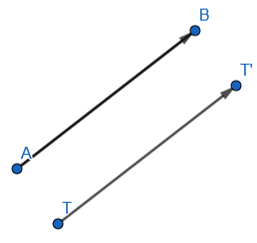
\includegraphics[scale=0.5]{Slike in skice/Vzporedni_premik_tocke.png}
                %     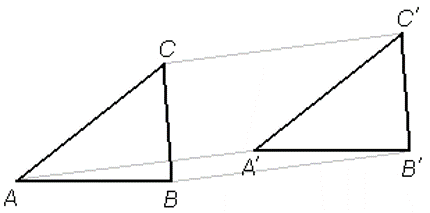
\includegraphics[scale=0.5]{Slike in skice/Vzporedni_premik_trikotnika.png}
                % \end{figure}

                \begin{figure}[H]
                    \begin{tikzpicture}
                        % \clip (0,0) rectangle (14.000000,10.000000);
                        {\footnotesize
                        
                        % Drawing segment M N
                        \draw [line width=0.016cm] (1.537947,2.512649) -- (4.462053,3.487351);%
                        
                        % Drawing arrow M N 1.00
                        \draw [line width=0.016cm] (4.205447,3.443092) -- (4.460726,3.492412);%
                        \draw [line width=0.016cm] (4.205447,3.443092) -- (4.405943,3.468648);%
                        \draw [line width=0.016cm] (4.230213,3.368795) -- (4.464028,3.482506);%
                        \draw [line width=0.016cm] (4.230213,3.368795) -- (4.405943,3.468648);%
                        
                        % Drawing segment T T'
                        \draw [line width=0.016cm] (2.037947,1.512649) -- (2.142302,1.547434);%
                        \draw [line width=0.016cm] (2.213454,1.571151) -- (2.355756,1.618585);%
                        \draw [line width=0.016cm] (2.426907,1.642302) -- (2.569210,1.689737);%
                        \draw [line width=0.016cm] (2.640361,1.713454) -- (2.782664,1.760888);%
                        \draw [line width=0.016cm] (2.853815,1.784605) -- (2.996117,1.832039);%
                        \draw [line width=0.016cm] (3.067269,1.855756) -- (3.209571,1.903190);%
                        \draw [line width=0.016cm] (3.280722,1.926907) -- (3.423025,1.974342);%
                        \draw [line width=0.016cm] (3.494176,1.998059) -- (3.636479,2.045493);%
                        \draw [line width=0.016cm] (3.707630,2.069210) -- (3.849932,2.116644);%
                        \draw [line width=0.016cm] (3.921084,2.140361) -- (4.063386,2.187795);%
                        \draw [line width=0.016cm] (4.134537,2.211512) -- (4.276840,2.258947);%
                        \draw [line width=0.016cm] (4.347991,2.282664) -- (4.490294,2.330098);%
                        \draw [line width=0.016cm] (4.561445,2.353815) -- (4.703747,2.401249);%
                        \draw [line width=0.016cm] (4.774899,2.424966) -- (4.917201,2.472400);%
                        
                        % Drawing arrow T T' 1.00
                        \draw [line width=0.016cm] (4.705447,2.443092) -- (4.960726,2.492412);%
                        \draw [line width=0.016cm] (4.705447,2.443092) -- (4.905943,2.468648);%
                        \draw [line width=0.016cm] (4.730213,2.368795) -- (4.964028,2.482506);%
                        \draw [line width=0.016cm] (4.730213,2.368795) -- (4.905943,2.468648);%
                        
                        % Marking point T by circle
                        \draw [line width=0.016cm] (2.000000,1.500000) circle (0.040000);%
                        \draw (2.000000,1.500000) node [anchor=north] { $T$ };%
                        
                        % Marking point A by circle
                        \draw [line width=0.016cm] (6.000000,2.000000) circle (0.040000);%
                        \draw (6.000000,2.000000) node [anchor=north] { $A$ };%
                        
                        % Marking point B by circle
                        \draw [line width=0.016cm] (9.000000,2.000000) circle (0.040000);%
                        \draw (9.000000,2.000000) node [anchor=north] { $B$ };%
                        
                        % Marking point C by circle
                        \draw [line width=0.016cm] (7.000000,4.000000) circle (0.040000);%
                        \draw (7.000000,4.000000) node [anchor=south] { $C$ };%
                        
                        % Drawing segment A B
                        \draw [line width=0.016cm] (6.040000,2.000000) -- (8.960000,2.000000);%
                        
                        % Drawing segment B C
                        \draw [line width=0.016cm] (8.971716,2.028284) -- (7.028284,3.971716);%
                        
                        % Drawing segment A C
                        \draw [line width=0.016cm] (6.017889,2.035777) -- (6.982111,3.964223);%
                        
                        % Drawing segment A' B'
                        \draw [line width=0.016cm] (9.040000,3.000000) -- (11.960000,3.000000);%
                        
                        % Drawing segment B' C'
                        \draw [line width=0.016cm] (11.971716,3.028284) -- (10.028284,4.971716);%
                        
                        % Drawing segment A' C'
                        \draw [line width=0.016cm] (9.017889,3.035777) -- (9.982111,4.964223);%
                        
                        % Drawing segment A A'
                        \draw [line width=0.016cm] (6.037947,2.012649) -- (6.142302,2.047434);%
                        \draw [line width=0.016cm] (6.213454,2.071151) -- (6.355756,2.118585);%
                        \draw [line width=0.016cm] (6.426907,2.142302) -- (6.569210,2.189737);%
                        \draw [line width=0.016cm] (6.640361,2.213454) -- (6.782664,2.260888);%
                        \draw [line width=0.016cm] (6.853815,2.284605) -- (6.996117,2.332039);%
                        \draw [line width=0.016cm] (7.067269,2.355756) -- (7.209571,2.403190);%
                        \draw [line width=0.016cm] (7.280722,2.426907) -- (7.423025,2.474342);%
                        \draw [line width=0.016cm] (7.494176,2.498059) -- (7.636479,2.545493);%
                        \draw [line width=0.016cm] (7.707630,2.569210) -- (7.849932,2.616644);%
                        \draw [line width=0.016cm] (7.921084,2.640361) -- (8.063386,2.687795);%
                        \draw [line width=0.016cm] (8.134537,2.711512) -- (8.276840,2.758947);%
                        \draw [line width=0.016cm] (8.347991,2.782664) -- (8.490294,2.830098);%
                        \draw [line width=0.016cm] (8.561445,2.853815) -- (8.703747,2.901249);%
                        \draw [line width=0.016cm] (8.774899,2.924966) -- (8.917201,2.972400);%
                        
                        % Drawing segment B B'
                        \draw [line width=0.016cm] (9.037947,2.012649) -- (9.142302,2.047434);%
                        \draw [line width=0.016cm] (9.213454,2.071151) -- (9.355756,2.118585);%
                        \draw [line width=0.016cm] (9.426907,2.142302) -- (9.569210,2.189737);%
                        \draw [line width=0.016cm] (9.640361,2.213454) -- (9.782664,2.260888);%
                        \draw [line width=0.016cm] (9.853815,2.284605) -- (9.996117,2.332039);%
                        \draw [line width=0.016cm] (10.067269,2.355756) -- (10.209571,2.403190);%
                        \draw [line width=0.016cm] (10.280722,2.426907) -- (10.423025,2.474342);%
                        \draw [line width=0.016cm] (10.494176,2.498059) -- (10.636479,2.545493);%
                        \draw [line width=0.016cm] (10.707630,2.569210) -- (10.849932,2.616644);%
                        \draw [line width=0.016cm] (10.921084,2.640361) -- (11.063386,2.687795);%
                        \draw [line width=0.016cm] (11.134537,2.711512) -- (11.276840,2.758947);%
                        \draw [line width=0.016cm] (11.347991,2.782664) -- (11.490294,2.830098);%
                        \draw [line width=0.016cm] (11.561445,2.853815) -- (11.703747,2.901249);%
                        \draw [line width=0.016cm] (11.774899,2.924966) -- (11.917201,2.972400);%
                        
                        % Drawing segment C C'
                        \draw [line width=0.016cm] (7.037947,4.012649) -- (7.142302,4.047434);%
                        \draw [line width=0.016cm] (7.213454,4.071151) -- (7.355756,4.118585);%
                        \draw [line width=0.016cm] (7.426907,4.142302) -- (7.569210,4.189737);%
                        \draw [line width=0.016cm] (7.640361,4.213454) -- (7.782664,4.260888);%
                        \draw [line width=0.016cm] (7.853815,4.284605) -- (7.996117,4.332039);%
                        \draw [line width=0.016cm] (8.067269,4.355756) -- (8.209571,4.403190);%
                        \draw [line width=0.016cm] (8.280722,4.426907) -- (8.423025,4.474342);%
                        \draw [line width=0.016cm] (8.494176,4.498059) -- (8.636479,4.545493);%
                        \draw [line width=0.016cm] (8.707630,4.569210) -- (8.849932,4.616644);%
                        \draw [line width=0.016cm] (8.921084,4.640361) -- (9.063386,4.687795);%
                        \draw [line width=0.016cm] (9.134537,4.711512) -- (9.276840,4.758947);%
                        \draw [line width=0.016cm] (9.347991,4.782664) -- (9.490294,4.830098);%
                        \draw [line width=0.016cm] (9.561445,4.853815) -- (9.703747,4.901249);%
                        \draw [line width=0.016cm] (9.774899,4.924966) -- (9.917201,4.972400);%
                        
                        % Changing color 0 0 255
                        \definecolor{r0g0b255}{rgb}{0.000000,0.000000,1.000000}%
                        \color{r0g0b255}% 
                        
                        % Marking point M by circle
                        \draw [line width=0.016cm] (1.500000,2.500000) circle (0.040000);%
                        \draw (1.500000,2.500000) node [anchor=north] { $M$ };%
                        
                        % Marking point N by circle
                        \draw [line width=0.016cm] (4.500000,3.500000) circle (0.040000);%
                        \draw (4.500000,3.500000) node [anchor=south] { $N$ };%
                        
                        % Changing color 255 0 0
                        \definecolor{r255g0b0}{rgb}{1.000000,0.000000,0.000000}%
                        \color{r255g0b0}% 
                        
                        % Marking point T' by circle
                        \draw [line width=0.016cm] (5.000000,2.500000) circle (0.040000);%
                        \draw (5.000000,2.500000) node [anchor=south] { $T'$ };%
                        
                        % Marking point C' by circle
                        \draw [line width=0.016cm] (10.000000,5.000000) circle (0.040000);%
                        \draw (10.000000,5.000000) node [anchor=south] { $C'$ };%
                        
                        % Marking point A' by circle
                        \draw [line width=0.016cm] (9.000000,3.000000) circle (0.040000);%
                        \draw (9.000000,3.000000) node [anchor=north] { $A'$ };%
                        
                        % Marking point B' by circle
                        \draw [line width=0.016cm] (12.000000,3.000000) circle (0.040000);%
                        \draw (12.000000,3.000000) node [anchor=north] { $B'$ };%
                        \color{black}
                        }
                    \end{tikzpicture}
                        
                \end{figure}
        \end{block}

        \begin{block}{}
            Vzporedni premik ohranja orientacijo likov, daljice preslika v enako dolge vzporedne daljice, ohranja velikost kotov, like preslika v skladne like, nima negibnih točk za $\overrightarrow{MN}\neq \overrightarrow{0}$.
        \end{block}


        \end{frame}



        % \begin{frame}
            
        %     Če smo kot  odmerili v smeri, ki je nasprotna smeri vrtenja urnega kazalca, smo točko $T$ zavrteli v \textbf{pozitivni smeri} za kot $\alpha$, sicer pa v \textbf{negativni smeri}. 
        %     Namesto smeri vrtenja lahko usmerimo kot: vrtenju v pozitivni smeri ustreza \textbf{pozitivni kot}, vrtenju v negativni smeri pa \textbf{negativni kot}. \\
        %     ~\\


        % \end{frame}


        \begin{frame}

            \begin{block}{}
                \textbf{Zrcaljenje čez premico} $p$ preslika točko $T$ v tako točko $T'$, da premica $p$ pod pravim kotom razpolavlja daljico $TT'$.
                
                % \begin{figure}
                %     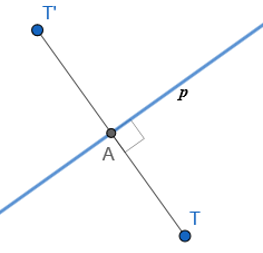
\includegraphics[scale=0.5]{Slike in skice/Zrcaljenje_tocke_cez_premico.png}
                %     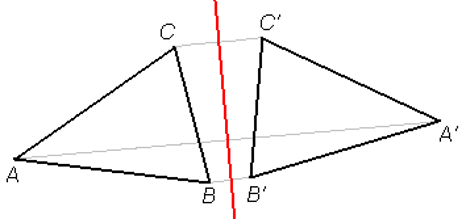
\includegraphics[scale=0.5]{Slike in skice/Zrcaljenje_lika_cez_premico.png}
                % \end{figure}

                \begin{figure}[H]
                    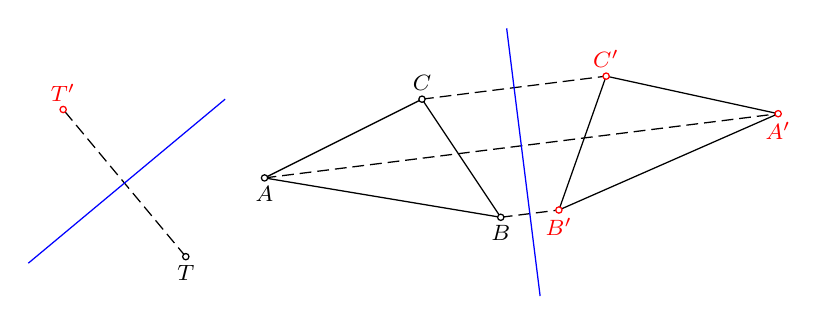
\begin{tikzpicture}
                        % \clip (0,0) rectangle (14.000000,10.000000);
                        {\footnotesize
                        
                        % Marking point T by circle
                        \draw [line width=0.016cm] (3.500000,1.500000) circle (0.040000);%
                        \draw (3.500000,1.500000) node [anchor=north] { $T$ };%
                        
                        % Drawing segment T T'
                        \draw [line width=0.016cm] (3.474393,1.530729) -- (3.403972,1.615233);%
                        \draw [line width=0.016cm] (3.355959,1.672850) -- (3.259931,1.788083);%
                        \draw [line width=0.016cm] (3.211917,1.845700) -- (3.115889,1.960933);%
                        \draw [line width=0.016cm] (3.067876,2.018549) -- (2.971848,2.133783);%
                        \draw [line width=0.016cm] (2.923834,2.191399) -- (2.827806,2.306632);%
                        \draw [line width=0.016cm] (2.779793,2.364249) -- (2.683765,2.479482);%
                        \draw [line width=0.016cm] (2.635751,2.537099) -- (2.539723,2.652332);%
                        \draw [line width=0.016cm] (2.491710,2.709949) -- (2.395682,2.825182);%
                        \draw [line width=0.016cm] (2.347668,2.882798) -- (2.251640,2.998031);%
                        \draw [line width=0.016cm] (2.203627,3.055648) -- (2.107599,3.170881);%
                        \draw [line width=0.016cm] (2.059585,3.228498) -- (1.968230,3.338124);%
                        
                        % Drawing segment C C'
                        \draw [line width=0.016cm] (6.539691,3.504961) -- (6.648842,3.518605);%
                        \draw [line width=0.016cm] (6.723263,3.527908) -- (6.872104,3.546513);%
                        \draw [line width=0.016cm] (6.946525,3.555816) -- (7.095367,3.574421);%
                        \draw [line width=0.016cm] (7.169788,3.583723) -- (7.318629,3.602329);%
                        \draw [line width=0.016cm] (7.393050,3.611631) -- (7.541892,3.630236);%
                        \draw [line width=0.016cm] (7.616313,3.639539) -- (7.765154,3.658144);%
                        \draw [line width=0.016cm] (7.839575,3.667447) -- (7.988417,3.686052);%
                        \draw [line width=0.016cm] (8.062838,3.695355) -- (8.211679,3.713960);%
                        \draw [line width=0.016cm] (8.286100,3.723263) -- (8.434942,3.741868);%
                        \draw [line width=0.016cm] (8.509363,3.751170) -- (8.658204,3.769776);%
                        \draw [line width=0.016cm] (8.732625,3.779078) -- (8.798770,3.787346);%
                        
                        % Drawing segment B B'
                        \draw [line width=0.016cm] (7.539691,2.004961) -- (7.648842,2.018605);%
                        \draw [line width=0.016cm] (7.723263,2.027908) -- (7.872104,2.046513);%
                        \draw [line width=0.016cm] (7.946525,2.055816) -- (8.095367,2.074421);%
                        \draw [line width=0.016cm] (8.169788,2.083723) -- (8.198770,2.087346);%
                        
                        % Drawing segment A A'
                        \draw [line width=0.016cm] (4.539691,2.504961) -- (4.648842,2.518605);%
                        \draw [line width=0.016cm] (4.723263,2.527908) -- (4.872104,2.546513);%
                        \draw [line width=0.016cm] (4.946525,2.555816) -- (5.095367,2.574421);%
                        \draw [line width=0.016cm] (5.169788,2.583723) -- (5.318629,2.602329);%
                        \draw [line width=0.016cm] (5.393050,2.611631) -- (5.541892,2.630236);%
                        \draw [line width=0.016cm] (5.616313,2.639539) -- (5.765154,2.658144);%
                        \draw [line width=0.016cm] (5.839575,2.667447) -- (5.988417,2.686052);%
                        \draw [line width=0.016cm] (6.062838,2.695355) -- (6.211679,2.713960);%
                        \draw [line width=0.016cm] (6.286100,2.723263) -- (6.434942,2.741868);%
                        \draw [line width=0.016cm] (6.509363,2.751170) -- (6.658204,2.769776);%
                        \draw [line width=0.016cm] (6.732625,2.779078) -- (6.881467,2.797683);%
                        \draw [line width=0.016cm] (6.955888,2.806986) -- (7.104729,2.825591);%
                        \draw [line width=0.016cm] (7.179150,2.834894) -- (7.327992,2.853499);%
                        \draw [line width=0.016cm] (7.402413,2.862802) -- (7.551254,2.881407);%
                        \draw [line width=0.016cm] (7.625675,2.890709) -- (7.774517,2.909315);%
                        \draw [line width=0.016cm] (7.848938,2.918617) -- (7.997780,2.937222);%
                        \draw [line width=0.016cm] (8.072200,2.946525) -- (8.221042,2.965130);%
                        \draw [line width=0.016cm] (8.295463,2.974433) -- (8.444305,2.993038);%
                        \draw [line width=0.016cm] (8.518725,3.002341) -- (8.667567,3.020946);%
                        \draw [line width=0.016cm] (8.741988,3.030248) -- (8.890830,3.048854);%
                        \draw [line width=0.016cm] (8.965250,3.058156) -- (9.114092,3.076762);%
                        \draw [line width=0.016cm] (9.188513,3.086064) -- (9.337355,3.104669);%
                        \draw [line width=0.016cm] (9.411775,3.113972) -- (9.560617,3.132577);%
                        \draw [line width=0.016cm] (9.635038,3.141880) -- (9.783880,3.160485);%
                        \draw [line width=0.016cm] (9.858301,3.169788) -- (10.007142,3.188393);%
                        \draw [line width=0.016cm] (10.081563,3.197695) -- (10.230405,3.216301);%
                        \draw [line width=0.016cm] (10.304826,3.225603) -- (10.453667,3.244208);%
                        \draw [line width=0.016cm] (10.528088,3.253511) -- (10.676930,3.272116);%
                        \draw [line width=0.016cm] (10.751351,3.281419) -- (10.900192,3.300024);%
                        \draw [line width=0.016cm] (10.974613,3.309327) -- (10.983386,3.310423);%
                        
                        % Marking point C by circle
                        \draw [line width=0.016cm] (6.500000,3.500000) circle (0.040000);%
                        \draw (6.500000,3.500000) node [anchor=south] { $C$ };%
                        
                        % Marking point A by circle
                        \draw [line width=0.016cm] (4.500000,2.500000) circle (0.040000);%
                        \draw (4.500000,2.500000) node [anchor=north] { $A$ };%
                        
                        % Marking point B by circle
                        \draw [line width=0.016cm] (7.500000,2.000000) circle (0.040000);%
                        \draw (7.500000,2.000000) node [anchor=north] { $B$ };%
                        
                        % Drawing segment A B
                        \draw [line width=0.016cm] (4.539456,2.493424) -- (7.460544,2.006576);%
                        
                        % Drawing segment B C
                        \draw [line width=0.016cm] (7.477812,2.033282) -- (6.522188,3.466718);%
                        
                        % Drawing segment C A
                        \draw [line width=0.016cm] (6.464223,3.482111) -- (4.535777,2.517889);%
                        
                        % Drawing segment C' A'
                        \draw [line width=0.016cm] (8.877541,3.783776) -- (10.983997,3.323916);%
                        
                        % Drawing segment B' C'
                        \draw [line width=0.016cm] (8.251774,2.130027) -- (8.825149,3.754588);%
                        
                        % Drawing segment A' B'
                        \draw [line width=0.016cm] (10.986454,3.299299) -- (8.275085,2.108394);%
                        
                        % Changing color 0 0 255
                        \definecolor{r0g0b255}{rgb}{0.000000,0.000000,1.000000}%
                        \color{r0g0b255}% 
                        
                        % Drawing segment X Y
                        \draw [line width=0.016cm] (4.000000,3.500000) -- (1.500000,1.416667);%
                        
                        % Drawing line r
                        \draw [line width=0.016cm] (8.000000,1.000000) -- (7.575000,4.400000);%
                        
                        % Changing color 255 0 0
                        \definecolor{r255g0b0}{rgb}{1.000000,0.000000,0.000000}%
                        \color{r255g0b0}% 
                        
                        % Marking point T' by circle
                        \draw [line width=0.016cm] (1.942623,3.368852) circle (0.040000);%
                        \draw (1.942623,3.368852) node [anchor=south] { $T'$ };%
                        
                        % Marking point C' by circle
                        \draw [line width=0.016cm] (8.838462,3.792308) circle (0.040000);%
                        \draw (8.838462,3.792308) node [anchor=south] { $C'$ };%
                        
                        % Marking point B' by circle
                        \draw [line width=0.016cm] (8.238462,2.092308) circle (0.040000);%
                        \draw (8.238462,2.092308) node [anchor=north] { $B'$ };%
                        
                        % Marking point A' by circle
                        \draw [line width=0.016cm] (11.023077,3.315385) circle (0.040000);%
                        \draw (11.023077,3.315385) node [anchor=north] { $A'$ };%
                        \color{black}
                        }
                    \end{tikzpicture}
                        
                \end{figure}
            \end{block}
            \begin{block}{}
                Zrcaljenje čez premico daljice preslika v enako dolge daljice, ohranja velikost kotov, ne ohranja orientacije likov, like preslika v skladne like, premic ne preslika v vzporedne premice.
            \end{block}

            % \note{
            %     TABLA: konstrukcija zracljenja točke, daljice in trikotnika preko premice
            %     \\
            %     S pomočjo skic na tabli/okviru ugotavljanje lastnosti zrcaljenja preko premice.
            %     \\
            %     TABLA: Primer enakokrakega trikotnika (osnovnica AC) s simetralo kota z vrhom v C, ki seka c v N. (Dokaz skladnosti trikotnikov ANC in BNC.)
            % }
        \end{frame}

        
        \begin{frame}

            \begin{block}{}
                \textbf{Zrcaljenje čez točko} $O$ preslika točko $T$ v tako točko $T'$, da je $O$ razpolovišče daljice $TT'$. Ta preslikava je enaka vrtenju okrog točke za $180^\circ$.

                % \begin{figure}
                %     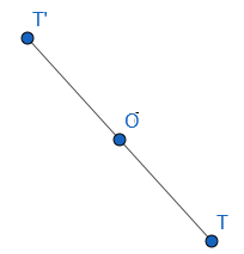
\includegraphics[scale=0.5]{Slike in skice/Zrcaljenje_tocke_cez_tocko.png}
                %     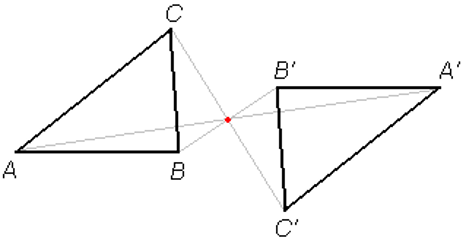
\includegraphics[scale=0.5]{Slike in skice/Zrcaljenje_lika_cez_tocko.png}
                % \end{figure}

                \begin{figure}[H]
                    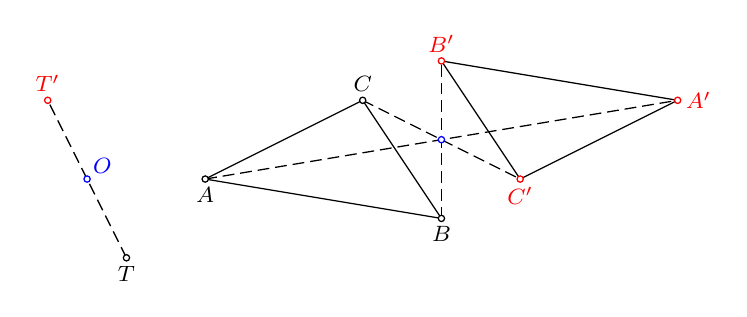
\begin{tikzpicture}
                        % \clip (0,0) rectangle (14.000000,10.000000);
                        {\footnotesize
                        
                        % Marking point T by circle
                        \draw [line width=0.016cm] (3.500000,1.500000) circle (0.040000);%
                        \draw (3.500000,1.500000) node [anchor=north] { $T$ };%
                        
                        % Drawing segment T T'
                        \draw [line width=0.016cm] (3.482111,1.535777) -- (3.432918,1.634164);%
                        \draw [line width=0.016cm] (3.399377,1.701246) -- (3.332295,1.835410);%
                        \draw [line width=0.016cm] (3.298754,1.902492) -- (3.231672,2.036656);%
                        \draw [line width=0.016cm] (3.198131,2.103738) -- (3.131049,2.237902);%
                        \draw [line width=0.016cm] (3.097508,2.304984) -- (3.030426,2.439149);%
                        \draw [line width=0.016cm] (2.982111,2.535777) -- (2.929803,2.640395);%
                        \draw [line width=0.016cm] (2.896262,2.707477) -- (2.829180,2.841641);%
                        \draw [line width=0.016cm] (2.795639,2.908723) -- (2.728557,3.042887);%
                        \draw [line width=0.016cm] (2.695016,3.109969) -- (2.627933,3.244133);%
                        \draw [line width=0.016cm] (2.594392,3.311215) -- (2.527310,3.445379);%
                        
                        % Drawing segment C C'
                        \draw [line width=0.016cm] (6.535777,3.482111) -- (6.634164,3.432918);%
                        \draw [line width=0.016cm] (6.701246,3.399377) -- (6.835410,3.332295);%
                        \draw [line width=0.016cm] (6.902492,3.298754) -- (7.036656,3.231672);%
                        \draw [line width=0.016cm] (7.103738,3.198131) -- (7.237902,3.131049);%
                        \draw [line width=0.016cm] (7.304984,3.097508) -- (7.439149,3.030426);%
                        \draw [line width=0.016cm] (7.535777,2.982111) -- (7.640395,2.929803);%
                        \draw [line width=0.016cm] (7.707477,2.896262) -- (7.841641,2.829180);%
                        \draw [line width=0.016cm] (7.908723,2.795639) -- (8.042887,2.728557);%
                        \draw [line width=0.016cm] (8.109969,2.695016) -- (8.244133,2.627933);%
                        \draw [line width=0.016cm] (8.311215,2.594392) -- (8.445379,2.527310);%
                        
                        % Drawing segment B B'
                        \draw [line width=0.016cm] (7.500000,2.040000) -- (7.500000,2.150000);%
                        \draw [line width=0.016cm] (7.500000,2.225000) -- (7.500000,2.375000);%
                        \draw [line width=0.016cm] (7.500000,2.450000) -- (7.500000,2.600000);%
                        \draw [line width=0.016cm] (7.500000,2.675000) -- (7.500000,2.825000);%
                        \draw [line width=0.016cm] (7.500000,2.900000) -- (7.500000,2.960000);%
                        \draw [line width=0.016cm] (7.500000,3.040000) -- (7.500000,3.050000);%
                        \draw [line width=0.016cm] (7.500000,3.125000) -- (7.500000,3.275000);%
                        \draw [line width=0.016cm] (7.500000,3.350000) -- (7.500000,3.500000);%
                        \draw [line width=0.016cm] (7.500000,3.575000) -- (7.500000,3.725000);%
                        \draw [line width=0.016cm] (7.500000,3.800000) -- (7.500000,3.950000);%
                        
                        % Drawing segment A A'
                        \draw [line width=0.016cm] (4.539456,2.506576) -- (4.647959,2.524660);%
                        \draw [line width=0.016cm] (4.721939,2.536990) -- (4.869898,2.561650);%
                        \draw [line width=0.016cm] (4.943877,2.573980) -- (5.091836,2.598639);%
                        \draw [line width=0.016cm] (5.165816,2.610969) -- (5.313775,2.635629);%
                        \draw [line width=0.016cm] (5.387755,2.647959) -- (5.535714,2.672619);%
                        \draw [line width=0.016cm] (5.609693,2.684949) -- (5.757652,2.709609);%
                        \draw [line width=0.016cm] (5.831632,2.721939) -- (5.979591,2.746598);%
                        \draw [line width=0.016cm] (6.053570,2.758928) -- (6.201530,2.783588);%
                        \draw [line width=0.016cm] (6.275509,2.795918) -- (6.423468,2.820578);%
                        \draw [line width=0.016cm] (6.497448,2.832908) -- (6.645407,2.857568);%
                        \draw [line width=0.016cm] (6.719386,2.869898) -- (6.867345,2.894558);%
                        \draw [line width=0.016cm] (6.941325,2.906887) -- (7.089284,2.931547);%
                        \draw [line width=0.016cm] (7.163264,2.943877) -- (7.311223,2.968537);%
                        \draw [line width=0.016cm] (7.385202,2.980867) -- (7.460544,2.993424);%
                        \draw [line width=0.016cm] (7.607141,3.017857) -- (7.755100,3.042517);%
                        \draw [line width=0.016cm] (7.829079,3.054847) -- (7.977039,3.079506);%
                        \draw [line width=0.016cm] (8.051018,3.091836) -- (8.198977,3.116496);%
                        \draw [line width=0.016cm] (8.272957,3.128826) -- (8.420916,3.153486);%
                        \draw [line width=0.016cm] (8.494895,3.165816) -- (8.642854,3.190476);%
                        \draw [line width=0.016cm] (8.716834,3.202806) -- (8.864793,3.227466);%
                        \draw [line width=0.016cm] (8.938773,3.239795) -- (9.086732,3.264455);%
                        \draw [line width=0.016cm] (9.160711,3.276785) -- (9.308670,3.301445);%
                        \draw [line width=0.016cm] (9.382650,3.313775) -- (9.530609,3.338435);%
                        \draw [line width=0.016cm] (9.604589,3.350765) -- (9.752548,3.375425);%
                        \draw [line width=0.016cm] (9.826527,3.387755) -- (9.974486,3.412414);%
                        \draw [line width=0.016cm] (10.048466,3.424744) -- (10.196425,3.449404);%
                        \draw [line width=0.016cm] (10.270404,3.461734) -- (10.418364,3.486394);%
                        
                        % Marking point C by circle
                        \draw [line width=0.016cm] (6.500000,3.500000) circle (0.040000);%
                        \draw (6.500000,3.500000) node [anchor=south] { $C$ };%
                        
                        % Marking point A by circle
                        \draw [line width=0.016cm] (4.500000,2.500000) circle (0.040000);%
                        \draw (4.500000,2.500000) node [anchor=north] { $A$ };%
                        
                        % Marking point B by circle
                        \draw [line width=0.016cm] (7.500000,2.000000) circle (0.040000);%
                        \draw (7.500000,2.000000) node [anchor=north] { $B$ };%
                        
                        % Drawing segment A B
                        \draw [line width=0.016cm] (4.539456,2.493424) -- (7.460544,2.006576);%
                        
                        % Drawing segment B C
                        \draw [line width=0.016cm] (7.477812,2.033282) -- (6.522188,3.466718);%
                        
                        % Drawing segment C A
                        \draw [line width=0.016cm] (6.464223,3.482111) -- (4.535777,2.517889);%
                        
                        % Drawing segment C' A'
                        \draw [line width=0.016cm] (8.535777,2.517889) -- (10.464223,3.482111);%
                        
                        % Drawing segment B' C'
                        \draw [line width=0.016cm] (7.522188,3.966718) -- (8.477812,2.533282);%
                        
                        % Drawing segment A' B'
                        \draw [line width=0.016cm] (10.460544,3.506576) -- (7.539456,3.993424);%
                        
                        % Changing color 0 0 255
                        \definecolor{r0g0b255}{rgb}{0.000000,0.000000,1.000000}%
                        \color{r0g0b255}% 
                        
                        % Marking point O by circle
                        \draw [line width=0.016cm] (3.000000,2.500000) circle (0.040000);%
                        \draw (2.970000,2.470000) node [anchor=south west] { $O$ };%
                        
                        % Marking point r by circle
                        \draw [line width=0.016cm] (7.500000,3.000000) circle (0.040000);%
                        
                        % Changing color 255 0 0
                        \definecolor{r255g0b0}{rgb}{1.000000,0.000000,0.000000}%
                        \color{r255g0b0}% 
                        
                        % Marking point T' by circle
                        \draw [line width=0.016cm] (2.500000,3.500000) circle (0.040000);%
                        \draw (2.500000,3.500000) node [anchor=south] { $T'$ };%
                        
                        % Marking point C' by circle
                        \draw [line width=0.016cm] (8.500000,2.500000) circle (0.040000);%
                        \draw (8.500000,2.500000) node [anchor=north] { $C'$ };%
                        
                        % Marking point B' by circle
                        \draw [line width=0.016cm] (7.500000,4.000000) circle (0.040000);%
                        \draw (7.500000,4.000000) node [anchor=south] { $B'$ };%
                        
                        % Marking point A' by circle
                        \draw [line width=0.016cm] (10.500000,3.500000) circle (0.040000);%
                        \draw (10.500000,3.500000) node [anchor=west] { $A'$ };%
                        \color{black}
                        }
                    \end{tikzpicture}
                        
                \end{figure}
            \end{block}

            \begin{block}{}
                Zrcaljenje čez točko daljice preslika v enako dolge daljice, ohranja velikosti kotov in orientacijo likov, like preslika v skladne like, premice preslika v vzporedne premice.
            \end{block}

            % \note{
            %     TABLA: konstrukcija zracljenja točke in trikotnika preko točke
            %     \\
            %     S pomočjo skic na tabli/okviru ugotavljanje lastnosti zrcaljenja preko točke.
            % }
        \end{frame}



        \begin{frame}

            \begin{block}{}
                \textbf{Vrtenje} ali \textbf{zasuk} oziroma \textbf{rotacija} za kot $\varphi$ okrog točke $O$ preslika točko $T$ v točko $T'$, da velja: $\left\lvert OT\right\rvert = \left\lvert OT'\right\rvert$  in $\angle TOT' = \varphi$.

                % \begin{figure}
                %     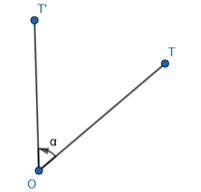
\includegraphics[scale=0.6]{Slike in skice/Rotacija tocke_okoli_tocke.png}
                %     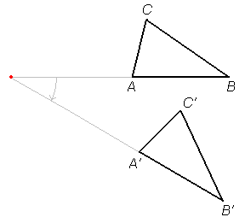
\includegraphics[scale=0.6]{Slike in skice/Rotacija_lika_okoli_tocke.png}
                % \end{figure}

                \begin{figure}[H]
                    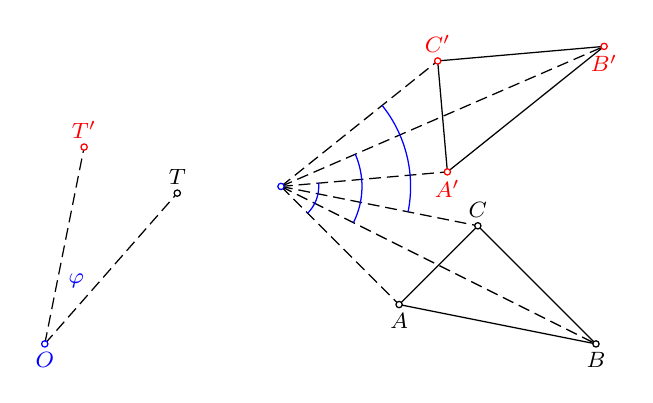
\begin{tikzpicture}
                        % \clip (0,0) rectangle (14.000000,10.000000);
                        {\footnotesize
                        
                        % Drawing segment O T
                        \draw [line width=0.016cm] (1.526405,1.530046) -- (1.599020,1.612672);%
                        \draw [line width=0.016cm] (1.648530,1.669009) -- (1.747550,1.781681);%
                        \draw [line width=0.016cm] (1.797059,1.838017) -- (1.896079,1.950690);%
                        \draw [line width=0.016cm] (1.945589,2.007026) -- (2.044609,2.119698);%
                        \draw [line width=0.016cm] (2.094119,2.176035) -- (2.193139,2.288707);%
                        \draw [line width=0.016cm] (2.242649,2.345043) -- (2.341668,2.457716);%
                        \draw [line width=0.016cm] (2.391178,2.514052) -- (2.490198,2.626724);%
                        \draw [line width=0.016cm] (2.539708,2.683060) -- (2.638728,2.795733);%
                        \draw [line width=0.016cm] (2.688238,2.852069) -- (2.787258,2.964742);%
                        \draw [line width=0.016cm] (2.836768,3.021078) -- (2.935787,3.133750);%
                        \draw [line width=0.016cm] (2.985297,3.190086) -- (3.084317,3.302759);%
                        \draw [line width=0.016cm] (3.133827,3.359095) -- (3.156608,3.385017);%
                        
                        % Drawing segment O T'
                        \draw [line width=0.016cm] (1.507845,1.539223) -- (1.529417,1.647087);%
                        \draw [line width=0.016cm] (1.544126,1.720631) -- (1.573544,1.867718);%
                        \draw [line width=0.016cm] (1.588252,1.941261) -- (1.617670,2.088348);%
                        \draw [line width=0.016cm] (1.632378,2.161892) -- (1.661796,2.308979);%
                        \draw [line width=0.016cm] (1.676505,2.382523) -- (1.705922,2.529610);%
                        \draw [line width=0.016cm] (1.720631,2.603153) -- (1.750048,2.750240);%
                        \draw [line width=0.016cm] (1.764757,2.823784) -- (1.794174,2.970871);%
                        \draw [line width=0.016cm] (1.808883,3.044415) -- (1.838300,3.191502);%
                        \draw [line width=0.016cm] (1.853009,3.265045) -- (1.882426,3.412132);%
                        \draw [line width=0.016cm] (1.897135,3.485676) -- (1.926553,3.632763);%
                        \draw [line width=0.016cm] (1.941261,3.706307) -- (1.970679,3.853394);%
                        \draw [line width=0.016cm] (1.985387,3.926937) -- (1.992155,3.960777);%
                        
                        % Marking point C by circle
                        \draw [line width=0.016cm] (7.000000,3.000000) circle (0.040000);%
                        \draw (7.000000,3.000000) node [anchor=south] { $C$ };%
                        
                        % Marking point A by circle
                        \draw [line width=0.016cm] (6.000000,2.000000) circle (0.040000);%
                        \draw (6.000000,2.000000) node [anchor=north] { $A$ };%
                        
                        % Marking point B by circle
                        \draw [line width=0.016cm] (8.500000,1.500000) circle (0.040000);%
                        \draw (8.500000,1.500000) node [anchor=north] { $B$ };%
                        
                        % Drawing segment A B
                        \draw [line width=0.016cm] (6.039223,1.992155) -- (8.460777,1.507845);%
                        
                        % Drawing segment B C
                        \draw [line width=0.016cm] (8.471716,1.528284) -- (7.028284,2.971716);%
                        
                        % Drawing segment A C
                        \draw [line width=0.016cm] (6.028284,2.028284) -- (6.971716,2.971716);%
                        
                        % Drawing segment X A
                        \draw [line width=0.016cm] (4.528284,3.471716) -- (4.606066,3.393934);%
                        \draw [line width=0.016cm] (4.659099,3.340901) -- (4.765165,3.234835);%
                        \draw [line width=0.016cm] (4.818198,3.181802) -- (4.924264,3.075736);%
                        \draw [line width=0.016cm] (4.977297,3.022703) -- (5.083363,2.916637);%
                        \draw [line width=0.016cm] (5.136396,2.863604) -- (5.242462,2.757538);%
                        \draw [line width=0.016cm] (5.295495,2.704505) -- (5.401561,2.598439);%
                        \draw [line width=0.016cm] (5.454594,2.545406) -- (5.560660,2.439340);%
                        \draw [line width=0.016cm] (5.613693,2.386307) -- (5.719759,2.280241);%
                        \draw [line width=0.016cm] (5.772792,2.227208) -- (5.878858,2.121142);%
                        \draw [line width=0.016cm] (5.931891,2.068109) -- (5.971716,2.028284);%
                        
                        % Drawing segment X B
                        \draw [line width=0.016cm] (4.535777,3.482111) -- (4.634164,3.432918);%
                        \draw [line width=0.016cm] (4.701246,3.399377) -- (4.835410,3.332295);%
                        \draw [line width=0.016cm] (4.902492,3.298754) -- (5.036656,3.231672);%
                        \draw [line width=0.016cm] (5.103738,3.198131) -- (5.237902,3.131049);%
                        \draw [line width=0.016cm] (5.304984,3.097508) -- (5.439149,3.030426);%
                        \draw [line width=0.016cm] (5.506231,2.996885) -- (5.640395,2.929803);%
                        \draw [line width=0.016cm] (5.707477,2.896262) -- (5.841641,2.829180);%
                        \draw [line width=0.016cm] (5.908723,2.795639) -- (6.042887,2.728557);%
                        \draw [line width=0.016cm] (6.109969,2.695016) -- (6.244133,2.627933);%
                        \draw [line width=0.016cm] (6.311215,2.594392) -- (6.445379,2.527310);%
                        \draw [line width=0.016cm] (6.512461,2.493769) -- (6.646625,2.426687);%
                        \draw [line width=0.016cm] (6.713707,2.393146) -- (6.847871,2.326064);%
                        \draw [line width=0.016cm] (6.914953,2.292523) -- (7.049117,2.225441);%
                        \draw [line width=0.016cm] (7.116200,2.191900) -- (7.250364,2.124818);%
                        \draw [line width=0.016cm] (7.317446,2.091277) -- (7.451610,2.024195);%
                        \draw [line width=0.016cm] (7.518692,1.990654) -- (7.652856,1.923572);%
                        \draw [line width=0.016cm] (7.719938,1.890031) -- (7.854102,1.822949);%
                        \draw [line width=0.016cm] (7.921184,1.789408) -- (8.055348,1.722326);%
                        \draw [line width=0.016cm] (8.122430,1.688785) -- (8.256594,1.621703);%
                        \draw [line width=0.016cm] (8.323676,1.588162) -- (8.457840,1.521080);%
                        
                        % Drawing segment X C
                        \draw [line width=0.016cm] (4.539223,3.492155) -- (4.647087,3.470583);%
                        \draw [line width=0.016cm] (4.720631,3.455874) -- (4.867718,3.426456);%
                        \draw [line width=0.016cm] (4.941261,3.411748) -- (5.088348,3.382330);%
                        \draw [line width=0.016cm] (5.161892,3.367622) -- (5.308979,3.338204);%
                        \draw [line width=0.016cm] (5.382523,3.323495) -- (5.529610,3.294078);%
                        \draw [line width=0.016cm] (5.603153,3.279369) -- (5.750240,3.249952);%
                        \draw [line width=0.016cm] (5.823784,3.235243) -- (5.970871,3.205826);%
                        \draw [line width=0.016cm] (6.044415,3.191117) -- (6.191502,3.161700);%
                        \draw [line width=0.016cm] (6.265045,3.146991) -- (6.412132,3.117574);%
                        \draw [line width=0.016cm] (6.485676,3.102865) -- (6.632763,3.073447);%
                        \draw [line width=0.016cm] (6.706307,3.058739) -- (6.853394,3.029321);%
                        \draw [line width=0.016cm] (6.926937,3.014613) -- (6.960777,3.007845);%
                        
                        % Drawing segment A' B'
                        \draw [line width=0.016cm] (6.644470,3.709889) -- (8.572018,5.253598);%
                        
                        % Drawing segment B' C'
                        \draw [line width=0.016cm] (8.563392,5.275116) -- (6.529839,5.097203);%
                        
                        % Drawing segment A' C'
                        \draw [line width=0.016cm] (6.609762,3.724733) -- (6.493478,5.053869);%
                        
                        % Drawing segment X A'
                        \draw [line width=0.016cm] (4.539848,3.503486) -- (4.649429,3.513073);%
                        \draw [line width=0.016cm] (4.724144,3.519610) -- (4.873573,3.532683);%
                        \draw [line width=0.016cm] (4.948288,3.539220) -- (5.097717,3.552293);%
                        \draw [line width=0.016cm] (5.172431,3.558830) -- (5.321861,3.571903);%
                        \draw [line width=0.016cm] (5.396575,3.578440) -- (5.546004,3.591513);%
                        \draw [line width=0.016cm] (5.620719,3.598050) -- (5.770148,3.611124);%
                        \draw [line width=0.016cm] (5.844863,3.617660) -- (5.994292,3.630734);%
                        \draw [line width=0.016cm] (6.069007,3.637270) -- (6.218436,3.650344);%
                        \draw [line width=0.016cm] (6.293150,3.656880) -- (6.442580,3.669954);%
                        \draw [line width=0.016cm] (6.517294,3.676490) -- (6.573400,3.681399);%
                        
                        % Drawing segment X B'
                        \draw [line width=0.016cm] (4.536700,3.515908) -- (4.637627,3.559656);%
                        \draw [line width=0.016cm] (4.706440,3.589484) -- (4.844067,3.649140);%
                        \draw [line width=0.016cm] (4.912881,3.678968) -- (5.050507,3.738625);%
                        \draw [line width=0.016cm] (5.119321,3.768453) -- (5.256948,3.828109);%
                        \draw [line width=0.016cm] (5.325761,3.857937) -- (5.463388,3.917593);%
                        \draw [line width=0.016cm] (5.532201,3.947421) -- (5.669828,4.007077);%
                        \draw [line width=0.016cm] (5.738642,4.036905) -- (5.876268,4.096561);%
                        \draw [line width=0.016cm] (5.945082,4.126389) -- (6.082709,4.186046);%
                        \draw [line width=0.016cm] (6.151522,4.215874) -- (6.289149,4.275530);%
                        \draw [line width=0.016cm] (6.357962,4.305358) -- (6.495589,4.365014);%
                        \draw [line width=0.016cm] (6.564403,4.394842) -- (6.702029,4.454498);%
                        \draw [line width=0.016cm] (6.770843,4.484326) -- (6.908470,4.543982);%
                        \draw [line width=0.016cm] (6.977283,4.573810) -- (7.114910,4.633467);%
                        \draw [line width=0.016cm] (7.183723,4.663295) -- (7.321350,4.722951);%
                        \draw [line width=0.016cm] (7.390164,4.752779) -- (7.527790,4.812435);%
                        \draw [line width=0.016cm] (7.596604,4.842263) -- (7.734231,4.901919);%
                        \draw [line width=0.016cm] (7.803044,4.931747) -- (7.940671,4.991403);%
                        \draw [line width=0.016cm] (8.009484,5.021232) -- (8.147111,5.080888);%
                        \draw [line width=0.016cm] (8.215925,5.110716) -- (8.353551,5.170372);%
                        \draw [line width=0.016cm] (8.422365,5.200200) -- (8.559992,5.259856);%
                        
                        % Drawing segment X C'
                        \draw [line width=0.016cm] (4.531222,3.525004) -- (4.617081,3.593766);%
                        \draw [line width=0.016cm] (4.675621,3.640649) -- (4.792702,3.734415);%
                        \draw [line width=0.016cm] (4.851242,3.781298) -- (4.968323,3.875064);%
                        \draw [line width=0.016cm] (5.026864,3.921947) -- (5.143945,4.015714);%
                        \draw [line width=0.016cm] (5.202485,4.062597) -- (5.319566,4.156363);%
                        \draw [line width=0.016cm] (5.378106,4.203246) -- (5.495187,4.297012);%
                        \draw [line width=0.016cm] (5.553727,4.343895) -- (5.670808,4.437661);%
                        \draw [line width=0.016cm] (5.729349,4.484544) -- (5.846429,4.578310);%
                        \draw [line width=0.016cm] (5.904970,4.625193) -- (6.022051,4.718959);%
                        \draw [line width=0.016cm] (6.080591,4.765842) -- (6.197672,4.859608);%
                        \draw [line width=0.016cm] (6.256212,4.906491) -- (6.373293,5.000258);%
                        \draw [line width=0.016cm] (6.431834,5.047141) -- (6.458770,5.068713);%
                        
                        % Marking point T by circle
                        \draw [line width=0.016cm] (3.183013,3.415063) circle (0.040000);%
                        \draw (3.183013,3.415063) node [anchor=south] { $T$ };%
                        
                        % Changing color 0 0 255
                        \definecolor{r0g0b255}{rgb}{0.000000,0.000000,1.000000}%
                        \color{r0g0b255}% 
                        
                        % Marking point O by circle
                        \draw [line width=0.016cm] (1.500000,1.500000) circle (0.040000);%
                        \draw (1.500000,1.500000) node [anchor=north] { $O$ };%
                        
                        % Marking point \alpha
                        \draw (1.900000,2.300000) node  { $\varphi$ };%
                        
                        % Marking point X by circle
                        \draw [line width=0.016cm] (4.500000,3.500000) circle (0.040000);%
                        
                        % Drawing arc X a 50.00
                        \draw [line width=0.016cm] (4.839000,3.161000) -- (4.839000,3.161000) arc (315:360:0.479418 and 0.479418) --(4.979418,3.500000) arc (0:4:0.479418 and 0.479418) -- (4.977594,3.541784);%
                        
                        % Drawing arc X b 50.00
                        \draw [line width=0.016cm] (5.420000,3.040000) -- (5.424492,3.049095) arc (334:360:1.028591 and 1.028591) --(5.528591,3.500000) arc (0:23:1.028591 and 1.028591) -- (5.443745,3.909079);%
                        
                        % Drawing arc X c 50.00
                        \draw [line width=0.016cm] (6.114000,3.177000) -- (6.115761,3.185927) arc (349:360:1.646003 and 1.646003) --(6.146003,3.500000) arc (0:38:1.646003 and 1.646003) -- (5.784892,4.528775);%
                        
                        % Changing color 255 0 0
                        \definecolor{r255g0b0}{rgb}{1.000000,0.000000,0.000000}%
                        \color{r255g0b0}% 
                        
                        % Marking point T' by circle
                        \draw [line width=0.016cm] (2.000000,4.000000) circle (0.040000);%
                        \draw (2.000000,4.000000) node [anchor=south] { $T'$ };%
                        
                        % Marking point A' by circle
                        \draw [line width=0.016cm] (6.613248,3.684885) circle (0.040000);%
                        \draw (6.613248,3.684885) node [anchor=north] { $A'$ };%
                        
                        % Marking point B' by circle
                        \draw [line width=0.016cm] (8.603239,5.278602) circle (0.040000);%
                        \draw (8.603239,5.278602) node [anchor=north] { $B'$ };%
                        
                        % Marking point C' by circle
                        \draw [line width=0.016cm] (6.489991,5.093717) circle (0.040000);%
                        \draw (6.489991,5.093717) node [anchor=south] { $C'$ };%
                        \color{black}
                        }
                    \end{tikzpicture}
                \end{figure}
            \end{block}

            \begin{block}{}
                Vrtenje okoli točke preslika daljice v enako dolge daljice, ohranja velikosti kotov in orientacijo likov, like preslika v skladne like, premic pa ne preslika v vzporedne premice.
            \end{block}

            % \note{
            %     TABLA: konstrukcija rotacije točke okoli točke za nek kot; rotacija trikotnika za isti kot
            %     \\
            %     Opomba: vrtenje v pozitivni/negativni smeri oziroma za pozitiven/negativen kot
            %     \\
            %     S pomočjo skic na tabli/okviru ugotovitev lastnosti dane prelikave.

            % }
        \end{frame}



        \begin{frame}
            \frametitle{Simetrija}

            \begin{columns}
                \column{0.65\textwidth}
                ~\\
                Množica točk $\mathcal{M}$ je \textbf{simetrična/somerna glede na premico} $p$, 
                če se pri zrcaljenju čez premico $p$ preslika sama vase. 
                Premico $p$ imenujemo \textbf{simetrala}/\textbf{somernica}/\textbf{simetrijska os} množice $\mathcal{M}$. 
                 ~\\      
                 ~\\      
                Množica točk $\mathcal{M}$ je \textbf{središčno simetrična/somerna glede na točko} $T$, 
                če se pri zrcaljenju čez točko $T$ preslika sama vase. 
                Točko $T$ imenujemo \textbf{center simetrije} množice $\mathcal{M}$. 
                \column{0.32\textwidth}
                \begin{figure}
                    % 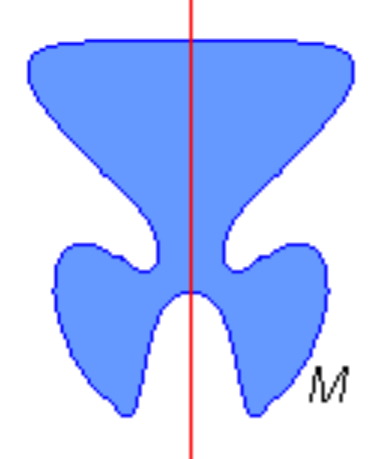
\includegraphics[scale=0.25]{../Slike in skice/Simetrija glede na premico.png}

                    % 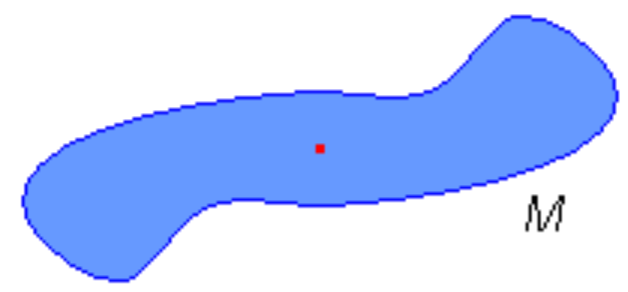
\includegraphics[scale=0.25]{../Slike in skice/Simetrija glede na točko.png}
                \end{figure}
            \end{columns}


            % \note{
            %     Ponovitev definicije in konstrukcije simetrale daljice in simetrale kota.
            % }
        \end{frame}




        

        %%%%%%%% naloge

        \begin{frame}
            \only<2->{\begin{exampleblock}{Naloga}
                Narišite kvadrat s stranico dolžine $1$ in ga:
                \begin{itemize}
                    \item vzporedno premaknite vzdolž ordinatne osi za $3$ enota;
                    \item zavrtite okrog oglišča $B$ za kot $45^\circ$ v negativni smeri;
                    \item zrcalite preko nosilke stranice $CD$.
                \end{itemize}
            \end{exampleblock}}

            \only<3->{\begin{exampleblock}{Naloga}
                Izračunajte velikosti kotov $\alpha$, $\beta$ in $\gamma$. Podatke razberite iz skic. Velja $p\parallel q$ in $r\parallel s$.
                \begin{figure}
                    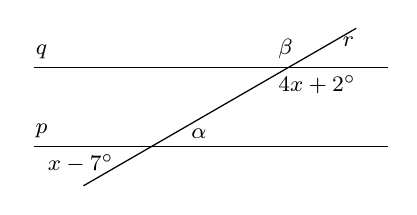
\begin{tikzpicture}
                        % \clip (0,0) rectangle (14.000000,10.000000);
                        {\footnotesize

                        % Drawing line Q
                        \draw [line width=0.016cm] (1.500000,1.500000) -- (6.000000,1.500000);%

                        % Drawing line P
                        \draw [line width=0.016cm] (1.500000,2.500000) -- (6.000000,2.500000);%

                        % Drawing line R
                        \draw [line width=0.016cm] (2.133975,1.000000) -- (5.598076,3.000000);%

                        % Marking point p
                        \draw (1.600000,1.500000) node [anchor=south] { $p$ };%

                        % Marking point q
                        \draw (1.600000,2.500000) node [anchor=south] { $q$ };%

                        % Marking point r
                        \draw (5.500000,3.000000) node [anchor=north] { $r$ };%

                        % Marking point \alpha
                        \draw (3.600000,1.500000) node [anchor=south] { $\alpha$ };%

                        % Marking point \beta
                        \draw (4.700000,2.500000) node [anchor=south] { $\beta$ };%

                        % Marking point {4x+2^\circ}
                        \draw (5.100000,2.500000) node [anchor=north] { ${4x+2^\circ}$ };%

                        % Marking point {x-7^\circ}
                        \draw (2.100000,1.500000) node [anchor=north] { ${x-7^\circ}$ };%
                        }
                    \end{tikzpicture} ~
                    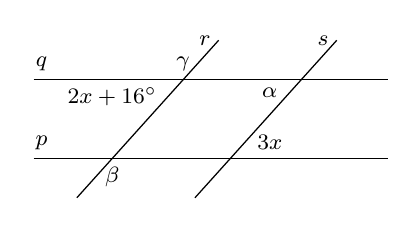
\begin{tikzpicture}
                        % \clip (0,0) rectangle (14.000000,10.000000);
                        {\footnotesize

                        % Drawing line Q
                        \draw [line width=0.016cm] (1.500000,1.500000) -- (6.000000,1.500000);%

                        % Drawing line P
                        \draw [line width=0.016cm] (1.500000,2.500000) -- (6.000000,2.500000);%

                        % Drawing line R
                        \draw [line width=0.016cm] (2.049798,1.000000) -- (3.850606,3.000000);%

                        % Drawing line S
                        \draw [line width=0.016cm] (3.549798,1.000000) -- (5.350606,3.000000);%

                        % Marking point p
                        \draw (1.600000,1.500000) node [anchor=south] { $p$ };%

                        % Marking point q
                        \draw (1.600000,2.500000) node [anchor=south] { $q$ };%

                        % Marking point r
                        \draw (3.500000,3.000000) node [anchor=west] { $r$ };%

                        % Marking point s
                        \draw (5.000000,3.000000) node [anchor=west] { $s$ };%

                        % Marking point \alpha
                        \draw (4.500000,2.500000) node [anchor=north] { $\alpha$ };%

                        % Marking point \beta
                        \draw (2.500000,1.500000) node [anchor=north] { $\beta$ };%

                        % Marking point \gamma
                        \draw (3.400000,2.500000) node [anchor=south] { $\gamma$ };%

                        % Marking point {3x}
                        \draw (4.500000,1.500000) node [anchor=south] { ${3x}$ };%

                        % Marking point {2x+16^\circ}
                        \draw (2.500000,2.500000) node [anchor=north] { ${2x+16^\circ}$ };%
                        }
                    \end{tikzpicture} ~
                    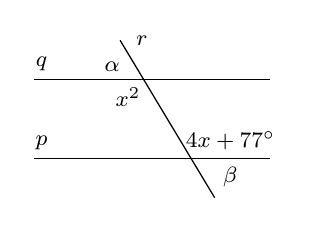
\begin{tikzpicture}
                        % \clip (0,0) rectangle (14.000000,10.000000);
                        {\footnotesize

                        % Drawing line Q
                        \draw [line width=0.016cm] (1.500000,1.500000) -- (4.500000,1.500000);%

                        % Drawing line P
                        \draw [line width=0.016cm] (1.500000,2.500000) -- (4.500000,2.500000);%

                        % Drawing line R
                        \draw [line width=0.016cm] (3.800430,1.000000) -- (2.598709,3.000000);%

                        % Marking point p
                        \draw (1.600000,1.500000) node [anchor=south] { $p$ };%

                        % Marking point q
                        \draw (1.600000,2.500000) node [anchor=south] { $q$ };%

                        % Marking point r
                        \draw (2.700000,3.000000) node [anchor=west] { $r$ };%

                        % Marking point \alpha
                        \draw (2.500000,2.500000) node [anchor=south] { $\alpha$ };%

                        % Marking point \beta
                        \draw (4.000000,1.500000) node [anchor=north] { $\beta$ };%

                        % Marking point {4x+77^\circ}
                        \draw (4.000000,1.500000) node [anchor=south] { ${4x+77^\circ}$ };%

                        % Marking point {x^2}
                        \draw (2.700000,2.500000) node [anchor=north] { ${x^2}$ };%
                        }
                    \end{tikzpicture}
                \end{figure}
            \end{exampleblock}}
        \end{frame}

        \begin{frame}

            \only<2->{\begin{exampleblock}{Naloga}
                S skice preberite ustrezne podatke ter izračunajte velikosti kotov $\alpha$, $\beta$, $\gamma$ in $\delta$.
                Pri tem velja, da so premice $p$, $q$ in $r$ vzporedne.
                \begin{figure}
                    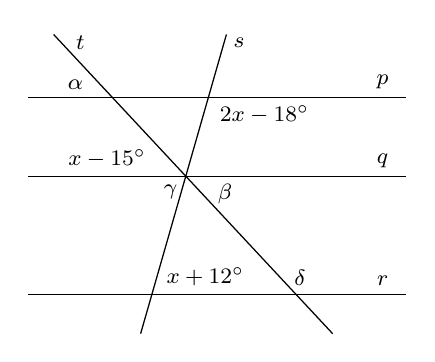
\begin{tikzpicture}
                        % \clip (0,0) rectangle (14.000000,10.000000);
                        {\footnotesize

                        % Drawing line Q
                        \draw [line width=0.016cm] (1.000000,3.000000) -- (5.800000,3.000000);%

                        % Drawing line P
                        \draw [line width=0.016cm] (1.000000,4.000000) -- (5.800000,4.000000);%

                        % Drawing line R
                        \draw [line width=0.016cm] (1.000000,1.500000) -- (5.800000,1.500000);%

                        % Drawing line S
                        \draw [line width=0.016cm] (2.426509,1.000000) -- (3.516142,4.800000);%

                        % Drawing line T
                        \draw [line width=0.016cm] (4.865030,1.000000) -- (1.321473,4.800000);%

                        % Marking point p
                        \draw (5.500000,4.000000) node [anchor=south] { $p$ };%

                        % Marking point q
                        \draw (5.500000,3.000000) node [anchor=south] { $q$ };%

                        % Marking point r
                        \draw (5.500000,1.500000) node [anchor=south] { $r$ };%

                        % Marking point s
                        \draw (3.500000,4.700000) node [anchor=west] { $s$ };%

                        % Marking point t
                        \draw (1.500000,4.700000) node [anchor=west] { $t$ };%

                        % Marking point \alpha
                        \draw (1.800000,4.000000) node [anchor=south east] { $\alpha$ };%

                        % Marking point \beta
                        \draw (3.300000,3.000000) node [anchor=north west] { $\beta$ };%

                        % Marking point \gamma
                        \draw (3.000000,3.000000) node [anchor=north east] { $\gamma$ };%

                        % Marking point \delta
                        \draw (4.450000,1.500000) node [anchor=south] { $\delta$ };%

                        % Marking point {x-15^\circ}
                        \draw (2.000000,3.000000) node [anchor=south] { ${x-15^\circ}$ };%

                        % Marking point {2x-18^\circ}
                        \draw (4.000000,4.000000) node [anchor=north] { ${2x-18^\circ}$ };%

                        % Marking point {x+12^\circ}
                        \draw (3.250000,1.500000) node [anchor=south] { ${x+12^\circ}$ };%
                        }
                    \end{tikzpicture}

                \end{figure}
            \end{exampleblock}}

        \end{frame}





%%%%%%%%%%%%%%%%%%%%%%%%%%%%%%%%

    \subsection{Trikotnik}

        \begin{frame}
            \frametitle{Trikotnik}

            \vskip-1em
            \begin{alertblock}{Definicija}
                \textbf{Trikotnik} je lik/množica točk v ravnini, omejena s tremi daljicami -- \textbf{stranicami} ($a, b, c$), ki povezujejo tri nekolinearne točke ($A, B, C$) v ravnini. Te točke imenujemo \textbf{oglišča} trikotnika.
            
            % \begin{figure}
            %     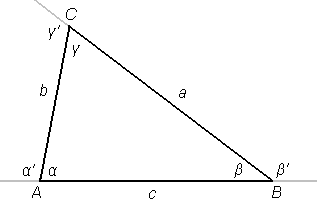
\includegraphics[scale=0.7]{Slike in skice/Trikotnik.png}    
            % \end{figure}

            \begin{figure}
                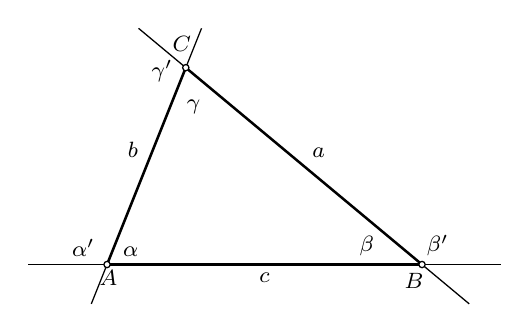
\begin{tikzpicture}
                    % \clip (0,0) rectangle (14.000000,10.000000);
                    {\footnotesize
                    
                    % Marking point A by circle
                    \draw<2-> [line width=0.016cm] (2.000000,1.500000) circle (0.040000);%
                    \draw<2-> (1.800000,1.530000) node [anchor=north west] { $A$ };%
                    
                    % Marking point B by circle
                    \draw<2-> [line width=0.016cm] (6.000000,1.500000) circle (0.040000);%
                    \draw<2-> (5.900000,1.500000) node [anchor=north] { $B$ };%
                    
                    % Marking point C by circle
                    \draw<2-> [line width=0.016cm] (3.000000,4.000000) circle (0.040000);%
                    \draw<2-> (2.950000,4.100000) node [anchor=south] { $C$ };%
                    
                    % Drawing line A B
                    \draw<4-> [line width=0.016cm] (1.000000,1.500000) -- (1.960000,1.500000);%
                    \draw<4-> [line width=0.016cm] (2.040000,1.500000) -- (5.960000,1.500000);%
                    \draw<4-> [line width=0.016cm] (6.040000,1.500000) -- (7.000000,1.500000);%
                    
                    % Drawing line B C
                    \draw<4-> [line width=0.016cm] (6.600000,1.000000) -- (6.030729,1.474393);%
                    \draw<4-> [line width=0.016cm] (5.969271,1.525607) -- (3.030729,3.974393);%
                    \draw<4-> [line width=0.016cm] (2.969271,4.025607) -- (2.400000,4.500000);%
                    
                    % Drawing line A C
                    \draw<4-> [line width=0.016cm] (1.800000,1.000000) -- (1.985144,1.462861);%
                    \draw<4-> [line width=0.016cm] (2.014856,1.537139) -- (2.985144,3.962861);%
                    \draw<4-> [line width=0.016cm] (3.014856,4.037139) -- (3.200000,4.500000);%
                    
                    % Marking point c
                    \draw<2-> (4.000000,1.500000) node [anchor=north] { $c$ };%
                    
                    % Marking point a
                    \draw<2-> (4.500000,2.750000) node [anchor=south west] { $a$ };%
                    
                    % Marking point b
                    \draw<2-> (2.500000,2.750000) node [anchor=south east] { $b$ };%
                    
                    % Marking point \gamma
                    \draw<3-> (3.100000,3.700000) node [anchor=north] { $\gamma$ };%
                    
                    % Marking point \gamma'
                    \draw<4-> (2.700000,4.200000) node [anchor=north] { $\gamma'$ };%
                    
                    % Marking point \beta
                    \draw<3-> (5.300000,1.500000) node [anchor=south] { $\beta$ };%
                    
                    % Marking point \beta'
                    \draw<4-> (6.200000,1.500000) node [anchor=south] { $\beta'$ };%
                    
                    % Marking point \alpha
                    \draw<3-> (2.300000,1.500000) node [anchor=south] { $\alpha$ };%
                    
                    % Marking point \alpha'
                    \draw<4-> (1.700000,1.500000) node [anchor=south] { $\alpha'$ };%
                    
                    % Drawing segment A B
                    \draw<2-> [line width=0.032cm] (2.040000,1.500000) -- (5.960000,1.500000);%
                    
                    % Drawing segment B C
                    \draw<2-> [line width=0.032cm] (5.969271,1.525607) -- (3.030729,3.974393);%
                    
                    % Drawing segment A C
                    \draw<2-> [line width=0.032cm] (2.014856,1.537139) -- (2.985144,3.962861);%
                    }
                \end{tikzpicture}
            \end{figure}

             \end{alertblock}
           

            \begin{block}{}
                V trikotniku $\triangle ABC$  so $\alpha, \beta$ in $\gamma$ \textbf{notranji koti}, njihovi sokoti $\alpha', \beta'$ in $\gamma'$ pa so \textbf{zunanji koti}. 
            \end{block}
            

        \end{frame}


        \begin{frame}
            
            \begin{block}{Izrek}
                Vsota notranjih kotov trikotnika je $180^\circ$: 
                \vskip-1em
                $$\alpha+\beta+\gamma=180^\circ.$$ 
            \end{block}

            
            \begin{block}{Izrek}
                Zunanji kot trikotnika je enak vsoti notranjih nepriležnih kotov: 
                \vskip-1em
                \begin{align*}
                    \alpha' &= \beta+\gamma \\
                    \beta' &= \alpha+\gamma \\
                    \gamma' &= \alpha+\beta
                \end{align*}
            \end{block}

            
            \begin{block}{Izrek}
                Vsota zunanjih kotov trikotnika je $360^\circ$: 
                \vskip-1em
                $$\alpha'+\beta'+\gamma'=360^\circ.$$ 
            \end{block}


            % \note{
            %     DOKAZ 1. izreka: Upoštevamo lastnosti kotov z vzporednimi kraki. Narišemo nosilko stranice $a$ preko oglišča $C$. Konstruiramo vzpordnico k $c$ skozi $C$. Dobljena kota sta skladna $\alpha$ oziroma $\beta$. Vsi trije koti skupaj tvorijo iztegnjeni kot ($180^\circ$).
            %     \\
            %     DOKAZ 2. izreka: Dokaz naredimo zgolj za enega izmed kotov: Na skici dokaz prejšnjega izreka vidimo, da je zunanji kot pri oglišču $C$ enak vsoti kotov $\alpha$ in $\beta$.
            %     \\
            %     DOKAZ 3. izreka: Po prejšnjih dveh izrekih sledi, da je $\alpha'+\beta'+\gamma'=2\cdot(\alpha+\beta+\gamma)=2\cdot180^\circ=360^\circ$.
            % }
        \end{frame}


        % \begin{frame}
        %     \begin{exampleblock}{Naloga 65}
        %         Izračunaj velikosti notranjih in zunanjih kotov trikotnika $\triangle ABC$, če je $\alpha= 67^\circ 13'$ in $\beta' = 133^\circ 25'$.
        %     \end{exampleblock}

        %     \pause
        %     \begin{exampleblock}{Naloga 68}
        %         Velikosti notranjih kotov trikotnika so v razmerju $2:5:11$. V kolikšnem razmerju so velikosti zunanjih kotov tega trikotnika?
        %     \end{exampleblock}

        %     \pause
        %     \begin{exampleblock}{Naloga 70}
        %         Notranji kot ob oglišču $A$ trikotnika $\triangle ABC$ je za $1^\circ$ manjši od velikosti notranjega kota ob oglišču $C$.  Zunanji kot v oglišču $C$ je za $1^\circ$ večji od dvakratnika velikosti notranjega kota ob oglišču $A$. Izračunaj velikosti notranjih kotov trikotnika $\triangle ABC$.
        %     \end{exampleblock}
        % \end{frame}
        

        \begin{frame}
            
            \begin{block}{Izrek}
                Nasproti daljše stranice trikotnika leži večji notranji kot, nasproti krajše stranice pa manjši notranji kot trikotnika.
                \vskip-1em
                $$a>b \Leftrightarrow \alpha > \beta$$
            \end{block}

            
            \begin{block}{Izrek (Trikotniška neenakost)}
                Vsaka stranica trikotnika je krajša od vsote dolžin drugih dveh stranic.
                \vskip-1em
                \begin{align*}
                    a &< b + c \\
                    b &< a + c \\
                    c &< a + b
                \end{align*}
            \end{block}

            
            \begin{block}{Izrek}
                Vsaka stranica trikotnika je daljša od absolutne vrednosti razlike dolžin drugih dveh stranic.
            \end{block}


            \note{
                DOKAZ 1. izreka: Denimo, da je $c$ daljša od $b$ v trikotniku $ABC$. Konstruiramo simetralo $\alpha$ in označimo presečišče z $a$ z $D$. Daljico $AC$ prenesemo na $AB$ in točko označimo z $E$. Dobili smo skladna trikotnika $AED$ in $ACD$ (skupna $AD$, $|AC|=|AE|$, kot med njima). Torej je $\angle DEA = \gamma$ zunanji kot za trikotnik $EBD$, torej enak vsoti $\beta$ in $\angle EDB$. To pomeni da velja $\gamma > \beta$.
                \\
                DOKAZ 2. izreka: Dokaz naredimo zgolj za eno neenakost: Podaljšamo eno izmed stranic trikotnika $ABC$, naj bo to $a$, preko oglišča $C$ za dolžino stranice $b$. Dobili smo enakokrak trikotnik $ACC'$, skladna kota $\angle CAC'$ in $\angle AC'C$ označimo z $\varphi$. Kot $\angle BAC' = \epsilon$ je večji od $\varphi$. V trikotniku $ABC'$ je $\epsilon > \varphi$, zato je $BC' > c$. To nam da: $c<a+b$.
            }
        \end{frame}


        % \begin{frame}
        %     \begin{exampleblock}{Naloga 76}
        %         Ali obstaja trikotnik z danimi dolžinami stranic?
        %         \begin{enumerate}
        %             \item $a=4~cm,\ b=5~cm,\ c=10~cm$;
        %             \item $a=4~cm,\ b=5~cm,\ c=8~cm$;
        %             \item $a=5~cm,\ b=12~cm,\ c=6~cm$.
        %         \end{enumerate}
        %     \end{exampleblock}

        %     \pause
        %     \begin{exampleblock}{Naloga 77}
        %         Po velikosti uredi notranje kote trikotnika $\triangle ABC$.
        %         \begin{enumerate}
        %             \item $a=33~dm,\ b=22~dm,\ c=28~dm$;
        %             \item $a=32~m,\ b=35~m,\ c=38~m$;
        %         \end{enumerate}
        %     \end{exampleblock}

        % \end{frame}


        \begin{frame}

            \begin{alertblock}{Definicija}
                \textbf{Višina} na stranico trikotnika je daljica, ki povezuje nosilko te stranice z nasprotnim ogliščem in je pravokotna na to nosilko. 
                Njena dolžina je razdalja oglišča od nasprotne stranice.

            % \begin{figure}
            %     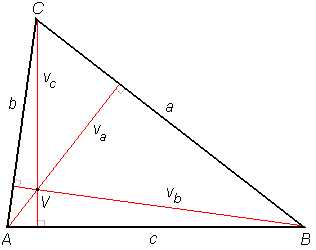
\includegraphics[scale=0.5]{Slike in skice/Visina_in_visinska_tocka.png}
            % \end{figure}
            
            \begin{figure}
                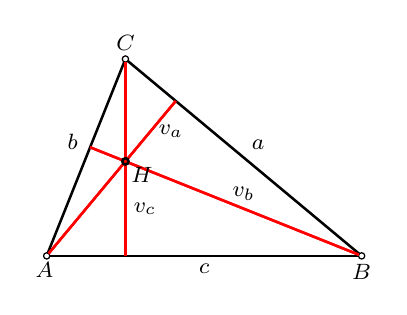
\begin{tikzpicture}
                    % \clip (0,0) rectangle (14.000000,10.000000);
                    {\footnotesize
                    
                    % Marking point A by circle
                    \draw<1-> [line width=0.016cm] (2.000000,1.500000) circle (0.040000);%
                    \draw<1-> (1.970000,1.530000) node [anchor=north] { $A$ };%
                    
                    % Marking point B by circle
                    \draw<1-> [line width=0.016cm] (6.000000,1.500000) circle (0.040000);%
                    \draw<1-> (6.000000,1.500000) node [anchor=north] { $B$ };%
                    
                    % Marking point C by circle
                    \draw<1-> [line width=0.016cm] (3.000000,4.000000) circle (0.040000);%
                    \draw<1-> (3.000000,4.000000) node [anchor=south] { $C$ };%
                    
                    % Marking point c
                    \draw<1-> (4.000000,1.500000) node [anchor=north] { $c$ };%
                    
                    % Marking point a
                    \draw<1-> (4.500000,2.750000) node [anchor=south west] { $a$ };%
                    
                    % Marking point b
                    \draw<1-> (2.500000,2.750000) node [anchor=south east] { $b$ };%
                    
                    % Marking point v_a
                    \draw<2-> (3.319672,3.083607) node [anchor=west] { $v_a$ };%
                    
                    % Marking point v_c
                    \draw<2-> (3.000000,2.100000) node [anchor=west] { $v_c$ };%
                    
                    % Marking point v_b
                    \draw<2-> (4.500000,2.100000) node [anchor=south] { $v_b$ };%
                    
                    % Drawing segment A B
                    \draw<1-> [line width=0.032cm] (2.040000,1.500000) -- (5.960000,1.500000);%
                    
                    % Drawing segment B C
                    \draw<1-> [line width=0.032cm] (5.969271,1.525607) -- (3.030729,3.974393);%
                    
                    % Drawing segment A C
                    \draw<1-> [line width=0.032cm] (2.014856,1.537139) -- (2.985144,3.962861);%
                    
                    % Changing color 255 0 0
                    \definecolor{r255g0b0}{rgb}{1.000000,0.000000,0.000000}%
                    \color{r255g0b0}% 
                    
                    % Drawing segment A A'
                    \draw<2> [line width=0.032cm] (2.025607,1.530729) -- (3.639344,3.467213);%
                    \draw<3-> [line width=0.032cm] (2.025607,1.530729) -- (2.974393,2.669271);%
                    \draw<3-> [line width=0.032cm] (3.025607,2.730729) -- (3.639344,3.467213);%
                    
                    % Drawing segment B B'
                    \draw<2> [line width=0.032cm] (5.962861,1.514856) -- (2.551724,2.879310);%
                    \draw<3-> [line width=0.032cm] (5.962861,1.514856) -- (3.037139,2.685144);%
                    \draw<3-> [line width=0.032cm] (2.962861,2.714856) -- (2.551724,2.879310);%
                    
                    % Drawing segment C C'
                    \draw<2> [line width=0.032cm] (3.000000,3.960000) -- (3.000000,1.500000);%
                    \draw<3-> [line width=0.032cm] (3.000000,3.960000) -- (3.000000,2.740000);%
                    \draw<3-> [line width=0.032cm] (3.000000,2.660000) -- (3.000000,1.500000);%
                    
                    % Changing color 0 0 0
                    \definecolor{r0g0b0}{rgb}{0.000000,0.000000,0.000000}%
                    \color{r0g0b0}% 
                    
                    % Marking point V by circle
                    \draw<3-> [line width=0.032cm] (3.000000,2.700000) circle (0.040000);%
                    \draw<3-> (2.970000,2.730000) node [anchor=north west] { $H$ };%
                    \color{black}
                    }
                \end{tikzpicture}
                    
            \end{figure}


            \end{alertblock}

            \begin{block}{Izrek}
                Nosilke vseh treh višin na stranice trikotnika se sekajo v eni točki, ki jo imenujemo \textbf{višinska točka} ali \textbf{ortocenter}.
            \end{block}
            


            \note{
                TABLA: konstrukcija višin trikotnika z ravnilom in šestilom
                \\
                DOKAZ: Skozi vsako oglišče trikotnika narišemo vzporednico k nasprotni stranici. Presečišča označimo z $A', B', C'$. Zaradi vzporednosti sta štirkotnika $ABA'C$ in $ABCB'$ paralelograma, torej je $|AB|=|A'C|$ in $|AB|=|B'C|$, iz tega $|A'C|=|B'C|$: $C$ razpolavlja $A'B'$. Podobno za $B$ in $A$. Noslike višin trikotnika $ABC$ so simmetrale stranic trikotnika $A'B'C'$. Te se sekajo v središču očrtane krožnice trikotnika $A'B'C'$, ki je višinska točka trikotnika $ABC$.

            }
        \end{frame}


        \begin{frame}

            \begin{alertblock}{Definicija}
                \textbf{Težiščnica} na stranico trikotnika je daljica, ki povezuje razpolovišče te stranice z nasprotnim ogliščem. 

            % \begin{figure}
            %     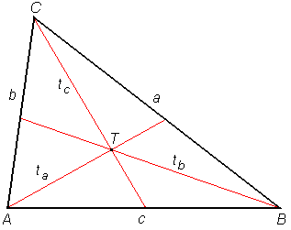
\includegraphics[scale=0.5]{Slike in skice/Teziscnice_in_tezisce.png}
            % \end{figure}

            \begin{figure}
                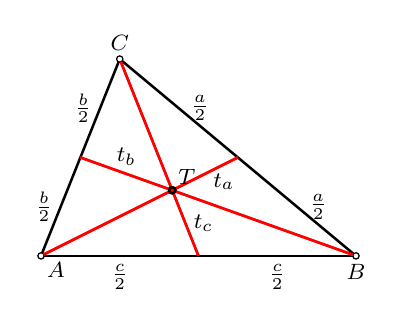
\begin{tikzpicture}
                    % \clip (0,0) rectangle (14.000000,10.000000);
                    {\footnotesize
                    
                    % Marking point A by circle
                    \draw [line width=0.016cm] (2.000000,1.500000) circle (0.040000);%
                    \draw (1.970000,1.530000) node [anchor=north west] { $A$ };%
                    
                    % Marking point B by circle
                    \draw [line width=0.016cm] (6.000000,1.500000) circle (0.040000);%
                    \draw (6.000000,1.500000) node [anchor=north] { $B$ };%
                    
                    % Marking point C by circle
                    \draw [line width=0.016cm] (3.000000,4.000000) circle (0.040000);%
                    \draw (3.000000,4.000000) node [anchor=south] { $C$ };%
                    
                    % Marking point t_a
                    \draw<2-> (4.083333,2.441667) node [anchor=west] { $t_a$ };%
                    
                    % Marking point t_c
                    \draw<2-> (3.833333,1.916667) node [anchor=west] { $t_c$ };%
                    
                    % Marking point t_b
                    \draw<2-> (3.083333,2.541667) node [anchor=south] { $t_b$ };%
                    
                    % Marking point \frac{b}{2}
                    \draw<2-> (2.250000,2.125000) node [anchor=east] { $\frac{b}{2}$ };%
                    
                    % Marking point \frac{b}{2}
                    \draw<2-> (2.750000,3.375000) node [anchor=east] { $\frac{b}{2}$ };%
                    
                    % Marking point \frac{c}{2}
                    \draw<2-> (3.000000,1.500000) node [anchor=north] { $\frac{c}{2}$ };%
                    
                    % Marking point \frac{c}{2}
                    \draw<2-> (5.000000,1.500000) node [anchor=north] { $\frac{c}{2}$ };%
                    
                    % Marking point \frac{a}{2}
                    \draw<2-> (5.30000,2.125000) node [anchor=west] { $\frac{a}{2}$ };%
                    
                    % Marking point \frac{a}{2}
                    \draw<2-> (3.80000,3.375000) node [anchor=west] { $\frac{a}{2}$ };%
                    
                    % Drawing segment A B
                    \draw [line width=0.032cm] (2.040000,1.500000) -- (5.960000,1.500000);%
                    
                    % Drawing segment B C
                    \draw [line width=0.032cm] (5.969271,1.525607) -- (3.030729,3.974393);%
                    
                    % Drawing segment A C
                    \draw [line width=0.032cm] (2.014856,1.537139) -- (2.985144,3.962861);%
                    
                    % Changing color 255 0 0
                    \definecolor{r255g0b0}{rgb}{1.000000,0.000000,0.000000}%
                    \color{r255g0b0}% 
                    
                    % Drawing segment A a
                    \draw<2> [line width=0.032cm] (2.035777,1.517889) -- (4.500000,2.750000);%
                    \draw<3-> [line width=0.032cm] (2.035777,1.517889) -- (3.630890,2.315445);%
                    \draw<3-> [line width=0.032cm] (3.702444,2.351222) -- (4.500000,2.750000);%
                    
                    % Drawing segment B b
                    \draw<2> [line width=0.032cm] (5.962330,1.513453) -- (2.500000,2.750000);%
                    \draw<3-> [line width=0.032cm] (5.962330,1.513453) -- (3.704336,2.319880);%
                    \draw<3-> [line width=0.032cm] (3.628997,2.346787) -- (2.500000,2.750000);%
                    
                    % Drawing segment C c
                    \draw<2> [line width=0.032cm] (3.014856,3.962861) -- (4.000000,1.500000);%
                    \draw<3-> [line width=0.032cm] (3.014856,3.962861) -- (3.651811,2.370472);%
                    \draw<3-> [line width=0.032cm] (3.681522,2.296194) -- (4.000000,1.500000);%
                    
                    % Changing color 0 0 0
                    \definecolor{r0g0b0}{rgb}{0.000000,0.000000,0.000000}%
                    \color{r0g0b0}% 
                    
                    % Marking point T by circle
                    \draw<3-> [line width=0.032cm] (3.666667,2.333333) circle (0.040000);%
                    \draw<3-> (3.636667,2.303333) node [anchor=south west] { $T$ };%
                    \color{black}
                    }
                \end{tikzpicture}
                    
            \end{figure}

            \end{alertblock}


            \begin{block}{Izrek}
                Vse tri trikotnikove težiščnice se sekajo v eni točki -- \textbf{težišču} ali \textbf{baricentru} trikotnika. \\ 
                Težišče deli težiščnico v razmerju $1:2$.
            \end{block}
            

            \note{
                TABLA: konstrukcija težišnic z ravnilom in šestilom
            }

        \end{frame}


        % \begin{frame}
        %     \begin{exampleblock}{Naloga 81}
        %         Konstruiraj trikotnik.
        %         \begin{itemize}
        %             \item $a=2~cm,\ b=6~cm,\ c=5~cm$;
        %             \item $c=4~cm,\ \alpha=60^\circ,\ \beta=45^\circ$;
        %             \item $a=4~cm,\ c=5~cm,\ \alpha=45^\circ$;
        %             \item $a=2,5~cm,\ c=5~cm,\ v_c=2~cm$;
        %             \item $v_c=3~cm,\ \alpha=60^\circ,\ \beta=75^\circ$;
        %             \item $v_a=2~cm,\ v_b=4~cm,\ \gamma=45^\circ$;
        %             \item $b=65~cm,\ t_b=3,5~cm,\ \gamma=60^\circ$;
        %             \item $v_a=3~cm,\ t_c=4~cm,\ \beta=45^\circ$.
        %         \end{itemize}
        %     \end{exampleblock}


        %     \note{
        %         Morda manj primerov pri nalogi 81. (b, c, h, l, n, r, š, u)
        %     }
        % \end{frame}


        \begin{frame}

            \begin{block}{Izrek}
                Simetrale vseh treh stranic trikotnika se sekajo v eni točki --  \textbf{središču trikotniku očrtane krožnice}. 

            % \begin{figure}
            %     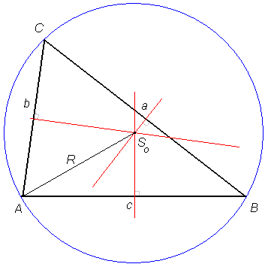
\includegraphics[scale=0.55]{Slike in skice/Trikotniku_ocrtana_kroznica.png}
            % \end{figure}

            \begin{figure}
                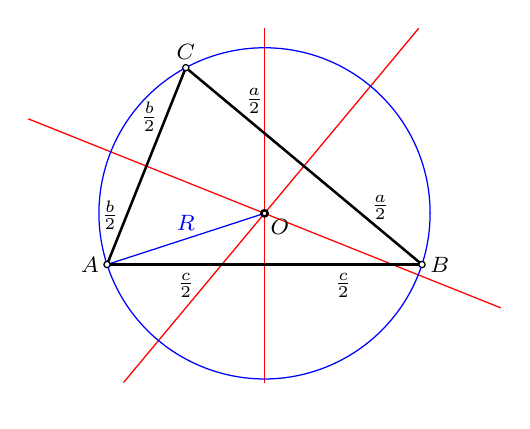
\begin{tikzpicture}
                    % \clip (0,0) rectangle (14.000000,10.000000);
                    {\footnotesize
                    
                    % Marking point A by circle
                    \draw [line width=0.016cm] (2.000000,2.500000) circle (0.040000);%
                    \draw (2.000000,2.500000) node [anchor=east] { $A$ };%
                    
                    % Marking point B by circle
                    \draw [line width=0.016cm] (6.000000,2.500000) circle (0.040000);%
                    \draw (6.000000,2.500000) node [anchor=west] { $B$ };%
                    
                    % Marking point C by circle
                    \draw [line width=0.016cm] (3.000000,5.000000) circle (0.040000);%
                    \draw (3.000000,5.000000) node [anchor=south] { $C$ };%
                    
                    % Marking point \frac{b}{2}
                    \draw (2.250000,3.125000) node [anchor=east] { $\frac{b}{2}$ };%
                    
                    % Marking point \frac{b}{2}
                    \draw (2.750000,4.375000) node [anchor=east] { $\frac{b}{2}$ };%
                    
                    % Marking point \frac{c}{2}
                    \draw (3.000000,2.500000) node [anchor=north] { $\frac{c}{2}$ };%
                    
                    % Marking point \frac{c}{2}
                    \draw (5.000000,2.500000) node [anchor=north] { $\frac{c}{2}$ };%
                    
                    % Marking point \frac{a}{2}
                    \draw (5.250000,3.225000) node [anchor=west] { $\frac{a}{2}$ };%
                    
                    % Marking point \frac{a}{2}
                    \draw (3.650000,4.575000) node [anchor=west] { $\frac{a}{2}$ };%
                    
                    % Changing color 255 0 0
                    \definecolor{r255g0b0}{rgb}{1.000000,0.000000,0.000000}%
                    \color{r255g0b0}% 
                    
                    % Drawing line s_c
                    \draw [line width=0.016cm] (4.000000,1.000000) -- (4.000000,3.110000);%
                    \draw [line width=0.016cm] (4.000000,3.190000) -- (4.000000,5.500000);%
                    
                    % Drawing line s_a
                    \draw [line width=0.016cm] (2.208333,1.000000) -- (3.974393,3.119271);%
                    \draw [line width=0.016cm] (4.025607,3.180729) -- (5.958333,5.500000);%
                    
                    % Drawing line s_b
                    \draw [line width=0.016cm] (1.000000,4.350000) -- (3.962861,3.164856);%
                    \draw [line width=0.016cm] (4.037139,3.135144) -- (7.000000,1.950000);%
                    
                    % Changing color 0 0 255
                    \definecolor{r0g0b255}{rgb}{0.000000,0.000000,1.000000}%
                    \color{r0g0b255}% 
                    
                    % Drawing circle S_O A
                    \draw [line width=0.016cm] (2.012724,2.462079) -- (2.023851,2.430741) arc (200:340:2.102974 and 2.102974) -- (5.987275,2.462077);%
                    \draw [line width=0.016cm] (6.012001,2.538157) -- (6.021508,2.570341) arc (344:360:2.102974 and 2.102974) --(6.102974,3.150000) arc (0:117:2.102974 and 2.102974) -- (3.035368,5.018685);%
                    \draw [line width=0.016cm] (2.964994,4.980646) -- (2.948513,4.971229) arc (120:196:2.102974 and 2.102974) -- (1.987999,2.538158);%
                    
                    % Drawing segment A S_O
                    \draw [line width=0.016cm] (2.038041,2.512363) -- (3.961959,3.137637);%
                    
                    % Marking point R
                    \draw (3.000000,2.825000) node [anchor=south] { $R$ };%
                    
                    % Changing color 0 0 0
                    \definecolor{r0g0b0}{rgb}{0.000000,0.000000,0.000000}%
                    \color{r0g0b0}% 
                    
                    % Drawing segment A B
                    \draw [line width=0.032cm] (2.040000,2.500000) -- (5.960000,2.500000);%
                    
                    % Drawing segment B C
                    \draw [line width=0.032cm] (5.969271,2.525607) -- (3.030729,4.974393);%
                    
                    % Drawing segment A C
                    \draw [line width=0.032cm] (2.014856,2.537139) -- (2.985144,4.962861);%
                    
                    % Marking point S_O by circle
                    \draw [line width=0.032cm] (4.000000,3.150000) circle (0.040000);%
                    \draw (3.970000,3.180000) node [anchor=north west] { $O$ };%
                    \color{black}
                    }
                \end{tikzpicture}    

            \end{figure}

            \end{block}


            \begin{block}{}
                Očrtana krožnica poteka skozi vsa oglišča trikotnika. Vse stranice trikotnika so tetive krožnice.
            \end{block}


            \note{
                TABLA: konstrukcija simetral stranic in očrtane krožnice z ravnilom in šestilom
                \\
                DOKAZ: Konstruiramo simetrali stranic $AC$ in $AB$. Vsaka točka na njiju je enako oddaljena od oglišč stranice. Torej je njuno presečišče $S_O$ enako oddalje od vseh trh oglišč $A, B, C$ in tako središče trikotniku očrtane krožnice. Podbno za simetralo strannice $BC$.
            }
        \end{frame}


        \begin{frame}

            \begin{block}{Izrek}
                Simetrale notranjih kotov trikotnika se sekajo v eni točki. Ta točka je \textbf{središče trikotniku včrtane krožnice}.

            % \begin{figure}
            %     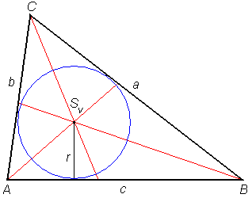
\includegraphics[scale=0.65]{Slike in skice/Trikotniku_vcrtana_kroznica.png}
            % \end{figure}

            \begin{figure}
                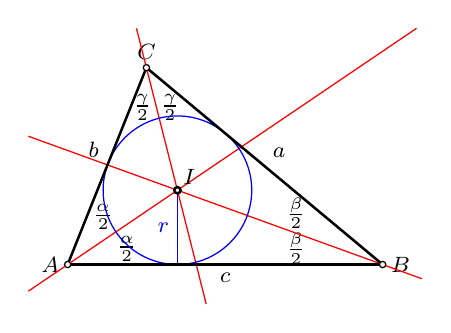
\begin{tikzpicture}
                    % \clip (0,0) rectangle (14.000000,10.000000);
                    {\footnotesize
                    
                    % Marking point A by circle
                    \draw [line width=0.016cm] (2.000000,2.500000) circle (0.040000);%
                    \draw (2.000000,2.500000) node [anchor=east] { $A$ };%
                    
                    % Marking point B by circle
                    \draw [line width=0.016cm] (6.000000,2.500000) circle (0.040000);%
                    \draw (6.000000,2.500000) node [anchor=west] { $B$ };%
                    
                    % Marking point C by circle
                    \draw [line width=0.016cm] (3.000000,5.000000) circle (0.040000);%
                    \draw (3.000000,5.000000) node [anchor=south] { $C$ };%
                    
                    % Marking point b
                    \draw (2.500000,3.750000) node [anchor=south east] { $b$ };%
                    
                    % Marking point c
                    \draw (4.000000,2.500000) node [anchor=north] { $c$ };%
                    
                    % Marking point a
                    \draw (4.500000,3.750000) node [anchor=south west] { $a$ };%
                    
                    % Marking point \frac{\alpha}{2}
                    \draw (2.750000,2.700000) node  { $\frac{\alpha}{2}$ };%
                    
                    % Marking point \frac{\gamma}{2}
                    \draw (2.950000,4.500000) node  { $\frac{\gamma}{2}$ };%
                    
                    % Marking point \frac{\alpha}{2}
                    \draw (2.450000,3.100000) node  { $\frac{\alpha}{2}$ };%
                    
                    % Marking point \frac{\beta}{2}
                    \draw (4.900000,2.700000) node  { $\frac{\beta}{2}$ };%
                    
                    % Marking point \frac{\beta}{2}
                    \draw (4.900000,3.150000) node  { $\frac{\beta}{2}$ };%
                    
                    % Marking point \frac{\gamma}{2}
                    \draw (3.300000,4.500000) node  { $\frac{\gamma}{2}$ };%
                    
                    % Changing color 255 0 0
                    \definecolor{r255g0b0}{rgb}{1.000000,0.000000,0.000000}%
                    \color{r255g0b0}% 
                    
                    % Drawing line s_c
                    \draw [line width=0.016cm] (3.758922,2.000000) -- (3.403539,3.404822);%
                    \draw [line width=0.016cm] (3.383919,3.482379) -- (3.009810,4.961222);%
                    \draw [line width=0.016cm] (2.990190,5.038778) -- (2.873513,5.500000);%
                    
                    % Drawing line s_a
                    \draw [line width=0.016cm] (6.431099,5.500000) -- (3.426851,3.466025);%
                    \draw [line width=0.016cm] (3.360606,3.421175) -- (2.033123,2.522425);%
                    \draw [line width=0.016cm] (1.966877,2.477575) -- (1.500000,2.161484);%
                    
                    % Drawing line s_b
                    \draw [line width=0.016cm] (1.500000,4.129225) -- (3.356118,3.457217);%
                    \draw [line width=0.016cm] (3.431340,3.429983) -- (5.962389,2.513617);%
                    \draw [line width=0.016cm] (6.037611,2.486383) -- (6.500000,2.318975);%
                    
                    % Changing color 0 0 255
                    \definecolor{r0g0b255}{rgb}{0.000000,0.000000,1.000000}%
                    \color{r0g0b255}% 
                    
                    % Drawing circle S_V X
                    \draw [line width=0.016cm] (3.393729,3.443600) circle (0.943600);%
                    
                    % Drawing segment X S_V
                    \draw [line width=0.016cm] (3.393729,2.500000) -- (3.393729,3.403600);%
                    
                    % Marking point r
                    \draw (3.393729,2.971800) node [anchor=east] { $r$ };%
                    
                    % Changing color 0 0 0
                    \definecolor{r0g0b0}{rgb}{0.000000,0.000000,0.000000}%
                    \color{r0g0b0}% 
                    
                    % Drawing segment A B
                    \draw [line width=0.032cm] (2.040000,2.500000) -- (5.960000,2.500000);%
                    
                    % Drawing segment B C
                    \draw [line width=0.032cm] (5.969271,2.525607) -- (3.030729,4.974393);%
                    
                    % Drawing segment A C
                    \draw [line width=0.032cm] (2.014856,2.537139) -- (2.985144,4.962861);%
                    
                    % Marking point S_V by circle
                    \draw [line width=0.032cm] (3.393729,3.443600) circle (0.040000);%
                    \draw (3.363729,3.413600) node [anchor=south west] { $I$ };%
                    \color{black}
                    }
                \end{tikzpicture}
                    
            \end{figure}

            \end{block}


            \begin{block}{}
               Včrtana krožnica ima vse tri stranice trikotnika za tangente.
            \end{block}


            \note{
                TABLA: konstrukcija simetral kotov in včrtane krožnice z ravnilom in šestilom
                \\
                DOKAZ: Narišemo simetrali kotov pri $A$ in $B$. Vsaka točka na njiju je enako oddaljena od nosilk stranic ob kotu. Njuno presečišče $S_V$ je torej enako oddalje od vseh treh nosilk stranic trikotnika. In zatorej je središče krožnice, ki se dotika vseh treh stranic -- trikotniku včrtane krožnice.
            }
        \end{frame}

        % \begin{frame}
        %     \begin{exampleblock}{Naloga 83}
        %         Dan je trikotnik $\triangle ABC$ s podatki $b=5~cm,\ \beta=45^\circ,\ \gamma=60^\circ$.
        %         \begin{enumerate}
        %             \item Konstruiraj trikotnik $\triangle ABC$.
        %             \item Konstruiraj trikotniku $\triangle ABC$ očrtano krožnico.
        %             \item Koliko je velik zunanji kot pri oglišču $A$?
        %         \end{enumerate}
        %     \end{exampleblock}

        %     \pause
        %     \begin{exampleblock}{Naloga 84}
        %         Dan je trikotnik $\triangle ABC$ s podatki $a=5~cm,\ c=4~cm,\ t_c=4~cm$.
        %         \begin{enumerate}
        %             \item Konstruiraj trikotnik $\triangle ABC$.
        %             \item Konstruiraj trikotniku $\triangle ABC$ včrtano krožnico.
        %             \item Kateri izmed $\angle BAC$ in $\angle ACB$ je večji? Utemelji (brez merjenja).
        %         \end{enumerate}
        %     \end{exampleblock}
        % \end{frame}


        \begin{frame}

            \begin{block}{}
                Težišče, središče trikotniku očrtane kroznice, središče trikotniku včrtane krožnice in višinska točka so \textbf{znamenite točke trikotnika}.
            \end{block}

            
            \begin{block}{Izrek}
                Višinska točka, središče očrtane krožnice in težišče so vedno kolinearne. Premico, ki jih povezuje, imenujemo \textbf{Eulerjeva premica}.

            % \begin{figure}
            %     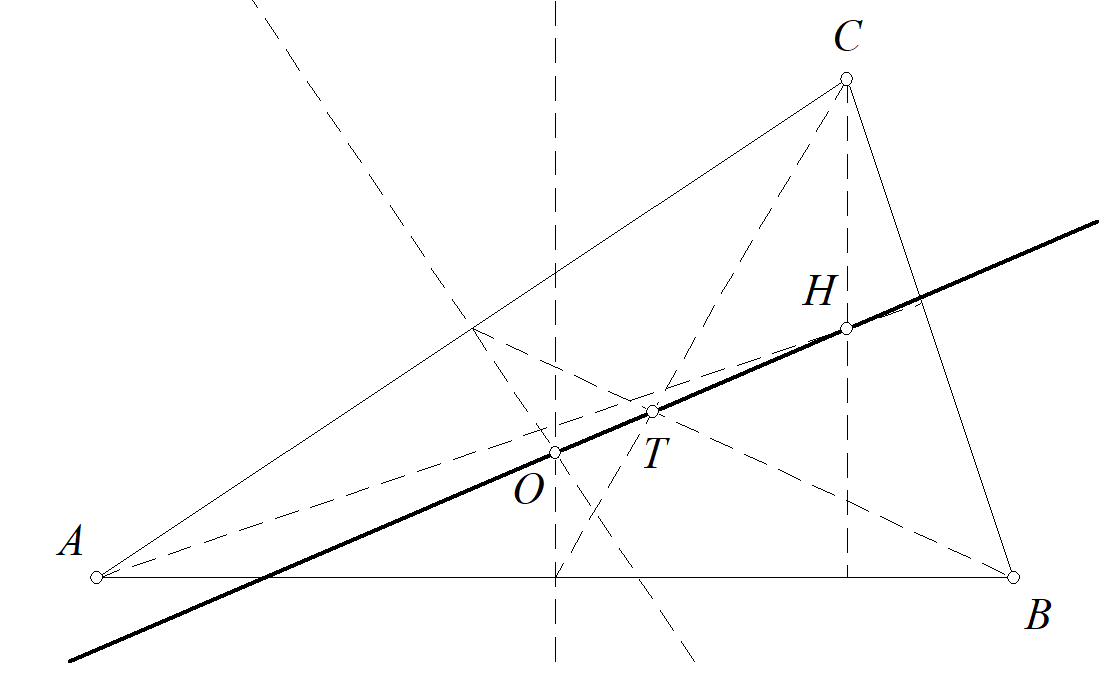
\includegraphics[scale=0.23]{Slike in skice/Eulerjeva_premica.png}
            % \end{figure}

                \begin{figure}
                    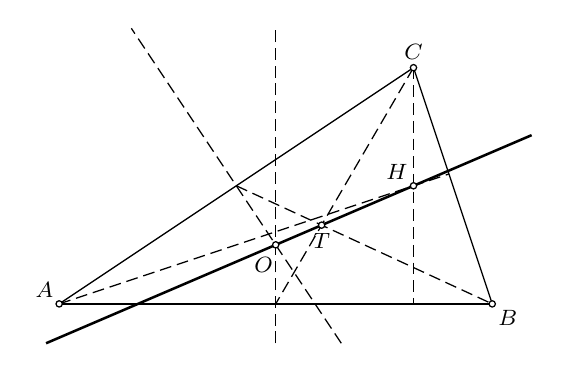
\begin{tikzpicture}
                        % \clip (0,0) rectangle (14.000000,10.000000);
                        {\footnotesize
                        
                        % Drawing segment A B
                        \draw [line width=0.016cm] (1.540000,3.500000) -- (6.960000,3.500000);%
                        
                        % Drawing segment A C
                        \draw [line width=0.016cm] (1.533282,3.522188) -- (5.966718,6.477812);%
                        
                        % Drawing segment B C
                        \draw [line width=0.016cm] (6.987351,3.537947) -- (6.012649,6.462053);%
                        
                        % Drawing line b
                        \draw [line width=0.016cm] (5.083333,3.000000) -- (5.000128,3.124808);%
                        \draw [line width=0.016cm] (4.958526,3.187211) -- (4.875321,3.312019);%
                        \draw [line width=0.016cm] (4.833718,3.374423) -- (4.750513,3.499230);%
                        \draw [line width=0.016cm] (4.708911,3.561634) -- (4.625706,3.686441);%
                        \draw [line width=0.016cm] (4.584103,3.748845) -- (4.500898,3.873653);%
                        \draw [line width=0.016cm] (4.459296,3.936057) -- (4.376091,4.060864);%
                        \draw [line width=0.016cm] (4.334488,4.123268) -- (4.272188,4.216718);%
                        \draw [line width=0.016cm] (4.209681,4.310479) -- (4.126475,4.435287);%
                        \draw [line width=0.016cm] (4.084873,4.497691) -- (4.001668,4.622498);%
                        \draw [line width=0.016cm] (3.960065,4.684902) -- (3.876860,4.809709);%
                        \draw [line width=0.016cm] (3.835258,4.872113) -- (3.752053,4.996921);%
                        \draw [line width=0.016cm] (3.710450,5.059324) -- (3.627245,5.184132);%
                        \draw [line width=0.016cm] (3.585643,5.246536) -- (3.502438,5.371343);%
                        \draw [line width=0.016cm] (3.460835,5.433747) -- (3.377630,5.558555);%
                        \draw [line width=0.016cm] (3.336028,5.620958) -- (3.252823,5.745766);%
                        \draw [line width=0.016cm] (3.211220,5.808170) -- (3.128015,5.932977);%
                        \draw [line width=0.016cm] (3.086413,5.995381) -- (3.003208,6.120189);%
                        \draw [line width=0.016cm] (2.961605,6.182592) -- (2.878400,6.307400);%
                        \draw [line width=0.016cm] (2.836798,6.369804) -- (2.753593,6.494611);%
                        \draw [line width=0.016cm] (2.711990,6.557015) -- (2.628785,6.681823);%
                        \draw [line width=0.016cm] (2.587182,6.744226) -- (2.503977,6.869034);%
                        \draw [line width=0.016cm] (2.462375,6.931438) -- (2.416667,7.000000);%
                        
                        % Drawing line c
                        \draw [line width=0.016cm] (4.250000,3.000000) -- (4.250000,3.150000);%
                        \draw [line width=0.016cm] (4.250000,3.225000) -- (4.250000,3.375000);%
                        \draw [line width=0.016cm] (4.250000,3.450000) -- (4.250000,3.600000);%
                        \draw [line width=0.016cm] (4.250000,3.675000) -- (4.250000,3.825000);%
                        \draw [line width=0.016cm] (4.250000,3.900000) -- (4.250000,4.050000);%
                        \draw [line width=0.016cm] (4.250000,4.125000) -- (4.250000,4.210000);%
                        \draw [line width=0.016cm] (4.250000,4.350000) -- (4.250000,4.500000);%
                        \draw [line width=0.016cm] (4.250000,4.575000) -- (4.250000,4.725000);%
                        \draw [line width=0.016cm] (4.250000,4.800000) -- (4.250000,4.950000);%
                        \draw [line width=0.016cm] (4.250000,5.025000) -- (4.250000,5.175000);%
                        \draw [line width=0.016cm] (4.250000,5.250000) -- (4.250000,5.400000);%
                        \draw [line width=0.016cm] (4.250000,5.475000) -- (4.250000,5.625000);%
                        \draw [line width=0.016cm] (4.250000,5.700000) -- (4.250000,5.850000);%
                        \draw [line width=0.016cm] (4.250000,5.925000) -- (4.250000,6.075000);%
                        \draw [line width=0.016cm] (4.250000,6.150000) -- (4.250000,6.300000);%
                        \draw [line width=0.016cm] (4.250000,6.375000) -- (4.250000,6.525000);%
                        \draw [line width=0.016cm] (4.250000,6.600000) -- (4.250000,6.750000);%
                        \draw [line width=0.016cm] (4.250000,6.825000) -- (4.250000,6.975000);%
                        
                        % Drawing segment C C'
                        \draw [line width=0.016cm] (5.979845,6.465449) -- (5.924419,6.370433);%
                        \draw [line width=0.016cm] (5.886629,6.305650) -- (5.811048,6.176083);%
                        \draw [line width=0.016cm] (5.773258,6.111299) -- (5.697677,5.981733);%
                        \draw [line width=0.016cm] (5.659887,5.916949) -- (5.584306,5.787382);%
                        \draw [line width=0.016cm] (5.546516,5.722599) -- (5.470935,5.593032);%
                        \draw [line width=0.016cm] (5.433145,5.528249) -- (5.357564,5.398682);%
                        \draw [line width=0.016cm] (5.319774,5.333898) -- (5.244193,5.204332);%
                        \draw [line width=0.016cm] (5.206403,5.139548) -- (5.130822,5.009981);%
                        \draw [line width=0.016cm] (5.093032,4.945198) -- (5.017452,4.815631);%
                        \draw [line width=0.016cm] (4.979661,4.750848) -- (4.904081,4.621281);%
                        \draw [line width=0.016cm] (4.866290,4.556497) -- (4.853488,4.534551);%
                        \draw [line width=0.016cm] (4.813178,4.465449) -- (4.790710,4.426931);%
                        \draw [line width=0.016cm] (4.752919,4.362147) -- (4.677339,4.232580);%
                        \draw [line width=0.016cm] (4.639548,4.167797) -- (4.563968,4.038230);%
                        \draw [line width=0.016cm] (4.526177,3.973447) -- (4.450597,3.843880);%
                        \draw [line width=0.016cm] (4.412806,3.779096) -- (4.337226,3.649530);%
                        \draw [line width=0.016cm] (4.299435,3.584746) -- (4.250000,3.500000);%
                        
                        % Drawing segment C U
                        \draw [line width=0.016cm] (6.000000,6.460000) -- (6.000000,6.350000);%
                        \draw [line width=0.016cm] (6.000000,6.275000) -- (6.000000,6.125000);%
                        \draw [line width=0.016cm] (6.000000,6.050000) -- (6.000000,5.900000);%
                        \draw [line width=0.016cm] (6.000000,5.825000) -- (6.000000,5.675000);%
                        \draw [line width=0.016cm] (6.000000,5.600000) -- (6.000000,5.450000);%
                        \draw [line width=0.016cm] (6.000000,5.375000) -- (6.000000,5.225000);%
                        \draw [line width=0.016cm] (6.000000,5.150000) -- (6.000000,5.040000);%
                        \draw [line width=0.016cm] (6.000000,4.925000) -- (6.000000,4.775000);%
                        \draw [line width=0.016cm] (6.000000,4.700000) -- (6.000000,4.550000);%
                        \draw [line width=0.016cm] (6.000000,4.475000) -- (6.000000,4.325000);%
                        \draw [line width=0.016cm] (6.000000,4.250000) -- (6.000000,4.100000);%
                        \draw [line width=0.016cm] (6.000000,4.025000) -- (6.000000,3.875000);%
                        \draw [line width=0.016cm] (6.000000,3.800000) -- (6.000000,3.650000);%
                        \draw [line width=0.016cm] (6.000000,3.575000) -- (6.000000,3.500000);%
                        
                        % Drawing segment A V
                        \draw [line width=0.016cm] (1.537947,3.512649) -- (1.642302,3.547434);%
                        \draw [line width=0.016cm] (1.713454,3.571151) -- (1.855756,3.618585);%
                        \draw [line width=0.016cm] (1.926907,3.642302) -- (2.069210,3.689737);%
                        \draw [line width=0.016cm] (2.140361,3.713454) -- (2.282664,3.760888);%
                        \draw [line width=0.016cm] (2.353815,3.784605) -- (2.496117,3.832039);%
                        \draw [line width=0.016cm] (2.567269,3.855756) -- (2.709571,3.903190);%
                        \draw [line width=0.016cm] (2.780722,3.926907) -- (2.923025,3.974342);%
                        \draw [line width=0.016cm] (2.994176,3.998059) -- (3.136479,4.045493);%
                        \draw [line width=0.016cm] (3.207630,4.069210) -- (3.349932,4.116644);%
                        \draw [line width=0.016cm] (3.421084,4.140361) -- (3.563386,4.187795);%
                        \draw [line width=0.016cm] (3.634537,4.211512) -- (3.776840,4.258947);%
                        \draw [line width=0.016cm] (3.847991,4.282664) -- (3.990294,4.330098);%
                        \draw [line width=0.016cm] (4.061445,4.353815) -- (4.203747,4.401249);%
                        \draw [line width=0.016cm] (4.274899,4.424966) -- (4.417201,4.472400);%
                        \draw [line width=0.016cm] (4.488352,4.496117) -- (4.630655,4.543552);%
                        \draw [line width=0.016cm] (4.701806,4.567269) -- (4.844109,4.614703);%
                        \draw [line width=0.016cm] (4.915260,4.638420) -- (5.057562,4.685854);%
                        \draw [line width=0.016cm] (5.128714,4.709571) -- (5.271016,4.757005);%
                        \draw [line width=0.016cm] (5.342167,4.780722) -- (5.484470,4.828157);%
                        \draw [line width=0.016cm] (5.555621,4.851874) -- (5.697924,4.899308);%
                        \draw [line width=0.016cm] (5.769075,4.923025) -- (5.911377,4.970459);%
                        \draw [line width=0.016cm] (6.037947,5.012649) -- (6.124831,5.041610);%
                        \draw [line width=0.016cm] (6.195982,5.065327) -- (6.338285,5.112762);%
                        \draw [line width=0.016cm] (6.409436,5.136479) -- (6.450000,5.150000);%
                        
                        % Drawing segment B' B
                        \draw [line width=0.016cm] (3.750000,5.000000) -- (3.886194,4.937141);%
                        \draw [line width=0.016cm] (3.954291,4.905712) -- (4.090485,4.842853);%
                        \draw [line width=0.016cm] (4.158582,4.811424) -- (4.294776,4.748565);%
                        \draw [line width=0.016cm] (4.362873,4.717136) -- (4.499066,4.654277);%
                        \draw [line width=0.016cm] (4.567163,4.622848) -- (4.703357,4.559989);%
                        \draw [line width=0.016cm] (4.771454,4.528560) -- (4.797015,4.516762);%
                        \draw [line width=0.016cm] (4.869652,4.483238) -- (4.907648,4.465701);%
                        \draw [line width=0.016cm] (4.975745,4.434271) -- (5.111939,4.371413);%
                        \draw [line width=0.016cm] (5.180036,4.339983) -- (5.316230,4.277125);%
                        \draw [line width=0.016cm] (5.384327,4.245695) -- (5.520521,4.182837);%
                        \draw [line width=0.016cm] (5.588618,4.151407) -- (5.724812,4.088548);%
                        \draw [line width=0.016cm] (5.792909,4.057119) -- (5.929103,3.994260);%
                        \draw [line width=0.016cm] (5.997199,3.962831) -- (6.133393,3.899972);%
                        \draw [line width=0.016cm] (6.201490,3.868543) -- (6.337684,3.805684);%
                        \draw [line width=0.016cm] (6.405781,3.774255) -- (6.541975,3.711396);%
                        \draw [line width=0.016cm] (6.610072,3.679967) -- (6.746266,3.617108);%
                        \draw [line width=0.016cm] (6.814363,3.585679) -- (6.950557,3.522820);%
                        
                        % Marking point A by circle
                        \draw [line width=0.016cm] (1.500000,3.500000) circle (0.040000);%
                        \draw (1.530000,3.470000) node [anchor=south east] { $A$ };%
                        
                        % Marking point B by circle
                        \draw [line width=0.016cm] (7.000000,3.500000) circle (0.040000);%
                        \draw (6.970000,3.530000) node [anchor=north west] { $B$ };%
                        
                        % Marking point C by circle
                        \draw [line width=0.016cm] (6.000000,6.500000) circle (0.040000);%
                        \draw (6.000000,6.500000) node [anchor=south] { $C$ };%
                        
                        % Marking point O by circle
                        \draw [line width=0.016cm] (4.250000,4.250000) circle (0.040000);%
                        \draw (4.320000,4.200000) node [anchor=north east] { $O$ };%
                        
                        % Marking point T by circle
                        \draw [line width=0.016cm] (4.833333,4.500000) circle (0.040000);%
                        \draw (4.833333,4.500000) node [anchor=north] { $T$ };%
                        
                        % Marking point H_C by circle
                        \draw [line width=0.016cm] (6.000000,5.000000) circle (0.040000);%
                        \draw (6.030000,4.970000) node [anchor=south east] { $H$ };%
                        
                        % Drawing line O T
                        \draw [line width=0.032cm] (1.333333,3.000000) -- (4.213234,4.234243);%
                        \draw [line width=0.032cm] (4.286766,4.265757) -- (4.796568,4.484243);%
                        \draw [line width=0.032cm] (4.870099,4.515757) -- (5.963234,4.984243);%
                        \draw [line width=0.032cm] (6.036766,5.015757) -- (7.500000,5.642857);%
                        }
                    \end{tikzpicture}
                        
                \end{figure}

            \end{block}

        \end{frame}





        \begin{frame}
            \large\textbf{Vrste trikotnikov -- glede na stranice}
            % ~\\
            \normalsize
            \begin{columns}
                \column<2->{0.35\textwidth}
                \begin{exampleblock}{}
                    RAZNOSTRANIČNI TRIKOTNIK 

                    \begin{figure}
                        \begin{tikzpicture}
                            % \clip (0,0) rectangle (14.000000,10.000000);
                            {\footnotesize
                            
                            % Marking point A by circle
                            \draw [line width=0.016cm] (1.500000,1.500000) circle (0.040000);%
                            \draw (1.500000,1.500000) node [anchor=north] { $A$ };%
                            
                            % Marking point B by circle
                            \draw [line width=0.016cm] (6.000000,1.500000) circle (0.040000);%
                            \draw (6.000000,1.500000) node [anchor=north] { $B$ };%
                            
                            % Marking point C by circle
                            \draw [line width=0.016cm] (4.500000,4.500000) circle (0.040000);%
                            \draw (4.500000,4.500000) node [anchor=south] { $C$ };%
                            
                            % Changing color 255 0 0
                            \definecolor{r255g0b0}{rgb}{1.000000,0.000000,0.000000}%
                            \color{r255g0b0}% 
                            
                            % Drawing segment B C
                            \draw [line width=0.016cm] (5.982111,1.535777) -- (4.517889,4.464223);%
                            
                            % Marking point a
                            \draw (5.250000,3.000000) node [anchor=south west] { $a$ };%
                            
                            % Changing color 0 255 0
                            \definecolor{r0g255b0}{rgb}{0.000000,1.000000,0.000000}%
                            \color{r0g255b0}% 
                            
                            % Drawing segment A C
                            \draw [line width=0.016cm] (1.528284,1.528284) -- (4.471716,4.471716);%
                            
                            % Marking point b
                            \draw (3.000000,3.000000) node [anchor=south east] { $b$ };%
                            
                            % Changing color 0 0 255
                            \definecolor{r0g0b255}{rgb}{0.000000,0.000000,1.000000}%
                            \color{r0g0b255}% 
                            
                            % Drawing segment A B
                            \draw [line width=0.016cm] (1.540000,1.500000) -- (5.960000,1.500000);%
                            
                            % Marking point c
                            \draw (3.750000,1.500000) node [anchor=north] { $c$ };%
                            \color{black}
                            }
                        \end{tikzpicture}
                            
                    \end{figure}

                    vse tri stranice različno dolge 
                    % $\Rightarrow$ vsi trije koti so različni
                    
                \end{exampleblock}
                \column<3->{0.27\textwidth}
                \begin{exampleblock}{}
                    ENAKOKRAKI TRIKOTNIK 

                    \begin{figure}
                        \begin{tikzpicture}
                            % \clip (0,0) rectangle (14.000000,10.000000);
                            {\footnotesize
                            
                            % Marking point A by circle
                            \draw [line width=0.016cm] (1.500000,1.500000) circle (0.040000);%
                            \draw (1.500000,1.500000) node [anchor=north] { $A$ };%
                            
                            % Marking point B by circle
                            \draw [line width=0.016cm] (5.000000,1.500000) circle (0.040000);%
                            \draw (5.000000,1.500000) node [anchor=north] { $B$ };%
                            
                            % Marking point C by circle
                            \draw [line width=0.016cm] (3.250000,5.000000) circle (0.040000);%
                            \draw (3.250000,5.000000) node [anchor=south] { $C$ };%
                            
                            % Changing color 255 0 0
                            \definecolor{r255g0b0}{rgb}{1.000000,0.000000,0.000000}%
                            \color{r255g0b0}% 
                            
                            % Drawing segment B C
                            \draw [line width=0.016cm] (4.982111,1.535777) -- (3.267889,4.964223);%
                            
                            % Marking point a
                            \draw (4.125000,3.250000) node [anchor=south west] { $a$ };%
                            
                            % Drawing segment A C
                            \draw [line width=0.016cm] (1.517889,1.535777) -- (3.232111,4.964223);%
                            
                            % Marking point a
                            \draw (2.375000,3.250000) node [anchor=south east] { $a$ };%
                            
                            % Changing color 0 0 255
                            \definecolor{r0g0b255}{rgb}{0.000000,0.000000,1.000000}%
                            \color{r0g0b255}% 
                            
                            % Drawing segment A B
                            \draw [line width=0.016cm] (1.540000,1.500000) -- (4.960000,1.500000);%
                            
                            % Marking point c
                            \draw (3.250000,1.500000) node [anchor=north] { $c$ };%
                            \color{black}
                            }
                        \end{tikzpicture}
                            
                    \end{figure}

                    dve stranici enako dolgi 
                    % $\Rightarrow$ kota ob osnovnici sta skladna
                    
                \end{exampleblock}                
                \column<4->{0.31\textwidth}
                \begin{exampleblock}{}
                    ENAKOSTRANIČNI ali PRAVILNI TRIKOTNIK 

                    \begin{figure}
                        \begin{tikzpicture}
                            % \clip (0,0) rectangle (14.000000,10.000000);
                            {\footnotesize
                            
                            % Marking point A by circle
                            \draw [line width=0.016cm] (1.500000,1.500000) circle (0.040000);%
                            \draw (1.500000,1.500000) node [anchor=north] { $A$ };%
                            
                            % Marking point B by circle
                            \draw [line width=0.016cm] (5.500000,1.500000) circle (0.040000);%
                            \draw (5.500000,1.500000) node [anchor=north] { $B$ };%
                            
                            % Marking point C by circle
                            \draw [line width=0.016cm] (3.500000,5.000000) circle (0.040000);%
                            \draw (3.500000,5.000000) node [anchor=south] { $C$ };%
                            
                            % Changing color 0 255 0
                            \definecolor{r0g255b0}{rgb}{0.000000,1.000000,0.000000}%
                            \color{r0g255b0}% 
                            
                            % Drawing segment B C
                            \draw [line width=0.016cm] (5.480154,1.534730) -- (3.519846,4.965270);%
                            
                            % Marking point a
                            \draw (4.500000,3.250000) node [anchor=south west] { $a$ };%
                            
                            % Drawing segment A C
                            \draw [line width=0.016cm] (1.519846,1.534730) -- (3.480154,4.965270);%
                            
                            % Marking point a
                            \draw (2.500000,3.250000) node [anchor=south east] { $a$ };%
                            
                            % Drawing segment A B
                            \draw [line width=0.016cm] (1.540000,1.500000) -- (5.460000,1.500000);%
                            
                            % Marking point a
                            \draw (3.500000,1.500000) node [anchor=north] { $a$ };%
                            \color{black}
                            }
                        \end{tikzpicture}
                            
                    \end{figure}

                    vse tri stranice enako dolge 
                    % $\Rightarrow$ vsi trije koti so skladni
                    
                \end{exampleblock}            
            \end{columns}


            \note{
                Enakostranični trikotnik: vse znamenite točke in daljice sovpadajo.
                
                Enakokraki trikotnik: znamenite točke so kolinearne; simetrali osnovnice in kota ob vrhu ter višina in težiščnica osnovnice sovpadajo.
            }
        \end{frame}

        \begin{frame}
            \large\textbf{Vrste trikotnikov -- glede na kote}
            % ~\\
            \normalsize
            \begin{columns}
                \column<2->{0.35\textwidth}
                \begin{exampleblock}{}
                    OSTROKOTNI TRIKOTNIK 

                    \begin{figure}
                        \begin{tikzpicture}
                            % \clip (0,0) rectangle (14.000000,10.000000);
                            {\footnotesize
                            
                            % Marking point A by circle
                            \draw [line width=0.016cm] (1.500000,1.500000) circle (0.040000);%
                            \draw (1.500000,1.500000) node [anchor=north] { $A$ };%
                            
                            % Marking point B by circle
                            \draw [line width=0.016cm] (6.000000,1.500000) circle (0.040000);%
                            \draw (6.000000,1.500000) node [anchor=north] { $B$ };%
                            
                            % Marking point C by circle
                            \draw [line width=0.016cm] (4.500000,4.500000) circle (0.040000);%
                            \draw (4.500000,4.500000) node [anchor=south] { $C$ };%
                            
                            % Drawing segment A B
                            \draw [line width=0.016cm] (1.540000,1.500000) -- (5.960000,1.500000);%
                            
                            % Drawing segment A C
                            \draw [line width=0.016cm] (1.528284,1.528284) -- (4.471716,4.471716);%
                            
                            % Drawing segment B C
                            \draw [line width=0.016cm] (5.982111,1.535777) -- (4.517889,4.464223);%
                            
                            % Changing color 0 0 255
                            \definecolor{r0g0b255}{rgb}{0.000000,0.000000,1.000000}%
                            \color{r0g0b255}% 
                            
                            % Marking point \gamma
                            \draw (4.400000,4.200000) node [anchor=north] { $\gamma$ };%
                            
                            % Marking point \alpha
                            \draw (1.800000,1.500000) node [anchor=south west] { $\alpha$ };%
                            
                            % Marking point \beta
                            \draw (5.800000,1.500000) node [anchor=south east] { $\beta$ };%
                            \color{black}
                            }
                        \end{tikzpicture}
                            
                    \end{figure}

                    ima tri ostre notranje kote
                    
                \end{exampleblock}
                \column<3->{0.29\textwidth}
                \begin{exampleblock}{}
                    TOPOKOTNI TRIKOTNIK 

                    \begin{figure}
                        \begin{tikzpicture}
                            % \clip (0,0) rectangle (14.000000,10.000000);
                            {\footnotesize
                            
                            % Marking point A by circle
                            \draw [line width=0.016cm] (1.500000,1.500000) circle (0.040000);%
                            \draw (1.500000,1.500000) node [anchor=north] { $A$ };%
                            
                            % Marking point B by circle
                            \draw [line width=0.016cm] (4.000000,1.500000) circle (0.040000);%
                            \draw (4.000000,1.500000) node [anchor=north] { $B$ };%
                            
                            % Marking point C by circle
                            \draw [line width=0.016cm] (5.000000,4.000000) circle (0.040000);%
                            \draw (5.000000,4.000000) node [anchor=south] { $C$ };%
                            
                            % Drawing segment A B
                            \draw [line width=0.016cm] (1.540000,1.500000) -- (3.960000,1.500000);%
                            
                            % Drawing segment A C
                            \draw [line width=0.016cm] (1.532549,1.523250) -- (4.967451,3.976750);%
                            
                            % Drawing segment B C
                            \draw [line width=0.016cm] (4.014856,1.537139) -- (4.985144,3.962861);%
                            
                            % Changing color 0 0 255
                            \definecolor{r0g0b255}{rgb}{0.000000,0.000000,1.000000}%
                            \color{r0g0b255}% 
                            
                            % Marking point \gamma
                            \draw (4.500000,3.600000) node [anchor=north] { $\gamma$ };%
                            
                            % Marking point \alpha
                            \draw (1.800000,1.500000) node [anchor=south west] { $\alpha$ };%
                            
                            % Changing color 0 255 0
                            \definecolor{r0g255b0}{rgb}{0.000000,1.000000,0.000000}%
                            \color{r0g255b0}% 
                            
                            % Marking point \beta
                            \draw (4.000000,1.500000) node [anchor=south east] { $\beta$ };%
                            \color{black}
                            }
                        \end{tikzpicture}
                            
                    \end{figure}

                    ima en topi notranji kot, ostala dva kota ostra
                    
                \end{exampleblock}                
                \column<4->{0.29\textwidth}
                \begin{exampleblock}{}
                    PRAVOKOTNI TRIKOTNIK 

                    \begin{figure}
                        \begin{tikzpicture}
                            % \clip (0,0) rectangle (14.000000,10.000000);
                            {\footnotesize
                            
                            % Marking point A by circle
                            \draw [line width=0.016cm] (1.500000,1.500000) circle (0.040000);%
                            \draw (1.500000,1.500000) node [anchor=north] { $A$ };%
                            
                            % Marking point B by circle
                            \draw [line width=0.016cm] (4.500000,1.500000) circle (0.040000);%
                            \draw (4.500000,1.500000) node [anchor=north] { $B$ };%
                            
                            % Marking point C by circle
                            \draw [line width=0.016cm] (4.500000,3.500000) circle (0.040000);%
                            \draw (4.500000,3.500000) node [anchor=south] { $C$ };%
                            
                            % Drawing segment A B
                            \draw [line width=0.016cm] (1.540000,1.500000) -- (4.460000,1.500000);%
                            
                            % Drawing segment A C
                            \draw [line width=0.016cm] (1.533282,1.522188) -- (4.466718,3.477812);%
                            
                            % Drawing segment B C
                            \draw [line width=0.016cm] (4.500000,1.540000) -- (4.500000,3.460000);%
                            
                            % Changing color 0 0 255
                            \definecolor{r0g0b255}{rgb}{0.000000,0.000000,1.000000}%
                            \color{r0g0b255}% 
                            
                            % Marking point \gamma
                            \draw (4.300000,3.300000) node [anchor=north] { $\gamma$ };%
                            
                            % Marking point \alpha
                            \draw (1.800000,1.500000) node [anchor=south west] { $\alpha$ };%
                            
                            % Changing color 255 0 0
                            \definecolor{r255g0b0}{rgb}{1.000000,0.000000,0.000000}%
                            \color{r255g0b0}% 
                            
                            % Marking point \beta
                            \draw (4.500000,1.500000) node [anchor=south east] { $\beta$ };%
                            \color{black}
                            }
                        \end{tikzpicture}
                            
                    \end{figure}

                    ima en pravi notranji kot, ostala dva kot ostra
                    
                \end{exampleblock}            
            \end{columns}


            \note{
                Pravokotni trikotnik: višinska točka leži v oglišču, ki je vrh pravega kota; središče očrtane krožnice je na razpolovišču hipotenuze; višini katet sta nasprotni kateti; težiščnica na C je enaka polovici hipotenuze.
            }
        \end{frame}



        %%%%%%%%%%%%%%%%%%% naloge

        \begin{frame}
            \only<2->{\begin{exampleblock}{Naloga}
                Dve stranici trikotnika merita $2$ in $7$ enot. 
                Zapišite interval vrednosti za dolžino tretje stranice tega trikotnika.
            \end{exampleblock}}

            \only<3->{\begin{exampleblock}{Naloga}
                Ali obstaja trikotnik, katerega dolžine stranic so rešitve sistema enačb:
                \begin{align*}
                    a+b+c&=16 \\ a-c&=2 \\ a+b&=13 .
                \end{align*}
            \end{exampleblock}}

            \only<4->{\begin{exampleblock}{Naloga}
                Za katere vrednosti števila $x$ obstaja trikotnik s stranicami dolžin $x+7$, $2x+2$ in $3x-1$?
            \end{exampleblock}}
        \end{frame}

        \begin{frame}
            % \vskip-1em
            \begin{columns}

                \column{0.44\textwidth}
                \only<2->{\begin{exampleblock}{Naloga}
                    Izračunajte velikosti kotov $\alpha$ in $\beta$.
                    \begin{figure}
                        \begin{tikzpicture}
                            % \clip (0,0) rectangle (14.000000,10.000000);
                            {\footnotesize

                            % Drawing line A B
                            \draw [line width=0.016cm] (1.000000,1.500000) -- (1.960000,1.500000);%
                            \draw [line width=0.016cm] (2.040000,1.500000) -- (4.960000,1.500000);%
                            \draw [line width=0.016cm] (5.040000,1.500000) -- (6.000000,1.500000);%

                            % Drawing segment A C
                            \draw [line width=0.016cm] (2.020000,1.534641) -- (3.820022,4.652371);%

                            % Drawing segment B C
                            \draw [line width=0.016cm] (4.986319,1.537588) -- (3.853703,4.649424);%

                            % Marking point A by circle
                            \draw [line width=0.016cm] (2.000000,1.500000) circle (0.040000);%
                            \draw (2.000000,1.500000) node [anchor=north] { $A$ };%

                            % Marking point B by circle
                            \draw [line width=0.016cm] (5.000000,1.500000) circle (0.040000);%
                            \draw (5.000000,1.500000) node [anchor=north] { $B$ };%

                            % Marking point C by circle
                            \draw [line width=0.016cm] (3.840022,4.687012) circle (0.040000);%
                            \draw (3.840022,4.687012) node [anchor=south] { $C$ };%

                            % Marking point \alpha
                            \draw (2.400000,1.500000) node [anchor=south] { $\alpha$ };%

                            % Marking point \beta
                            \draw (4.500000,1.500000) node [anchor=south] { $\beta$ };%

                            % Marking point {10x}
                            \draw (2.000000,1.500000) node [anchor=south east] { ${10x}$ };%

                            % Marking point {9x+2^\circ}
                            \draw (5.000000,1.500000) node [anchor=south west] { ${9x+2^\circ}$ };%

                            % Marking point {50^\circ}
                            \draw (3.800000,4.300000) node [anchor=north] { ${50^\circ}$ };%
                            }
                        \end{tikzpicture}

                    \end{figure}
                \end{exampleblock}}

                \column{0.52\textwidth}
                \only<3->{\begin{exampleblock}{Naloga}
                    Premici $p$ in $q$ sta vzporedni.
                    Izračunajte velikosti kotov $\alpha$, $\beta$ in $\gamma$.
                    \begin{figure}
                        \begin{tikzpicture}
                            % \clip (0,0) rectangle (14.000000,10.000000);
                            {\footnotesize

                            % Drawing line a
                            \draw [line width=0.016cm] (1.000000,1.500000) -- (5.000000,1.500000);%

                            % Drawing line b
                            \draw [line width=0.016cm] (1.000000,4.500000) -- (5.000000,4.500000);%

                            % Drawing line c
                            \draw [line width=0.016cm] (2.318015,1.000000) -- (3.955881,5.500000);%

                            % Drawing line d
                            \draw [line width=0.016cm] (4.288675,1.000000) -- (1.690599,5.500000);%

                            % Marking point p
                            \draw (1.300000,4.500000) node [anchor=south] { $p$ };%

                            % Marking point q
                            \draw (1.300000,1.500000) node [anchor=south] { $q$ };%

                            % Marking point r
                            \draw (1.900000,5.300000) node [anchor=west] { $r$ };%

                            % Marking point s
                            \draw (3.900000,5.300000) node [anchor=west] { $s$ };%

                            % Marking point \gamma
                            \draw (3.079989,3.093506) node [anchor=west] { $\gamma$ };%

                            % Marking point \alpha
                            \draw (2.400000,4.500000) node [anchor=north west] { $\alpha$ };%

                            % Marking point \beta
                            \draw (3.591911,4.500000) node [anchor=south east] { $\beta$ };%

                            % Marking point {70^\circ}
                            \draw (2.550000,1.500000) node [anchor=south west] { ${70^\circ}$ };%

                            % Marking point {60^\circ}
                            \draw (3.900000,1.500000) node [anchor=south east] { ${60^\circ}$ };%
                            }
                        \end{tikzpicture}

                    \end{figure}
                \end{exampleblock}}
                
            \end{columns}
        \end{frame}

        \begin{frame}
            \only<2->{\begin{exampleblock}{Naloga}
                Izračunajte velikosti vseh notranjih in zunanjih kotov trikotnika $\triangle ABC$, 
                če je vsota velikosti dveh zunanjih kotov $\alpha'+\gamma'=230^\circ$, vsota velikosti dveh notranjih kotov pa $\alpha+\beta=70^\circ$.
            \end{exampleblock}}

            \only<3->{\begin{exampleblock}{Naloga}
                Izračunajte velikosti vseh notranjih in zunanjih kotov trikotnika $\triangle ABC$, 
                če je vsota velikosti dveh zunanjih kotov $\alpha'+\beta'=234^\circ$, razlika velikosti dveh notranjih kotov pa $\alpha-\beta=28^\circ$.
            \end{exampleblock}}

        \end{frame}


        \begin{frame}
            \only<2->{\begin{exampleblock}{Naloga}
                Narišite trikotnik s podatki:
                \begin{itemize}
                    \item $a=4~cm$, $b=5~cm$ in $c=7~cm$,
                    \item $a=4~cm$, $b=6~cm$ in $\beta=60^\circ$,
                    \item $a=4~cm$, $b=4.5~cm$ in $t_a=4~cm$,
                    \item $b=4~cm$, $t_b=5~cm$ in $\gamma=105^\circ$,
                    \item $v_a=4~cm$, $t_c=2.5~cm$ in $\beta=30^\circ$,
                    \item $b=5~cm$, $v_a=2~cm$ in $\beta=30^\circ$,
                    \item $a+b+c=13~cm$, $v_c=3~cm$ in $\alpha=60^\circ$,
                    \item $a+b=7~cm$, $\alpha=45^\circ$ in $v_b=4~cm$.
                \end{itemize}
            \end{exampleblock}}
        \end{frame}




%%%%%%%%%%%%%%%%%%%%%%%%%%%%%%%%%%%%%
    \subsection{Krožnica, krog, lok}

        \begin{frame}
            \frametitle{Krožnica in krog}

            \vskip-1.8em
            \begin{columns}
                
                \column{0.52\textwidth}

                \begin{alertblock}{Definicija}
                        \textbf{Krožnica} je množica ravninskih točk, ki so enako oddaljene od dane točke $S$ -- \textbf{središče} krožnice. Razdalja $r$ med središčem in poljubno točko na krožnici je \textbf{polmer} ali \textbf{radij} krožnice.
                        \vskip-1em
                        $$\mathcal{K}=\{T; d(T,S)=r\}$$
                        \vskip-1em
                        \begin{figure}[H]
                            \begin{tikzpicture}
                                % \clip (0,0) rectangle (14.000000,10.000000);
                                {\footnotesize

                                % % Changing color 215 183 183
                                % \definecolor{r215g183b183}{rgb}{0.843137,0.717647,0.717647}%
                                % \color{r215g183b183}% 

                                % Changing color 255 0 0
                                \definecolor{r255g0b0}{rgb}{1.000000,0.000000,0.000000}%
                                \color{r255g0b0}% 
                                
                                % Drawing segment S R
                                \draw [line width=0.032cm] (3.040000,3.000000) -- (4.500000,3.000000);%
                                
                                % Marking point r
                                \draw (3.750000,3.000000) node [anchor=south] { $r$ };%
                                
                                % Changing color 0 0 255
                                \definecolor{r0g0b255}{rgb}{0.000000,0.000000,1.000000}%
                                \color{r0g0b255}% 
                                
                                % Marking point S by circle
                                \draw [line width=0.032cm] (3.000000,3.000000) circle (0.040000);%
                                \draw (3.000000,3.000000) node [anchor=south] { $S$ };%
                                
                                % Changing color 0 0 0
                                \definecolor{r0g0b0}{rgb}{0.000000,0.000000,0.000000}%
                                \color{r0g0b0}% 
                                
                                % Drawing circle S R
                                \draw [line width=0.032cm] (3.000000,3.000000) circle (1.500000);%
                                \color{black}
                                }
                                \end{tikzpicture}                            
                        \end{figure}

                    \end{alertblock}

                \column{0.44\textwidth}
                    \begin{alertblock}{Definicija}
                        \textbf{Krog} s središčem $S$ in polmerom $r$ je množica ravninskih točk, katerih oddaljenost od središča je manjša ali enaka $r$. 
                        \vskip-1em
                        $$\mathcal{K}=\{T; d(T,S)\leq r\}$$
                        \vskip-1em
                        \begin{figure}[H]
                        \begin{tikzpicture}
                            % \clip (0,0) rectangle (14.000000,10.000000);
                            {\footnotesize
                            
                            % Changing color 215 183 183
                            \definecolor{r215g183b183}{rgb}{0.843137,0.717647,0.717647}%
                            \color{r215g183b183}% 

                            % Changing color 255 255 0
                            % \definecolor{r255g255b0}{rgb}{1.000000,1.000000,0.000000}%
                            % \color{r255g255b0}% 
                            
                            % Filling circle s
                            \fill (3.000000,3.000000) circle (1.500000);%
                            
                            % Changing color 0 0 0
                            \definecolor{r0g0b0}{rgb}{0.000000,0.000000,0.000000}%
                            \color{r0g0b0}% 
                            
                            % Drawing circle S R
                            \draw [line width=0.016cm] (3.000000,3.000000) circle (1.500000);%
                            
                            % Drawing segment S R
                            \draw [line width=0.032cm] (3.040000,3.000000) -- (4.500000,3.000000);%
                            
                            % Marking point r
                            \draw (3.750000,3.000000) node [anchor=south] { $r$ };%
                            
                            % Marking point S by circle
                            \draw [line width=0.032cm] (3.000000,3.000000) circle (0.040000);%
                            \draw (3.000000,3.000000) node [anchor=south] { $S$ };%
                            \color{black}
                            }
                            \end{tikzpicture}
                            
                    \end{figure}

                \end{alertblock}

            \end{columns}
           
        \end{frame}


        \begin{frame}

            \vskip-1.5em
            \begin{columns}
                
                \column{0.62\textwidth}
                \begin{alertblock}{Definicija}
                    Premico $s$, ki seka krožnico, imenujemo \textbf{sekanta} krožnice. 
                    Zveznica $CD$ njenih presečišč s krožnico je \textbf{tetiva}.
                    Presečišči $C$ in $D$ razdelita krožnico na dva \textbf{krožna loka} $\arc{CD}$ in $\arc{DC}$.
                
                \end{alertblock}


                \begin{alertblock}{Definicija}
                    Premico $t$, ki se dotika krožnice v točki $E$, imenujemo \textbf{dotikalnica} ali \textbf{tangenta} krožnice. 
                    Polmer $SE$, ki povezuje dotikališče s središčem $S$, je pravokoten na tangento.
                \end{alertblock}

                \begin{alertblock}{Definicija}
                    Točki $A$ in $B$ imenujemo \textbf{diametralni točki}, njuna zveznica je \textbf{premer} ali \textbf{diameter}.
                \end{alertblock}

                \column{0.34\textwidth}
                \vskip+3em
                \begin{block}{}
                    \begin{figure}[H]
                        \centering
                        \begin{tikzpicture}
                            % \clip (0,0) rectangle (14.000000,10.000000);
                            {\footnotesize

                            % Drawing line y
                            \draw [line width=0.016cm] (4.935561,5.300000) -- (2.584843,4.649013);%
                            \draw [line width=0.016cm] (2.507744,4.627662) -- (1.000000,4.210121);%

                            % Drawing line s
                            \draw [line width=0.016cm] (1.000000,1.000000) -- (2.071165,1.535582);%
                            \draw [line width=0.016cm] (2.142719,1.571359) -- (4.657281,2.828641);%
                            \draw [line width=0.016cm] (4.728835,2.864418) -- (5.500000,3.250000);%

                            % Marking point C by circle
                            \draw [line width=0.016cm] (4.693058,2.846529) circle (0.040000);%
                            \draw (4.663058,2.876529) node [anchor=north west] { $C$ };%

                            % Marking point D by circle
                            \draw [line width=0.016cm] (2.106942,1.553471) circle (0.040000);%
                            \draw (2.106942,1.553471) node [anchor=north] { $D$ };%

                            % Drawing segment S E
                            \draw [line width=0.016cm] (2.989325,3.038549) -- (2.556969,4.599789);%

                            % Marking point E by circle
                            \draw [line width=0.016cm] (2.546294,4.638338) circle (0.040000);%
                            \draw (2.546294,4.638338) node [anchor=south] { $E$ };%

                            % Drawing circle K
                            \draw [line width=0.016cm] (4.700000,2.999999) arc (360:360:1.700000 and 1.700000) --(4.700000,3.000000) arc (0:25:1.700000 and 1.700000) -- (4.537993,3.724278);%
                            \draw [line width=0.016cm] (4.502218,3.795827) -- (4.501011,3.798102) arc (28:104:1.700000 and 1.700000) -- (2.584966,4.648559);%
                            \draw [line width=0.016cm] (2.507873,4.627209) -- (2.502968,4.625718) arc (107:205:1.700000 and 1.700000) -- (1.462007,2.275722);%
                            \draw [line width=0.016cm] (1.497782,2.204173) -- (1.498989,2.201899) arc (208:236:1.700000 and 1.700000) -- (2.073154,1.574883);%
                            \draw [line width=0.016cm] (2.141222,1.532860) -- (2.150000,1.527757) arc (240:353:1.700000 and 1.700000) -- (4.688979,2.806737);%
                            \draw [line width=0.016cm] (4.696201,2.886405) -- (4.697670,2.911028) arc (357:359:1.700000 and 1.700000) -- (4.700000,2.999999);%

                            % Marking point S by circle
                            \draw [line width=0.016cm] (3.000000,3.000000) circle (0.040000);%
                            \draw (3.000000,3.000000) node [anchor=north] { $S$ };%

                            % Marking point r
                            \draw (2.773147,3.819169) node [anchor=west] { $r$ };%

                            % Drawing segment A B
                            \draw [line width=0.016cm] (4.484749,3.742375) -- (3.035777,3.017889);%
                            \draw [line width=0.016cm] (2.964223,2.982111) -- (1.515251,2.257625);%

                            % Marking point B by circle
                            \draw [line width=0.016cm] (1.479474,2.239737) circle (0.040000);%
                            \draw (1.479474,2.239737) node [anchor=east] { $B$ };%

                            % Marking point A by circle
                            \draw [line width=0.016cm] (4.520526,3.760263) circle (0.040000);%
                            \draw (4.520526,3.760263) node [anchor=west] { $A$ };%

                            % Marking point s
                            \draw (1.500000,1.400000) node  { $s$ };%

                            % Marking point t
                            \draw (4.500000,5.000000) node  { $t$ };%
                            }
                            \end{tikzpicture}

                    \end{figure}
                \end{block}


            \end{columns}

        \end{frame}

        \begin{frame}
            \frametitle{Obodni in središčni kot}

            \vskip-2em
            \begin{columns}
                \column{0.48\textwidth}

                \begin{alertblock}{Definicija}
                    \textbf{Obodni kot} nad lokom $\arc{AB}$ je kot, ki ima vrh na krožnici, kraka pa gresta skozi točki $A$ in $B$, ki določata lok.
                
                    \begin{figure}[H]
                        \centering
                        \begin{tikzpicture}
                            % \clip (0,0) rectangle (14.000000,10.000000);
                            {\footnotesize

                            % Marking point A by circle
                            \draw [line width=0.016cm] (4.693058,2.846529) circle (0.040000);%
                            \draw (4.663058,2.816529) node [anchor=south west] { $B$ };%

                            % Marking point B by circle
                            \draw [line width=0.016cm] (2.106942,1.553471) circle (0.040000);%
                            \draw (2.106942,1.553471) node [anchor=east] { $A$ };%

                            % Marking point T by circle
                            \draw [line width=0.016cm] (2.546294,4.638338) circle (0.040000);%
                            \draw (2.546294,4.638338) node [anchor=south] { $T$ };%

                            % Drawing circle K
                            \draw [line width=0.016cm] (4.700000,2.999999) arc (360:360:1.700000 and 1.700000) --(4.700000,3.000000) arc (0:104:1.700000 and 1.700000) -- (2.584966,4.648559);%
                            \draw [line width=0.016cm] (2.507873,4.627209) -- (2.502968,4.625718) arc (107:236:1.700000 and 1.700000) -- (2.073155,1.574883);%
                            \draw [line width=0.016cm] (2.141222,1.532860) -- (2.150000,1.527757) arc (240:353:1.700000 and 1.700000) -- (4.688979,2.806737);%
                            \draw [line width=0.016cm] (4.696201,2.886405) -- (4.697670,2.911028) arc (357:359:1.700000 and 1.700000) -- (4.700000,2.999999);%

                            % Marking point S by circle
                            \draw [line width=0.016cm] (3.000000,3.000000) circle (0.040000);%
                            \draw (3.000000,3.000000) node [anchor=north] { $S$ };%

                            % Changing color 215 183 183
                            \definecolor{r215g183b183}{rgb}{0.843137,0.717647,0.717647}%
                            \color{r215g183b183}% 

                            % Filling circle arc T E 58.26
                            \fill (2.546294,4.638338) -- (2.326617,3.095904) -- (2.329462,3.095502) arc (262:320:1.557998 and 1.557998) -- (3.742403,3.639998) -- cycle;%

                            % Changing color 0 0 0
                            \definecolor{r0g0b0}{rgb}{0.000000,0.000000,0.000000}%
                            \color{r0g0b0}% 

                            % Drawing line A T
                            % \draw [line width=0.032cm] (1.753556,5.300000) -- (2.515585,4.663969);%
                            \draw [line width=0.032cm] (2.577002,4.612706) -- (4.662350,2.872161);%
                            \draw [line width=0.032cm] (4.723767,2.820898) -- (5.500000,2.173011);%

                            % Drawing line B T
                            \draw [line width=0.032cm] (2.028115,1.000000) -- (2.101302,1.513870);%
                            \draw [line width=0.032cm] (2.112582,1.593071) -- (2.540654,4.598737);%
                            % \draw [line width=0.032cm] (2.551933,4.677938) -- (2.640529,5.300000);%
                            \color{black}
                            }
                            \end{tikzpicture}

                    \end{figure}

                \end{alertblock}

                \column{0.48\textwidth}

                \begin{alertblock}{Definicija}
                    \textbf{Središčni kot} nad lokom $\arc{AB}$ je kot, ki ima vrh v središču krožnice, kraka pa gresta skozi točki $A$ in $B$, ki določata lok.
                
                    \begin{figure}[H]
                        \centering
                        \begin{tikzpicture}
                        % \clip (0,0) rectangle (14.000000,10.000000);
                        {\footnotesize

                        % Marking point A by circle
                        \draw [line width=0.016cm] (4.693058,2.846529) circle (0.040000);%
                        \draw (4.663058,2.816529) node [anchor=south west] { $B$ };%

                        % Marking point B by circle
                        \draw [line width=0.016cm] (2.106942,1.553471) circle (0.040000);%
                        \draw (2.106942,1.553471) node [anchor=east] { $A$ };%

                        % Changing color 183 215 183
                        \definecolor{r183g215b183}{rgb}{0.717647,0.843137,0.717647}%
                        \color{r183g215b183}% 

                        % Filling circle arc S E 116.51
                        \fill (3.000000,3.000000) -- (2.553471,2.276736) -- (2.562217,2.271408) arc (239:354:0.850000 and 0.850000) -- (3.846529,2.923264) -- cycle;%

                        % Changing color 0 0 0
                        \definecolor{r0g0b0}{rgb}{0.000000,0.000000,0.000000}%
                        \color{r0g0b0}% 

                        % Drawing circle K
                        \draw [line width=0.016cm] (4.700000,2.999999) arc (360:360:1.700000 and 1.700000) --(4.700000,3.000000) arc (0:236:1.700000 and 1.700000) -- (2.073155,1.574883);%
                        \draw [line width=0.016cm] (2.141222,1.532860) -- (2.150000,1.527757) arc (240:353:1.700000 and 1.700000) -- (4.688979,2.806737);%
                        \draw [line width=0.016cm] (4.696201,2.886405) -- (4.697670,2.911028) arc (357:359:1.700000 and 1.700000) -- (4.700000,2.999999);%

                        % Marking point S by circle
                        \draw [line width=0.016cm] (3.000000,3.000000) circle (0.040000);%
                        \draw (3.000000,3.000000) node [anchor=south] { $S$ };%

                        % Changing color 0 0 0
                        \definecolor{r0g0b0}{rgb}{0.000000,0.000000,0.000000}%
                        \color{r0g0b0}% 

                        % Drawing line A S
                        % \draw [line width=0.032cm] (1.000000,3.181294) -- (2.960163,3.003611);%
                        \draw [line width=0.032cm] (3.039837,2.996389) -- (4.653222,2.850140);%
                        \draw [line width=0.032cm] (4.732895,2.842918) -- (5.500000,2.773382);%

                        % Drawing line B S
                        \draw [line width=0.032cm] (1.765240,1.000000) -- (2.085928,1.519435);%
                        \draw [line width=0.032cm] (2.127955,1.587507) -- (2.978987,2.965964);%
                        % \draw [line width=0.032cm] (3.021013,3.034036) -- (4.419974,5.300000);%
                        \color{black}
                        }
                        \end{tikzpicture}
                    \end{figure}

                \end{alertblock}
            \end{columns}
        \end{frame}

        \begin{frame}
            \begin{block}{Izrek}
                Nad istim lokom meri obodni kot polovico središčnega kota.

                \begin{figure}[H]
                    \centering
                    \begin{tikzpicture}
                        % \clip (0,0) rectangle (14.000000,10.000000);
                        {\footnotesize

                        % Marking point A by circle
                        \draw [line width=0.016cm] (4.693058,2.846529) circle (0.040000);%
                        \draw (4.663058,2.816529) node [anchor=south west] { $B$ };%

                        % Marking point B by circle
                        \draw [line width=0.016cm] (2.106942,1.553471) circle (0.040000);%
                        \draw (2.106942,1.553471) node [anchor=east] { $A$ };%

                        % Changing color 215 183 183
                        \definecolor{r215g183b183}{rgb}{0.843137,0.717647,0.717647}%
                        \color{r215g183b183}% 

                        % Filling circle arc T E 58.26
                        \fill (2.546294,4.638338) -- (2.381536,3.481513) -- (2.383670,3.481211) arc (262:320:1.168499 and 1.168499) -- (3.443375,3.889583) -- cycle;%

                        % Changing color 183 215 183
                        \definecolor{r183g215b183}{rgb}{0.717647,0.843137,0.717647}%
                        \color{r183g215b183}% 

                        % Filling circle arc S F 116.51
                        \fill (3.000000,3.000000) -- (2.553471,2.276736) -- (2.562217,2.271408) arc (239:354:0.850000 and 0.850000) -- (3.846529,2.923264) -- cycle;%

                        % Changing color 0 0 0
                        \definecolor{r0g0b0}{rgb}{0.000000,0.000000,0.000000}%
                        \color{r0g0b0}% 

                        % Marking point T by circle
                        \draw [line width=0.016cm] (2.546294,4.638338) circle (0.040000);%
                        \draw (2.546294,4.638338) node [anchor=south] { $T$ };%
                        \draw (2.746294,4.238338) node [anchor=north] { $\varphi$ };%

                        % Drawing circle K
                        \draw [line width=0.016cm] (4.700000,2.999999) arc (360:360:1.700000 and 1.700000) --(4.700000,3.000000) arc (0:104:1.700000 and 1.700000) -- (2.584966,4.648559);%
                        \draw [line width=0.016cm] (2.507873,4.627209) -- (2.502968,4.625718) arc (107:236:1.700000 and 1.700000) -- (2.073155,1.574883);%
                        \draw [line width=0.016cm] (2.141222,1.532860) -- (2.150000,1.527757) arc (240:353:1.700000 and 1.700000) -- (4.688979,2.806737);%
                        \draw [line width=0.016cm] (4.696201,2.886405) -- (4.697670,2.911028) arc (357:359:1.700000 and 1.700000) -- (4.700000,2.999999);%

                        % Marking point S by circle
                        \draw [line width=0.016cm] (3.000000,3.000000) circle (0.040000);%
                        \draw (3.000000,3.000000) node [anchor=south] { $S$ };%
                        \draw (3.200000,2.900000) node [anchor=north] { $2\varphi$ };%

                        % Drawing line A T
                        % \draw [line width=0.032cm] (1.753556,5.300000) -- (2.515585,4.663969);%
                        \draw [line width=0.032cm] (2.577002,4.612706) -- (4.662350,2.872161);%
                        \draw [line width=0.032cm] (4.723767,2.820898) -- (5.500000,2.173011);%

                        % Drawing line B T
                        \draw [line width=0.032cm] (2.028115,1.000000) -- (2.101302,1.513870);%
                        \draw [line width=0.032cm] (2.112582,1.593071) -- (2.540654,4.598737);%
                        % \draw [line width=0.032cm] (2.551933,4.677938) -- (2.640529,5.300000);%

                        % Drawing line A S
                        % \draw [line width=0.032cm] (1.000000,3.181294) -- (2.960163,3.003611);%
                        \draw [line width=0.032cm] (3.039837,2.996389) -- (4.653222,2.850140);%
                        \draw [line width=0.032cm] (4.732895,2.842918) -- (5.500000,2.773382);%

                        % Drawing line B S
                        \draw [line width=0.032cm] (1.765240,1.000000) -- (2.085928,1.519435);%
                        \draw [line width=0.032cm] (2.127955,1.587507) -- (2.978987,2.965964);%
                        % \draw [line width=0.032cm] (3.021013,3.034036) -- (4.419974,5.300000);%
                        \color{black}
                        }
                        \end{tikzpicture}

                \end{figure}
            \end{block}

            \begin{block}{Izrek}
                Vsi obodni koti nad istim lokom so enaki/skladni.
            \end{block}
        \end{frame}


        \begin{frame}
            \begin{block}{Izrek (Talesov izrek o kotu v polkrogu)}
                Če je osnovnica trikotnika premer kroga in tretje oglišče trikotnika leži na krožnici, je trikotnik pravokoten.
            
                \begin{figure}[H]
                    \centering
                    \begin{tikzpicture}
                    % \clip (0,0) rectangle (14.000000,10.000000);
                    {\footnotesize

                    % Marking point A by circle
                    \draw [line width=0.016cm] (1.040818,2.493197) circle (0.040000);%
                    \draw (1.040818,2.493197) node [anchor=north] { $A$ };%

                    % Marking point B by circle
                    \draw [line width=0.016cm] (6.959182,1.506803) circle (0.040000);%
                    \draw (6.959182,1.506803) node [anchor=north] { $B$ };%

                    % Changing color 215 183 183
                    \definecolor{r215g183b183}{rgb}{0.843137,0.717647,0.717647}%
                    \color{r215g183b183}% 

                    % Filling circle arc C E 90.00
                    \fill (2.374663,4.521563) -- (1.874471,3.760926) -- (1.878843,3.758068) arc (237:326:0.910363 and 0.910363) -- (3.135300,4.021371) -- cycle;%

                    % Changing color 183 215 183
                    \definecolor{r183g215b183}{rgb}{0.717647,0.843137,0.717647}%
                    \color{r183g215b183}% 

                    % Filling circle arc S F -180.00
                    \fill (4.000000,2.000000) -- (4.739795,1.876701) -- (4.740766,1.882674) arc (351:360:0.750000 and 0.750000) --(4.750000,2.000000) arc (0:170:0.750000 and 0.750000) -- (3.260205,2.123299) -- cycle;%

                    % Changing color 0 0 0
                    \definecolor{r0g0b0}{rgb}{0.000000,0.000000,0.000000}%
                    \color{r0g0b0}% 

                    % Marking point C by circle
                    \draw [line width=0.016cm] (2.374663,4.521563) circle (0.040000);%
                    \draw (2.374663,4.521563) node [anchor=south] { $C$ };%

                    % Drawing arc S B 180.00
                    \draw [line width=0.016cm] (6.965494,1.546301) -- (6.970804,1.582480) arc (352:360:3.000000 and 3.000000) --(7.000000,2.000000) arc (0:122:3.000000 and 3.000000) -- (2.408427,4.543009);%
                    \draw [line width=0.016cm] (2.341187,4.499668) -- (2.322422,4.487113) arc (124:169:3.000000 and 3.000000) -- (1.047657,2.532608);%

                    % Marking point S by circle
                    \draw [line width=0.016cm] (4.000000,2.000000) circle (0.040000);%
                    \draw (4.000000,2.000000) node [anchor=north] { $S$ };%

                    % Drawing line A C
                    % \draw [line width=0.032cm] (3.346877,6.000000) -- (2.396640,4.554984);%
                    \draw [line width=0.032cm] (2.352685,4.488141) -- (1.062796,2.526618);%
                    % \draw [line width=0.032cm] (1.018841,2.459776) -- (1.000000,2.431125);%

                    % Drawing line B C
                    % \draw [line width=0.032cm] (1.000000,5.425535) -- (2.341241,4.543540);%
                    \draw [line width=0.032cm] (2.408084,4.499585) -- (6.925760,1.528781);%
                    % \draw [line width=0.032cm] (6.992603,1.484825) -- (7.500000,1.151163);%

                    % Drawing line A S
                    % \draw [line width=0.032cm] (1.000000,2.500000) -- (1.001362,2.499773);%
                    \draw [line width=0.032cm] (1.080274,2.486621) -- (3.960544,2.006576);%
                    \draw [line width=0.032cm] (4.039456,1.993424) -- (6.919726,1.513379);%
                    % \draw [line width=0.032cm] (6.998638,1.500227) -- (7.500000,1.416667);%

                    % % Drawing line B S
                    % \draw [line width=0.032cm] (1.000000,2.500000) -- (1.001362,2.499773);%
                    % \draw [line width=0.032cm] (1.080274,2.486621) -- (3.960544,2.006576);%
                    % \draw [line width=0.032cm] (4.039456,1.993424) -- (6.919726,1.513379);%
                    % \draw [line width=0.032cm] (6.998638,1.500227) -- (7.500000,1.416667);%
                    \color{black}
                    }
                    \end{tikzpicture}
                \end{figure}
            \end{block}

            \begin{block}{}
                Kotu v polkrogu pravimo tudi obodni kot nad premerom kroga.
            \end{block}
        \end{frame}


        \begin{frame}
            \begin{exampleblock}{Naloga}
                Vsota velikosti središčnega in obodnega kota nad istim lokom je $174^\circ$. 
                Koliko merita središčni in obodni kot?
            \end{exampleblock}

            \begin{exampleblock}{Naloga}
                Središčni kot je za $64^\circ$ večji od obodnega kota nad istim lokom. 
                Izračunajte velikosti obeh kotov.
            \end{exampleblock}

            \begin{exampleblock}{Naloga}
                Krožnica je razdeljena s tremi točkami $A$, $B$ in $C$ na tri loke $AB$, $BC$ in $CA$, 
                ki so po dolžini v razmerju $2:7:9$.
                Izračunajte velikosti središčnih kotov, ki pripadajo tem lokom, ter notranjih kotov trikotnika $\triangle ABC$.
                Pomagajte si s skico.
            \end{exampleblock}
        \end{frame}


        \begin{frame}
            \begin{exampleblock}{Naloga}
                Izračunajte vrednost neznanke $x$, če sta premici skozi točki $A$ in $T$ ter $B$ in $T$ tangenti na krožnico.

                \begin{figure}[H]
                    \centering
                    \begin{tikzpicture}
                    % \clip (0,0) rectangle (14.000000,10.000000);
                    {\footnotesize

                    % Drawing circle K
                    \draw [line width=0.016cm] (4.500000,3.000000) arc (360:360:1.500000 and 1.500000) --(4.500000,3.000000) arc (0:45:1.500000 and 1.500000) -- (4.054311,4.066972);%
                    \draw [line width=0.016cm] (3.995932,4.121659) -- (3.984089,4.132064) arc (49:305:1.500000 and 1.500000) -- (3.867682,1.776429);%
                    \draw [line width=0.016cm] (3.931677,1.824424) -- (3.943980,1.834281) arc (309:360:1.500000 and 1.500000);%

                    % Marking point A by circle
                    \draw [line width=0.016cm] (3.900000,1.800000) circle (0.040000);%
                    \draw (3.900000,1.800000) node [anchor=north] { $A$ };%

                    % Marking point S by circle
                    \draw [line width=0.016cm] (3.000000,3.000000) circle (0.040000);%
                    \draw (3.000000,3.000000) node [anchor=east] { $S$ };%
                    \draw (3.000000,3.000000) node [anchor=west] { $100^\circ$ };%

                    % Marking point B by circle
                    \draw [line width=0.016cm] (4.025486,4.094705) circle (0.040000);%
                    \draw (4.025486,4.094705) node [anchor=south] { $B$ };%

                    % Drawing segment S B
                    \draw [line width=0.016cm] (3.027346,3.029192) -- (3.998140,4.065513);%

                    % Drawing segment S A
                    \draw [line width=0.016cm] (3.024000,2.968000) -- (3.876000,1.832000);%

                    % Drawing line ta
                    \draw [line width=0.016cm] (2.833333,1.000000) -- (3.868000,1.776000);%
                    \draw [line width=0.016cm] (3.932000,1.824000) -- (5.298104,2.848578);%
                    \draw [line width=0.016cm] (5.362104,2.896578) -- (6.000000,3.375000);%

                    % Drawing line tb
                    \draw [line width=0.016cm] (2.525336,5.500000) -- (3.996294,4.122051);%
                    \draw [line width=0.016cm] (4.054678,4.067358) -- (5.300912,2.899924);%
                    \draw [line width=0.016cm] (5.359296,2.845232) -- (6.000000,2.245040);%

                    % Marking point T by circle
                    \draw [line width=0.016cm] (5.330104,2.872578) circle (0.040000);%
                    \draw (5.330104,2.872578) node [anchor=south] { $T$ };%
                    \draw (5.130104,2.872578) node [anchor=east] { $x$ };%
                    }
                    \end{tikzpicture} ~~~~~~
                    \begin{tikzpicture}
                    % \clip (0,0) rectangle (14.000000,10.000000);
                    {\footnotesize

                    % Drawing circle K
                    \draw [line width=0.016cm] (4.442221,3.000000) arc (360:360:1.442221 and 1.442221) --(4.442221,3.000000) arc (0:302:1.442221 and 1.442221) -- (3.766413,1.778275);%
                    \draw [line width=0.016cm] (3.832971,1.822647) -- (3.847716,1.833219) arc (306:360:1.442221 and 1.442221);%

                    % Marking point A by circle
                    \draw [line width=0.016cm] (3.800000,1.800000) circle (0.040000);%
                    \draw (3.800000,1.800000) node [anchor=north] { $A$ };%

                    % Marking point S by circle
                    \draw [line width=0.016cm] (3.000000,3.000000) circle (0.040000);%
                    \draw (3.000000,3.000000) node [anchor=south] { $S$ };%
                    \draw (3.200000,2.800000) node [anchor=west] { $x$ };%

                    % Drawing segment S A
                    \draw [line width=0.016cm] (3.022188,2.966718) -- (3.777812,1.833282);%

                    % Drawing line ta
                    \draw [line width=0.016cm] (2.600000,1.000000) -- (3.766718,1.777812);%
                    \draw [line width=0.016cm] (3.833282,1.822188) -- (5.845179,3.163452);%
                    \draw [line width=0.016cm] (5.911743,3.207828) -- (6.500000,3.600000);%

                    % Marking point T by circle
                    \draw [line width=0.016cm] (5.878461,3.185640) circle (0.040000);%
                    \draw (5.878461,3.185640) node [anchor=south] { $T$ };%
                    \draw (5.478461,2.900000) node [anchor=east] { $30^\circ$ };%

                    % Drawing line S T
                    \draw [line width=0.016cm] (1.000000,2.871014) -- (2.960083,2.997426);%
                    \draw [line width=0.016cm] (3.039917,3.002574) -- (5.838544,3.183066);%
                    \draw [line width=0.016cm] (5.918378,3.188215) -- (6.500000,3.225725);%
                    }
                    \end{tikzpicture}

                \end{figure}
            \end{exampleblock}

        \end{frame}


        \begin{frame}
            \begin{exampleblock}{Naloga}
                Izračunajte vrednost neznanke $x$, če sta premici skozi točki $A$ in $T$ ter $B$ in $T$ tangenti na krožnico.

                \begin{figure}[H]
                    \centering
                    \begin{tikzpicture}
                    % \clip (0,0) rectangle (14.000000,10.000000);
                    {\footnotesize

                    % Drawing circle K
                    \draw [line width=0.016cm] (4.334166,3.000000) arc (360:360:1.334166 and 1.334166) --(4.334166,3.000000) arc (0:61:1.334166 and 1.334166) -- (3.641173,4.169999);%
                    \draw [line width=0.016cm] (3.569904,4.206321) -- (3.563843,4.209165) arc (65:281:1.334166 and 1.334166) -- (3.260893,1.691591);%
                    \draw [line width=0.016cm] (3.338836,1.709578) -- (3.345307,1.711294) arc (285:360:1.334166 and 1.334166);%

                    % Marking point A by circle
                    \draw [line width=0.016cm] (3.300000,1.700000) circle (0.040000);%
                    \draw (3.300000,1.700000) node [anchor=north] { $A$ };%

                    % Marking point S by circle
                    \draw [line width=0.016cm] (3.000000,3.000000) circle (0.040000);%
                    \draw (3.000000,3.000000) node [anchor=east] { $S$ };%

                    % Marking point B by circle
                    \draw [line width=0.016cm] (3.605811,4.188694) circle (0.040000);%
                    \draw (3.605811,4.188694) node [anchor=south] { $B$ };%
                    \draw (3.405811,3.728694) node [anchor=north] { $x$ };%

                    % Drawing segment S B
                    \draw [line width=0.016cm] (3.018163,3.035639) -- (3.587648,4.153055);%

                    % Drawing segment S A
                    \draw [line width=0.016cm] (3.008994,2.961024) -- (3.291006,1.738976);%

                    % Drawing line ta
                    \draw [line width=0.016cm] (1.500000,1.284615) -- (3.261024,1.691006);%
                    \draw [line width=0.016cm] (3.338976,1.708994) -- (6.832744,2.515249);%
                    \draw [line width=0.016cm] (6.910696,2.533237) -- (7.500000,2.669231);%

                    % Drawing line tb
                    \draw [line width=0.016cm] (2.013903,5.000000) -- (3.570172,4.206857);%
                    \draw [line width=0.016cm] (3.641449,4.170531) -- (6.836081,2.542406);%
                    \draw [line width=0.016cm] (6.907359,2.506080) -- (7.500000,2.204044);%

                    % Marking point T by circle
                    \draw [line width=0.016cm] (6.871720,2.524243) circle (0.040000);%
                    \draw (6.871720,2.524243) node [anchor=south] { $T$ };%
                    \draw (6.671720,2.564243) node [anchor=east] { $20^\circ$ };%

                    % Drawing segment A B
                    \draw [line width=0.016cm] (3.304879,1.739701) -- (3.600932,4.148993);%
                    }
                    \end{tikzpicture}~~~~~~
                    \begin{tikzpicture}
                    % \clip (0,0) rectangle (14.000000,10.000000);
                    {\footnotesize

                    % Drawing circle K
                    \draw [line width=0.016cm] (4.431782,3.000000) arc (360:360:1.431782 and 1.431782) --(4.431782,3.000000) arc (0:53:1.431782 and 1.431782) -- (3.858183,4.146089);%
                    \draw [line width=0.016cm] (3.792838,4.192228) -- (3.779804,4.200793) arc (57:293:1.431782 and 1.431782) -- (3.563451,1.683746);%
                    \draw [line width=0.016cm] (3.636080,1.717268) -- (3.650015,1.724273) arc (297:360:1.431782 and 1.431782);%

                    % Marking point A by circle
                    \draw [line width=0.016cm] (3.600000,1.700000) circle (0.040000);%
                    \draw (3.600000,1.700000) node [anchor=north] { $A$ };%

                    % Marking point S by circle
                    \draw [line width=0.016cm] (3.000000,3.000000) circle (0.040000);%
                    \draw (3.000000,3.000000) node [anchor=east] { $S$ };%
                    \draw (3.000000,3.000000) node [anchor=west] { $120^\circ$ };%

                    % Marking point B by circle
                    \draw [line width=0.016cm] (3.825833,4.169615) circle (0.040000);%
                    \draw (3.825833,4.169615) node [anchor=south] { $B$ };%
                    \draw (4.000000,3.869615) node [anchor=north] { $x$ };%

                    % Drawing segment S B
                    \draw [line width=0.016cm] (3.023071,3.032676) -- (3.802762,4.136939);%

                    % Drawing segment S A
                    \draw [line width=0.016cm] (3.016762,2.963682) -- (3.583238,1.736318);%

                    % Drawing line ta
                    \draw [line width=0.016cm] (2.516667,1.200000) -- (3.563682,1.683238);%
                    \draw [line width=0.016cm] (3.636318,1.716762) -- (5.815347,2.722468);%
                    \draw [line width=0.016cm] (5.887984,2.755993) -- (6.500000,3.038462);%

                    % Drawing line tb
                    \draw [line width=0.016cm] (2.649771,5.000000) -- (3.793157,4.192687);%
                    \draw [line width=0.016cm] (3.858509,4.146544) -- (5.818990,2.762302);%
                    \draw [line width=0.016cm] (5.884342,2.716159) -- (6.500000,2.281459);%

                    % Marking point T by circle
                    \draw [line width=0.016cm] (5.851666,2.739230) circle (0.040000);%
                    \draw (5.851666,2.739230) node [anchor=south] { $T$ };%

                    % Drawing segment A B
                    \draw [line width=0.016cm] (3.603643,1.739834) -- (3.822191,4.129781);%
                    }
                    \end{tikzpicture}

                \end{figure}
            \end{exampleblock}

        \end{frame}



%%%%%%%%%%%%%%%%%%%%%%%%%%%%%%%%%%%%%%%%%%

    \subsection{Štirikotnik in pravilni $n$-kotnik}

        \begin{frame}
            \frametitle{Štirikotnik}

            \begin{block}{}
                \textbf{Štirikotnike} delimo glede na število parov vzporednih stranic v tri skupine:
                \begin{itemize}
                    \item \textbf{paralelograme}, ki imajo dva para vzporednih stranic;
                    \item \textbf{trapeze}, ki imajo en par vzporednih stranic;
                    \item \textbf{trapezoide}, ki nimajo nobenega para vzporednih stranic.
                \end{itemize}
            \end{block}

            \begin{block}{}
                Vsak štirikotnik ima dve diagonali. 

                Diagonala $e$ povezuje oglišči $A$ in $C$, diagonala $f$ pa oglišči $B$ in $D$.
            \end{block}

            \begin{block}{Izrek}
                Vsota notranjih kotov štirikotnika je $360^\circ$. 
                \vskip-1em
                $$\alpha + \beta + \gamma + \delta = 360^\circ$$
            \end{block}
        \end{frame}


        \begin{frame}
            \frametitle{Paralelogram}
            \vskip-1em
            \begin{block}{}
                \begin{figure}[H]
                    \centering
                    \begin{tikzpicture}
                    % \clip (0,0) rectangle (14.000000,10.000000);
                    {\footnotesize

                    % Marking point a
                    \draw (4.250000,1.500000) node [anchor=north] { $a$ };%

                    % Marking point a
                    \draw (3.250000,3.500000) node [anchor=south] { $a$ };%

                    % Marking point b
                    \draw (5.500000,2.500000) node [anchor=west] { $b$ };%

                    % Marking point b
                    \draw (2.000000,2.500000) node [anchor=east] { $b$ };%

                    % Drawing segment A C
                    \draw [line width=0.016cm] (2.531235,1.524988) -- (3.718765,2.475012);%
                    \draw [line width=0.016cm] (3.781235,2.524988) -- (4.968765,3.475012);%

                    % Drawing segment B D
                    \draw [line width=0.016cm] (5.963448,1.516246) -- (3.786552,2.483754);%
                    \draw [line width=0.016cm] (3.713448,2.516246) -- (1.536552,3.483754);%

                    % Marking point S by circle
                    \draw [line width=0.016cm] (3.750000,2.500000) circle (0.040000);%

                    % Marking point e
                    \draw (3.125000,2.000000) node [anchor=south] { $e$ };%

                    % Marking point f
                    \draw (4.875000,2.000000) node [anchor=south] { $f$ };%

                    % Marking point \alpha
                    \draw (2.500000,1.500000) node [anchor=south west] { $\alpha$ };%

                    % Marking point \beta
                    \draw (5.800000,1.500000) node [anchor=south east] { $\beta$ };%

                    % Marking point \alpha
                    \draw (5.000000,3.500000) node [anchor=north east] { $\alpha$ };%

                    % Marking point \beta
                    \draw (1.700000,3.500000) node [anchor=north west] { $\beta$ };%

                    % Drawing segment A B
                    \draw [line width=0.032cm] (2.540000,1.500000) -- (5.960000,1.500000);%

                    % Drawing segment B C
                    \draw [line width=0.032cm] (5.982111,1.535777) -- (5.017889,3.464223);%

                    % Drawing segment C D
                    \draw [line width=0.032cm] (4.960000,3.500000) -- (1.540000,3.500000);%

                    % Drawing segment D A
                    \draw [line width=0.032cm] (1.517889,3.464223) -- (2.482111,1.535777);%

                    % Marking point A by circle
                    \draw [line width=0.032cm] (2.500000,1.500000) circle (0.040000);%
                    \draw (2.500000,1.500000) node [anchor=north] { $A$ };%

                    % Marking point B by circle
                    \draw [line width=0.032cm] (6.000000,1.500000) circle (0.040000);%
                    \draw (6.000000,1.500000) node [anchor=north] { $B$ };%

                    % Marking point C by circle
                    \draw [line width=0.032cm] (5.000000,3.500000) circle (0.040000);%
                    \draw (5.000000,3.500000) node [anchor=south] { $C$ };%

                    % Marking point D by circle
                    \draw [line width=0.032cm] (1.500000,3.500000) circle (0.040000);%
                    \draw (1.500000,3.500000) node [anchor=south] { $D$ };%
                    }
                    \end{tikzpicture}

                \end{figure}
            \end{block}

            \begin{block}{Izrek}
                Naslednje trditve so enakovredne in karakterizirajo paralelogram:
                \begin{enumerate}
                    \item Poljubni nasprotni stranici sta skladni ($|AB|=|CD|=a$ in $|AD|=|BC|=b$).
                    \item Diagionali se razpolavljata.
                    \item Poljubna sosednja kota sta suplementarna ($\alpha+\beta=180^\circ$).
                    \item Poljubna nasprotna kota sta skladna.
                \end{enumerate}
            \end{block}

            % \begin{block}{}
            %     Višina paralelograma je razdalja med vzporednima stranicama.
            % \end{block}
        \end{frame}

        \begin{frame}
            \begin{block}{}
                Paralelograme delimo na \textit{pravokotne} in \textit{poševnokotne} oziroma na \textit{enakostranične} in \textit{raznostranične}.
            \end{block}

            \begin{alertblock}{Definicja}
                \textbf{Pravokotnik} je pravokotni raznostranični paralelogram.

                \begin{figure}[H]
                    \centering
                    \begin{tikzpicture}
                    % \clip (0,0) rectangle (14.000000,10.000000);
                    {\footnotesize

                    % Marking point a
                    \draw (3.250000,1.500000) node [anchor=north] { $a$ };%

                    % Marking point a
                    \draw (3.250000,3.500000) node [anchor=south] { $a$ };%

                    % Marking point b
                    \draw (5.000000,2.500000) node [anchor=west] { $b$ };%

                    % Marking point b
                    \draw (1.500000,2.500000) node [anchor=east] { $b$ };%

                    % Drawing segment A C
                    \draw [line width=0.016cm] (1.534730,1.519846) -- (3.215270,2.480154);%
                    \draw [line width=0.016cm] (3.284730,2.519846) -- (4.965270,3.480154);%

                    % Drawing segment B D
                    \draw [line width=0.016cm] (4.965270,1.519846) -- (3.284730,2.480154);%
                    \draw [line width=0.016cm] (3.215270,2.519846) -- (1.534730,3.480154);%

                    % Marking point S by circle
                    \draw [line width=0.016cm] (3.250000,2.500000) circle (0.040000);%

                    % Marking point e
                    \draw (2.375000,2.000000) node [anchor=south] { $e$ };%

                    % Marking point f
                    \draw (4.125000,2.000000) node [anchor=south] { $f$ };%

                    % Marking point \alpha
                    \draw (1.500000,1.500000) node [anchor=south west] { $\alpha$ };%

                    % Marking point \beta
                    \draw (5.000000,1.500000) node [anchor=south east] { $\alpha$ };%

                    % Marking point \alpha
                    \draw (5.000000,3.500000) node [anchor=north east] { $\alpha$ };%

                    % Marking point \beta
                    \draw (1.500000,3.500000) node [anchor=north west] { $\alpha$ };%

                    % Drawing segment A B
                    \draw [line width=0.032cm] (1.540000,1.500000) -- (4.960000,1.500000);%

                    % Drawing segment B C
                    \draw [line width=0.032cm] (5.000000,1.540000) -- (5.000000,3.460000);%

                    % Drawing segment C D
                    \draw [line width=0.032cm] (4.960000,3.500000) -- (1.540000,3.500000);%

                    % Drawing segment D A
                    \draw [line width=0.032cm] (1.500000,3.460000) -- (1.500000,1.540000);%

                    % Marking point A by circle
                    \draw [line width=0.032cm] (1.500000,1.500000) circle (0.040000);%
                    \draw (1.500000,1.500000) node [anchor=north] { $A$ };%

                    % Marking point B by circle
                    \draw [line width=0.032cm] (5.000000,1.500000) circle (0.040000);%
                    \draw (5.000000,1.500000) node [anchor=north] { $B$ };%

                    % Marking point C by circle
                    \draw [line width=0.032cm] (5.000000,3.500000) circle (0.040000);%
                    \draw (5.000000,3.500000) node [anchor=south] { $C$ };%

                    % Marking point D by circle
                    \draw [line width=0.032cm] (1.500000,3.500000) circle (0.040000);%
                    \draw (1.500000,3.500000) node [anchor=south] { $D$ };%
                    }
                    \end{tikzpicture}
                \end{figure}
            \end{alertblock}

            \begin{block}{}
                Diagonali v pravokotniku sta skladni ($e=f$) in se razpolavljata;
                vsi notranji koti so pravi ($\alpha=90^\circ$);
                višine so stranice same.
            \end{block}


        \end{frame}


        \begin{frame}
            \begin{alertblock}{Definicja}
                \textbf{Kvadrat} je pravokotni enakostranični paralelogram.

                \begin{figure}[H]
                    \centering
                    \begin{tikzpicture}
                    % \clip (0,0) rectangle (14.000000,10.000000);
                    {\footnotesize

                    % Marking point a
                    \draw (2.750000,1.500000) node [anchor=north] { $a$ };%

                    % Marking point a
                    \draw (2.750000,4.000000) node [anchor=south] { $a$ };%

                    % Marking point a
                    \draw (4.000000,2.750000) node [anchor=west] { $a$ };%

                    % Marking point a
                    \draw (1.500000,2.750000) node [anchor=east] { $a$ };%

                    % Drawing segment A C
                    \draw [line width=0.016cm] (1.528284,1.528284) -- (2.721716,2.721716);%
                    \draw [line width=0.016cm] (2.778284,2.778284) -- (3.971716,3.971716);%

                    % Drawing segment B D
                    \draw [line width=0.016cm] (3.971716,1.528284) -- (2.778284,2.721716);%
                    \draw [line width=0.016cm] (2.721716,2.778284) -- (1.528284,3.971716);%

                    % Marking point S by circle
                    \draw [line width=0.016cm] (2.750000,2.750000) circle (0.040000);%

                    % Marking point e
                    \draw (2.125000,2.125000) node [anchor=south] { $e$ };%

                    % Marking point f
                    \draw (3.375000,2.125000) node [anchor=south] { $f$ };%

                    % Marking point \alpha
                    \draw (1.500000,1.500000) node [anchor=south west] { $\alpha$ };%

                    % Marking point \alpha
                    \draw (4.000000,1.500000) node [anchor=south east] { $\alpha$ };%

                    % Marking point \alpha
                    \draw (4.000000,4.000000) node [anchor=north east] { $\alpha$ };%

                    % Marking point \alpha
                    \draw (1.500000,4.000000) node [anchor=north west] { $\alpha$ };%

                    % Drawing segment A B
                    \draw [line width=0.032cm] (1.540000,1.500000) -- (3.960000,1.500000);%

                    % Drawing segment B C
                    \draw [line width=0.032cm] (4.000000,1.540000) -- (4.000000,3.960000);%

                    % Drawing segment C D
                    \draw [line width=0.032cm] (3.960000,4.000000) -- (1.540000,4.000000);%

                    % Drawing segment D A
                    \draw [line width=0.032cm] (1.500000,3.960000) -- (1.500000,1.540000);%

                    % Marking point A by circle
                    \draw [line width=0.032cm] (1.500000,1.500000) circle (0.040000);%
                    \draw (1.500000,1.500000) node [anchor=north] { $A$ };%

                    % Marking point B by circle
                    \draw [line width=0.032cm] (4.000000,1.500000) circle (0.040000);%
                    \draw (4.000000,1.500000) node [anchor=north] { $B$ };%

                    % Marking point C by circle
                    \draw [line width=0.032cm] (4.000000,4.000000) circle (0.040000);%
                    \draw (4.000000,4.000000) node [anchor=south] { $C$ };%

                    % Marking point D by circle
                    \draw [line width=0.032cm] (1.500000,4.000000) circle (0.040000);%
                    \draw (1.500000,4.000000) node [anchor=south] { $D$ };%
                    }
                    \end{tikzpicture}
                \end{figure}
            \end{alertblock}

            \begin{block}{}
                Diagonali v kvadratu sta skladni ($e=f$) in se razpolavljata in razpolavljata notranje kote, sekata se pod pravim kotom;
                vsi notranji koti so pravi ($\alpha=90^\circ$);
                višina je stranica sama.
            \end{block}
        \end{frame}


        \begin{frame}
            \begin{alertblock}{Definicja}
                \textbf{Romb} je poševnokotni enakostranični paralelogram.

                \begin{figure}[H]
                    \centering
                    \begin{tikzpicture}
                    % \clip (0,0) rectangle (14.000000,10.000000);
                    {\footnotesize

                    % Marking point a
                    \draw (3.850000,1.500000) node [anchor=north] { $a$ };%

                    % Marking point a
                    \draw (2.850000,4.000000) node [anchor=south] { $a$ };%

                    % Marking point a
                    \draw (4.700000,2.750000) node [anchor=west] { $a$ };%

                    % Marking point a
                    \draw (2.000000,2.750000) node [anchor=east] { $a$ };%

                    % Drawing segment A C
                    \draw [line width=0.016cm] (2.522492,1.533077) -- (3.327508,2.716923);%
                    \draw [line width=0.016cm] (3.372492,2.783077) -- (4.177508,3.966923);%

                    % Drawing segment B D
                    \draw [line width=0.016cm] (5.166856,1.522394) -- (3.383144,2.727606);%
                    \draw [line width=0.016cm] (3.316856,2.772394) -- (1.533144,3.977606);%

                    % Marking point S by circle
                    \draw [line width=0.016cm] (3.350000,2.750000) circle (0.040000);%

                    % Marking point e
                    \draw (2.925000,2.125000) node [anchor=south] { $e$ };%

                    % Marking point f
                    \draw (4.275000,2.125000) node [anchor=south] { $f$ };%

                    % Marking point \alpha
                    \draw (2.500000,1.500000) node [anchor=south west] { $\alpha$ };%

                    % Marking point \beta
                    \draw (5.000000,1.500000) node [anchor=south east] { $\beta$ };%

                    % Marking point \alpha
                    \draw (4.200000,4.000000) node [anchor=north east] { $\alpha$ };%

                    % Marking point \beta
                    \draw (1.700000,4.000000) node [anchor=north west] { $\beta$ };%

                    % Drawing segment A B
                    \draw [line width=0.032cm] (2.540000,1.500000) -- (5.160000,1.500000);%

                    % Drawing segment B C
                    \draw [line width=0.032cm] (5.185144,1.537139) -- (4.214856,3.962861);%

                    % Drawing segment C D
                    \draw [line width=0.032cm] (4.160000,4.000000) -- (1.540000,4.000000);%

                    % Drawing segment D A
                    \draw [line width=0.032cm] (1.514856,3.962861) -- (2.485144,1.537139);%

                    % Marking point A by circle
                    \draw [line width=0.032cm] (2.500000,1.500000) circle (0.040000);%
                    \draw (2.500000,1.500000) node [anchor=north] { $A$ };%

                    % Marking point B by circle
                    \draw [line width=0.032cm] (5.200000,1.500000) circle (0.040000);%
                    \draw (5.200000,1.500000) node [anchor=north] { $B$ };%

                    % Marking point C by circle
                    \draw [line width=0.032cm] (4.200000,4.000000) circle (0.040000);%
                    \draw (4.200000,4.000000) node [anchor=south] { $C$ };%

                    % Marking point D by circle
                    \draw [line width=0.032cm] (1.500000,4.000000) circle (0.040000);%
                    \draw (1.500000,4.000000) node [anchor=south] { $D$ };%
                    }
                    \end{tikzpicture}
                \end{figure}
            \end{alertblock}

            \begin{block}{}
                Diagonali v rombu se razpolavljata in razpolavljata notranje kote, sekata se pod pravim kotom.
            \end{block}
        \end{frame}



        \begin{frame}
            \frametitle{Trapez}
            \vskip-1em
            \begin{alertblock}{Definicija}
                \textbf{Trapez} je štirikotnik, ki ima en par vzporednih stranic.

                Vzporedni stranici imenujemo \textbf{osnovnici} trapeza, preostali dve stranici pa \textbf{kraka} trapeza.
                \begin{figure}[H]
                    \centering
                    \begin{tikzpicture}
                    % \clip (0,0) rectangle (14.000000,10.000000);
                    {\footnotesize

                    % Marking point a
                    \draw (4.500000,1.500000) node [anchor=north] { $a$ };%

                    % Marking point c
                    \draw (4.000000,3.500000) node [anchor=south] { $c$ };%

                    % Marking point b by circle
                    \draw [line width=0.016cm] (5.750000,2.500000) circle (0.040000);%
                    \draw (5.750000,2.500000) node [anchor=west] { $b$ };%

                    % Marking point d by circle
                    \draw [line width=0.016cm] (2.750000,2.500000) circle (0.040000);%
                    \draw (2.750000,2.500000) node [anchor=east] { $d$ };%

                    % Drawing segment b d
                    \draw [line width=0.016cm] (5.710000,2.500000) -- (2.790000,2.500000);%

                    % Marking point s
                    \draw (4.250000,2.500000) node [anchor=north] { $s$ };%

                    % Drawing segment A C
                    \draw [line width=0.016cm] (2.531235,1.524988) -- (4.135432,2.808346);%
                    \draw [line width=0.016cm] (4.197901,2.858321) -- (4.968765,3.475012);%

                    % Drawing segment B D
                    \draw [line width=0.016cm] (6.465270,1.519846) -- (4.201396,2.813488);%
                    \draw [line width=0.016cm] (4.131937,2.853179) -- (3.034730,3.480154);%

                    % Marking point S by circle
                    \draw [line width=0.016cm] (4.166667,2.833333) circle (0.040000);%

                    % Marking point e
                    \draw (3.133333,2.066667) node [anchor=south] { $e$ };%

                    % Marking point f
                    \draw (5.533333,2.066667) node [anchor=south] { $f$ };%

                    % Marking point \alpha
                    \draw (2.500000,1.500000) node [anchor=south west] { $\alpha$ };%

                    % Marking point \beta
                    \draw (6.200000,1.500000) node [anchor=south east] { $\beta$ };%

                    % Marking point \gamma
                    \draw (5.000000,3.500000) node [anchor=north east] { $\gamma$ };%

                    % Marking point \delta
                    \draw (3.000000,3.500000) node [anchor=north west] { $\delta$ };%

                    % Drawing segment C N
                    \draw [line width=0.016cm] (5.000000,3.460000) -- (5.000000,1.500000);%

                    % Marking point v
                    \draw (5.000000,2.000000) node [anchor=east] { $v$ };%

                    % Drawing segment A B
                    \draw [line width=0.032cm] (2.540000,1.500000) -- (6.460000,1.500000);%

                    % Drawing segment B C
                    \draw [line width=0.032cm] (6.476000,1.532000) -- (5.774000,2.468000);%
                    \draw [line width=0.032cm] (5.726000,2.532000) -- (5.024000,3.468000);%

                    % Drawing segment C D
                    \draw [line width=0.032cm] (4.960000,3.500000) -- (3.040000,3.500000);%

                    % Drawing segment D A
                    \draw [line width=0.032cm] (2.990299,3.461194) -- (2.759701,2.538806);%
                    \draw [line width=0.032cm] (2.740299,2.461194) -- (2.509701,1.538806);%

                    % Marking point A by circle
                    \draw [line width=0.032cm] (2.500000,1.500000) circle (0.040000);%
                    \draw (2.500000,1.500000) node [anchor=north] { $A$ };%

                    % Marking point B by circle
                    \draw [line width=0.032cm] (6.500000,1.500000) circle (0.040000);%
                    \draw (6.500000,1.500000) node [anchor=north] { $B$ };%

                    % Marking point C by circle
                    \draw [line width=0.032cm] (5.000000,3.500000) circle (0.040000);%
                    \draw (5.000000,3.500000) node [anchor=south] { $C$ };%

                    % Marking point D by circle
                    \draw [line width=0.032cm] (3.000000,3.500000) circle (0.040000);%
                    \draw (3.000000,3.500000) node [anchor=south] { $D$ };%
                    }
                    \end{tikzpicture}
                \end{figure}

            \end{alertblock}

            \begin{alertblock}{Definicija}
                \textbf{Srednica} trapeza je daljica, ki povezuje razpolovišči krakov trapeza.

                Vzporedna je osnovnicama, njena dolžina meri $s=\frac{a+c}{2}$.
            \end{alertblock}

            % \begin{block}{}
            %     Višina trapeza je razdalja med osnovnicama.
            % \end{block}

            % \begin{block}{Trditev}
            %     Kota ob istem kraku sta suplementarna ($\alpha+\delta=180^\circ$ in $\beta+\gamma=180^\circ$).
            % \end{block}
        \end{frame}

        \begin{frame}
            \begin{alertblock}{Definicija}
                \textbf{Enakokraki trapez} je trapez, katerega kraka sta skladna.

                \begin{figure}[H]
                    \centering
                    \begin{tikzpicture}
                    % \clip (0,0) rectangle (14.000000,10.000000);
                    {\footnotesize

                    % Marking point a
                    \draw (4.500000,1.500000) node [anchor=north] { $a$ };%

                    % Marking point c
                    \draw (4.500000,3.500000) node [anchor=south] { $c$ };%

                    % Marking point b by circle
                    \draw [line width=0.016cm] (6.250000,2.500000) circle (0.040000);%
                    \draw (6.250000,2.500000) node [anchor=west] { $b$ };%

                    % Marking point d by circle
                    \draw [line width=0.016cm] (2.750000,2.500000) circle (0.040000);%
                    \draw (2.750000,2.500000) node [anchor=east] { $b$ };%

                    % Drawing segment b d
                    \draw [line width=0.016cm] (6.210000,2.500000) -- (2.790000,2.500000);%

                    % Marking point s
                    \draw (4.500000,2.500000) node [anchor=north] { $s$ };%

                    % Drawing segment A C
                    \draw [line width=0.016cm] (2.534730,1.519846) -- (4.465270,2.623012);%
                    \draw [line width=0.016cm] (4.534730,2.662703) -- (5.965270,3.480154);%

                    % Drawing segment B D
                    \draw [line width=0.016cm] (6.465270,1.519846) -- (4.534730,2.623012);%
                    \draw [line width=0.016cm] (4.465270,2.662703) -- (3.034730,3.480154);%

                    % Marking point S by circle
                    \draw [line width=0.016cm] (4.500000,2.642857) circle (0.040000);%

                    % Marking point e
                    \draw (3.500000,2.071429) node [anchor=south] { $e$ };%

                    % Marking point f
                    \draw (5.500000,2.071429) node [anchor=south] { $f$ };%

                    % Marking point \alpha
                    \draw (2.500000,1.500000) node [anchor=south west] { $\alpha$ };%

                    % Marking point \beta
                    \draw (6.200000,1.500000) node [anchor=south east] { $\beta$ };%

                    % Marking point \gamma
                    \draw (6.000000,3.500000) node [anchor=north east] { $\gamma$ };%

                    % Marking point \delta
                    \draw (3.000000,3.500000) node [anchor=north west] { $\delta$ };%

                    % Drawing segment A B
                    \draw [line width=0.032cm] (2.540000,1.500000) -- (6.460000,1.500000);%

                    % Drawing segment B C
                    \draw [line width=0.032cm] (6.490299,1.538806) -- (6.259701,2.461194);%
                    \draw [line width=0.032cm] (6.240299,2.538806) -- (6.009701,3.461194);%

                    % Drawing segment C D
                    \draw [line width=0.032cm] (5.960000,3.500000) -- (3.040000,3.500000);%

                    % Drawing segment D A
                    \draw [line width=0.032cm] (2.990299,3.461194) -- (2.759701,2.538806);%
                    \draw [line width=0.032cm] (2.740299,2.461194) -- (2.509701,1.538806);%

                    % Marking point A by circle
                    \draw [line width=0.032cm] (2.500000,1.500000) circle (0.040000);%
                    \draw (2.500000,1.500000) node [anchor=north] { $A$ };%

                    % Marking point B by circle
                    \draw [line width=0.032cm] (6.500000,1.500000) circle (0.040000);%
                    \draw (6.500000,1.500000) node [anchor=north] { $B$ };%

                    % Marking point C by circle
                    \draw [line width=0.032cm] (6.000000,3.500000) circle (0.040000);%
                    \draw (6.000000,3.500000) node [anchor=south] { $C$ };%

                    % Marking point D by circle
                    \draw [line width=0.032cm] (3.000000,3.500000) circle (0.040000);%
                    \draw (3.000000,3.500000) node [anchor=south] { $D$ };%
                    }
                    \end{tikzpicture}
                \end{figure}
            \end{alertblock}

            \begin{block}{}
                Enakokraki trapez ima skladni diagonali ($e=f$) in skladna para kotov ob isti osnovnici ($\alpha=\beta$ in $\gamma=\delta$).
            \end{block}
            
        \end{frame}

        

        \begin{frame}
            \frametitle{Trapezoid}
            \vskip-1em
            \begin{alertblock}{Definicija}
                \textbf{Deltoid} je štirikotnik, ki ima dva para sosednjih skladnih nevzporednih stranic.         
                
                \begin{figure}[H]
                    \centering
                    \begin{tikzpicture}
                    % \clip (0,0) rectangle (14.000000,10.000000);
                    {\footnotesize

                    % Marking point a
                    \draw (4.275000,1.900000) node [anchor=north] { $a$ };%

                    % Marking point b
                    \draw (2.500000,4.000000) node [anchor=south] { $b$ };%

                    % Marking point a
                    \draw (4.750000,2.750000) node [anchor=south west] { $a$ };%

                    % Marking point b
                    \draw (2.025000,3.150000) node [anchor=north east] { $b$ };%

                    % Drawing segment A C
                    \draw [line width=0.016cm] (2.569513,2.334918) -- (3.006672,3.117202);%
                    \draw [line width=0.016cm] (3.045697,3.187037) -- (3.480487,3.965082);%

                    % Drawing segment B D
                    \draw [line width=0.016cm] (5.965034,1.519426) -- (3.061151,3.132694);%
                    \draw [line width=0.016cm] (2.991218,3.171545) -- (1.534966,3.980574);%

                    % Marking point S by circle
                    \draw [line width=0.016cm] (3.026185,3.152120) circle (0.040000);%

                    % Marking point e
                    \draw (2.788092,2.726060) node [anchor=south] { $e$ };%

                    % Marking point f
                    \draw (4.513092,2.326060) node [anchor=south] { $f$ };%

                    % Marking point \alpha
                    \draw (2.550000,2.300000) node [anchor=south west] { $\alpha$ };%

                    % Marking point \beta
                    \draw (5.600000,1.600000) node [anchor=south east] { $\beta$ };%

                    % Marking point \gamma
                    \draw (3.500000,4.000000) node [anchor=north east] { $\gamma$ };%

                    % Marking point \delta
                    \draw (1.700000,4.000000) node [anchor=north west] { $\delta$ };%

                    % Drawing segment A B
                    \draw [line width=0.032cm] (2.588966,2.290964) -- (5.961034,1.509036);%

                    % Drawing segment B C
                    \draw [line width=0.032cm] (5.971716,1.528284) -- (3.528284,3.971716);%

                    % Drawing segment C D
                    \draw [line width=0.032cm] (3.460000,4.000000) -- (1.540000,4.000000);%

                    % Drawing segment D A
                    \draw [line width=0.032cm] (1.521020,3.965968) -- (2.528980,2.334032);%

                    % Marking point A by circle
                    \draw [line width=0.032cm] (2.550000,2.300000) circle (0.040000);%
                    \draw (2.550000,2.300000) node [anchor=north] { $A$ };%

                    % Marking point B by circle
                    \draw [line width=0.032cm] (6.000000,1.500000) circle (0.040000);%
                    \draw (6.000000,1.500000) node [anchor=north] { $B$ };%

                    % Marking point C by circle
                    \draw [line width=0.032cm] (3.500000,4.000000) circle (0.040000);%
                    \draw (3.500000,4.000000) node [anchor=south] { $C$ };%

                    % Marking point D by circle
                    \draw [line width=0.032cm] (1.500000,4.000000) circle (0.040000);%
                    \draw (1.500000,4.000000) node [anchor=south] { $D$ };%
                    }
                    \end{tikzpicture}
                \end{figure}
            \end{alertblock}

            \begin{block}{}
                Diagonali deltoida se sekata pod pravim kotom. 
                Daljša diagonala razpolavlja krajšo in oba notranja kota. 
                Preostala kota sta skladna.
            \end{block}
        \end{frame}


        \begin{frame}
            \begin{alertblock}{Definicija}
                \textbf{Tetivni štirikotnik} je štirikotnik, katerega stranice so tetive neke krožnice.

                \begin{figure}[H]
                    \centering
                    \begin{tikzpicture}
                    % \clip (0,0) rectangle (14.000000,10.000000);
                    {\footnotesize

                    % Marking point a
                    \draw (3.500000,2.000000) node [anchor=north] { $a$ };%

                    % Marking point b
                    \draw (4.801881,2.603211) node [anchor=west] { $b$ };%

                    % Marking point c
                    \draw (3.827443,3.727651) node [anchor=south] { $c$ };%

                    % Marking point d
                    \draw (2.525561,3.124440) node [anchor=east] { $d$ };%

                    % Marking point \alpha
                    \draw (2.381966,2.000000) node [anchor=south west] { $\alpha$ };%

                    % Marking point \beta
                    \draw (4.618034,2.000000) node [anchor=south east] { $\beta$ };%

                    % Marking point \gamma
                    \draw (4.985729,3.306422) node [anchor=north east] { $\gamma$ };%

                    % Marking point \delta
                    \draw (2.669157,4.148879) node [anchor=north west] { $\delta$ };%

                    % Drawing circle k
                    \draw [line width=0.016cm] (5.000000,3.000000) arc (360:360:1.500000 and 1.500000) --(5.000000,3.000000) arc (0:6:1.500000 and 1.500000) -- (4.990705,3.166733);%
                    \draw [line width=0.016cm] (4.979696,3.245965) -- (4.977212,3.260472) arc (10:122:1.500000 and 1.500000) -- (2.702753,4.270589);%
                    \draw [line width=0.016cm] (2.636152,4.226282) -- (2.618322,4.213526) arc (126:220:1.500000 and 1.500000) -- (2.355699,2.030167);%
                    \draw [line width=0.016cm] (2.409028,1.970544) -- (2.420990,1.958013) arc (224:316:1.500000 and 1.500000) -- (4.590972,1.970544);%
                    \draw [line width=0.016cm] (4.644300,2.030167) -- (4.649066,2.035818) arc (320:360:1.500000 and 1.500000);%

                    % Marking point S by circle
                    \draw [line width=0.016cm] (3.500000,3.000000) circle (0.040000);%
                    \draw (3.500000,3.000000) node [anchor=south] { $S$ };%

                    % Drawing segment A B
                    \draw [line width=0.032cm] (2.421966,2.000000) -- (4.578034,2.000000);%

                    % Drawing segment B C
                    \draw [line width=0.032cm] (4.629696,2.038262) -- (4.974067,3.168160);%

                    % Drawing segment C D
                    \draw [line width=0.032cm] (4.949252,3.222837) -- (2.705634,4.232465);%

                    % Drawing segment D A
                    \draw [line width=0.032cm] (2.664090,4.209202) -- (2.387033,2.039678);%

                    % Marking point A by circle
                    \draw [line width=0.032cm] (2.381966,2.000000) circle (0.040000);%
                    \draw (2.381966,2.000000) node [anchor=north] { $A$ };%

                    % Marking point B by circle
                    \draw [line width=0.032cm] (4.618034,2.000000) circle (0.040000);%
                    \draw (4.618034,2.000000) node [anchor=north] { $B$ };%

                    % Marking point C by circle
                    \draw [line width=0.032cm] (4.985729,3.206422) circle (0.040000);%
                    \draw (4.985729,3.206422) node [anchor=south] { $C$ };%

                    % Marking point D by circle
                    \draw [line width=0.032cm] (2.669157,4.248879) circle (0.040000);%
                    \draw (2.669157,4.248879) node [anchor=south] { $D$ };%
                    }
                    \end{tikzpicture}
                \end{figure}
            \end{alertblock}

            \begin{block}{Izrek}
                Nasprotna kota tetivnega štirikotnika sta suplementarna:
                \vskip-1em
                $$\alpha+\gamma=\beta+\delta=180^\circ.$$
            \end{block}

            % \begin{block}{Trditev}
            %     Če sta v štirikotniku nasprotna kota suplementarna, mu lahko očrtamo krožnico.
            % \end{block}
        \end{frame}


        \begin{frame}
            \begin{alertblock}{Definicija}
                \textbf{Tangentni štirikotnik} je štirikotnik, katerega stranice so odseki na tangentah neke krožnice.

                \begin{figure}[H]
                    \centering
                    \begin{tikzpicture}
                    % \clip (0,0) rectangle (14.000000,10.000000);
                    {\footnotesize

                    % Marking point a
                    \draw (3.650000,1.500000) node [anchor=north] { $a$ };%

                    % Marking point b
                    \draw (4.600000,2.450000) node [anchor=west] { $b$ };%

                    % Marking point c
                    \draw (3.440000,3.520000) node [anchor=south] { $c$ };%

                    % Marking point d
                    \draw (2.490000,2.570000) node [anchor=east] { $d$ };%

                    % % Marking point \alpha
                    % \draw (2.300000,1.500000) node [anchor=south west] { $\alpha$ };%

                    % % Marking point \beta
                    % \draw (5.000000,1.500000) node [anchor=south east] { $\beta$ };%

                    % % Marking point \gamma
                    % \draw (4.200000,3.400000) node [anchor=north east] { $\gamma$ };%

                    % % Marking point \delta
                    % \draw (2.680000,3.640000) node [anchor=north west] { $\delta$ };%

                    % Drawing circle k
                    \draw [line width=0.016cm] (3.500000,2.500000) circle (1.000000);%

                    % Marking point S by circle
                    \draw [line width=0.016cm] (3.500000,2.500000) circle (0.040000);%
                    \draw (3.500000,2.500000) node [anchor=south] { $S$ };%

                    % Drawing segment A B
                    \draw [line width=0.032cm] (2.340000,1.500000) -- (4.960000,1.500000);%

                    % Drawing segment B C
                    \draw [line width=0.032cm] (4.984478,1.536865) -- (4.215522,3.363135);%

                    % Drawing segment C D
                    \draw [line width=0.032cm] (4.160489,3.406239) -- (2.719511,3.633761);%

                    % Drawing segment D A
                    \draw [line width=0.032cm] (2.673007,3.600616) -- (2.306993,1.539384);%

                    % Marking point A by circle
                    \draw [line width=0.032cm] (2.300000,1.500000) circle (0.040000);%
                    \draw (2.300000,1.500000) node [anchor=north] { $A$ };%

                    % Marking point B by circle
                    \draw [line width=0.032cm] (5.000000,1.500000) circle (0.040000);%
                    \draw (5.000000,1.500000) node [anchor=north] { $B$ };%

                    % Marking point C by circle
                    \draw [line width=0.032cm] (4.200000,3.400000) circle (0.040000);%
                    \draw (4.200000,3.400000) node [anchor=south] { $C$ };%

                    % Marking point D by circle
                    \draw [line width=0.032cm] (2.680000,3.640000) circle (0.040000);%
                    \draw (2.680000,3.640000) node [anchor=south] { $D$ };%
                    }
                    \end{tikzpicture}
                \end{figure}
            \end{alertblock}

            \begin{block}{Izrek}
                Vsota dolžin nasprotnih stranic tangentnega štirikotnika je enaka vsoti dolžin drugih dveh nasprotnih stranic:
                \vskip-1em
                $$a+c=b+d.$$
            \end{block}
        \end{frame}


        \begin{frame}
            \frametitle{Pravilni $n$-kotnik}

            \begin{alertblock}{Definicija}
                \textbf{Pravlni $n$-kotnik} ima vse stranice enako dolge in vse kote enako velike.

                \begin{figure}[H]
                    \centering

                \end{figure}
            \end{alertblock}

            \begin{block}{Izrek}
                Vsota notranjih kotov trikotnika je $(n-2)\cdot 180^\circ$.
            \end{block}

            \begin{block}{}
                Notranji kot pravilnega $n$-kotnika meri $\frac{n-2}{n} 180^\circ$.
            \end{block}

        \end{frame}


        \begin{frame}
            \begin{exampleblock}{Naloga}
                Konstruirajte paralelogram $ABCD$ s podatki:
                \begin{itemize}
                    \item $a=4~cm$, $b=3~cm$, $e=6~cm$;
                    \item $\alpha=60^\circ$, $a=5~cm$, $b=3~cm$;
                    \item $e=f=4~cm$, $a=3~cm$.
                \end{itemize}
            \end{exampleblock}

            \begin{exampleblock}{Naloga}
                Konstruirajte trapez $ABCD$ s podatki:
                \begin{itemize}
                    \item $a=5~cm$, $b=4~cm$, $d=3.5~cm$, $\beta=60^\circ$;
                    \item $a=4~cm$, $v=3~cm$, $e=5~cm$, $f=4~cm$;
                    \item $\alpha=60^\circ$, $a=5~cm$, $e=f=4.5~cm$;
                    \item $\alpha=60^\circ$, $b=5~cm$, $c=2~cm$, $v=4~cm$.
                \end{itemize}
            \end{exampleblock}

        \end{frame}


        \begin{frame}
            \begin{exampleblock}{Naloga}
                Konstruirajte deltoid $ABCD$ s podatki:
                \begin{itemize}
                    \item $b=3.5~cm$, $e=4~cm$, $f=5~cm$;
                    \item $a=4~cm$, $b=3~cm$, $\delta=90^\circ$.
                \end{itemize}
            \end{exampleblock}

            \begin{exampleblock}{Naloga}
                
            \end{exampleblock}
        \end{frame}



%%%%%%%%%%%%%%%%%%%%%%%%%%%%%%%%%%%%%%%%

    \subsection{Podobnost}

        \begin{frame}
            \frametitle{Središčni razteg}

        \end{frame}    


        \begin{frame}
            \frametitle{Podobnost}

            

        \end{frame}


        \begin{frame}
            \frametitle{Podobnost trikotnikov}

        \end{frame}

        
        \begin{frame}
            \frametitle{Izreki v pravokotnem trikotniku}
        \end{frame}

        
        \begin{frame}
            \frametitle{Podobnost v pravokotnem trikotniku}
        \end{frame}

